% different stuff if printer-friendly or not
\RequirePackage{etoolbox} \newbool{printer-friendly} \setbool{printer-friendly}{false}

\ifbool{printer-friendly}{
    \documentclass[8pt,a5paper]{extbook} % extbook to allow smaller font
    \usepackage[twoside=true]{geometry} % twoside for book binding
    \usepackage[pagebackref,breaklinks,hidelinks]{hyperref} % don't show link colors cause anyways we can't click xD
}{
    \documentclass[12pt,a4paper]{extbook}
    \usepackage[twoside=false]{geometry}
    \usepackage[pagebackref,breaklinks,colorlinks,linkcolor=blue,citecolor=blue,urlcolor=cyan]{hyperref}
}

% other layout settings
\renewcommand{\baselinestretch}{1.5} % line spacing
\urlstyle{same} % don't use monospace font for urls

% general must-have or good-to-have stuff
\usepackage[english]{babel}
\usepackage{microtype} % fixes some over/under-full box warnings
\usepackage[T1]{fontenc} % better behaviour for fonts (copy-pasting, etc)
\usepackage{charter} % font typeface
\usepackage{booktabs} % improved tables
\usepackage{tabularx} % improved tables
\usepackage{placeins} % float barriers with \FloatBarrier
\usepackage{enumitem} % remove item separation with [noitemsep]
\usepackage{pdfpages} % include pre-rendered pdfs
\usepackage{tocbibind} % add lof and lot to toc
\usepackage{etoc} % local TOCs per chaptera
\usepackage[perpage, symbol*]{footmisc} % footnotes counters use symbols and reset each page
\usepackage{bookmark} % allow to end parts/sections (\startatroot}
\usepackage{siunitx} % proper handling of units and quantities
\usepackage{amsmath,amssymb} % for better math symbols

% bibliography
\usepackage[super,sort&compress,comma]{natbib}
\bibliographystyle{unsrtnat}
\def\bibfont{\footnotesize}
\renewcommand*\backref[1]{\ifx#1\relax \else (pg. #1) \fi} % backref to citation location formatted as: (pg. N)
\usepackage{hypernat} % fixes backref of ranges. must be after natbib and hyperref
\newcommand*{\doi}[1]{\href{https://doi.org/\detokenize{#1}}{DOI:~\detokenize{#1}}} % hyperlink DOIs

% figures and captions
\usepackage{graphicx}
\graphicspath{{img/}}
\usepackage[format=plain,labelfont={bf,it},textfont=it,font=small]{caption}
\usepackage{subcaption} % subfigures

% code and note boxes and frames
\usepackage{minted} % syntax highlighting
\usepackage[nobreak]{mdframed} % framing minted boxes
\surroundwithmdframed[backgroundcolor=black!10]{minted}
% \setminted[python]{linenos} % enable line numbers on all python boxes
%\usepackage{tcolorbox} % colored titled box (e.g: "NOTE: ...")

% other miscellaneous
\usepackage[autostyle,english=american]{csquotes} \MakeOuterQuote{"} % normal-er quotes (must be after minted)

% situational but useful or cool
\usepackage{epigraph} % cool quotes
%\usepackage{tikz} \usetikzlibrary{positioning,shapes,shadows,arrows}
% \usepackage{xspace} % smart spaces after commands
% \newcommand*{\something}{\textit{SomEthing}\xspace}
% \usepackage[blocks]{authblk} \renewcommand\Affilfont{\scriptsize} % multiple authors with affiliations (must import after titling if it's there)
% \usepackage{titling} % multiple/different title pages

% custom commands or declarations for this document
\DeclareSIUnit\angstrom{\text {Å}}
\newcommand{\blankpage}{\newpage\mbox{}\newpage}
% "fullref" (especially for printed cause link can't be clicked and it's easier to find with section numbers)
\newcommand*\fullref[1]{\hyperref[{#1}]{\bfseries\ref*{#1} \nameref*{#1}}}

% TODO: to remove, temporary packages
\usepackage{lipsum}
\usepackage{outlines} % easy nested lists
\usepackage{pifont} \newcommand{\tick}{\ding{51}} % icons (e.g checkmark)


\begin{document}

% \renewcommand{\figureautorefname}{Figure} % must be inside begin{document} to work

\frontmatter \pagenumbering{Roman}  % versus "roman" which is lowercase numerals
    \includepdf{cover_page.pdf} % remove addtocounter line if this is removed

\begin{titlepage}
\vspace*{\fill} % has to be different cause it's not in the middle of the page

\centering

% TODO: title should be changed (also inform UGA)
{\Huge \bfseries Tools and methods for interactive visualization and analysis of superstructural biological assemblies in \textit{Deinococcus radiodurans} by cryo-ET}

\vskip5ex

\includegraphics[width=\linewidth]{example-image.png}

\vfill

{\Large Lorenzo Gaifas \\ \small directed by Irina Gutsche and Joanna Timmins}

\vskip5ex

{\Large \today \\ \small Université de Grenoble Alpes - Institute de Biologie Structurale}

\end{titlepage}

% for some reason numbering is messed up by inserting a pdf cover page
% this line fixes it starting from after the title page
\addtocounter{page}{2}

    \ifbool{printer-friendly}{\blankpage}{}
    \epigraph{-}{-}  % TODO: dedication or cool quote
    \section*{Abstract}
\addcontentsline{toc}{chapter}{Abstract}  % this combined with section*s makes sure tocs are good

Cryo-electron tomography (cryo-ET) is an imaging technique that allows to reconstruct the three-dimensional volume of whole biological samples --- such as cells and tissues --- \textit{in situ}, in near-native conditions and within their biological context.
With the development of direct electron detectors and increased computing power, in recent years cryo-ET has rapidly become a powerful and ubiquitous tool in the arsenals of structural biologists, sometimes capable of reaching sub-nanometer resolution.
Due to the yet immature software ecosystem and the complexity of the workflows, working with cryo-ET data is still error-prone and requires constant human supervision, especially when it comes to subtomogram averaging pipelines attempting to reach high resolution reconstructions.
This thesis presents the development of blik, a tool aimed at simplifying working with cryo-ET data by providing interactive visualisation, analysis and annotation that are both powerful and customizable, with a focus on the analysis of superstructural systems such as filaments and membranes.
Using blik and other tools, we investigate the cell wall composition and septation mechanism in the radiation resistant bacterium \textit{Deinococcus radiodurans}, and study the structure and role of FtsZ, a tubulin homologue which plays a key role in cell division.

\subsection*{Keywords}
Cryo-electron tomography, superstructure, blik, \textit{D. radiodurans}, FtsZ

\newpage
\section*{Résumé} % TODO: keep up to date
La tomographie cryo-électronique (cryo-ET) est une technique d'imagerie qui permet de reconstruire le volume tridimensionnel d'échantillons biologiques entiers --- tels que les cellules et les tissus --- \textit{in situ}, dans des conditions proches de l'état natif et dans leur contexte biologique.
Avec le développement de détecteurs directs d'électrons et l'augmentation de la puissance de calcul des ordinateurs, la cryo-ET est rapidement devenue, ces dernières années, un outil puissant et omniprésent dans l'arsenal des biologistes structuraux, parfois capable d'atteindre une résolution sous-nanomètrique.
En raison de l'écosystème logiciel encore immature et de la complexité des flux de travail, travailler avec des données cryo-ET est encore sujet à des erreurs et nécessite une supervision humaine constante, en particulier lorsqu'il s'agit de pipelines de moyennation de sous-tomogrammes qui visent à atteindre des reconstructions à haute résolution.
Cette thèse présente le développement de blik, un outil conçu pour simplifier le travail sur les données cryo-ET en fournissant une visualisation interactive, une analyse et une annotation qui sont à la fois puissantes et personnalisables, en se concentrant sur l'analyse d'assemblages supramoléculaires tels que les filaments et les membranes.
En utilisant blik et d'autres outils, nous examinons la composition de la paroi cellulaire et le mécanisme de septation chez \textit{Deinococcus radiodurans}, une bactérie résistante particulièrement aux radiations , et nous étudions la structure et le rôle de FtsZ, un homologue de la tubuline qui joue un rôle clé dans la division cellulaire.

\subsection*{Mots clés}
Tomographie cryo-électronique, superstructure, blik, \textit{D. radiodurans}, FtsZ

    \chapter{Acknowledgements}

Thanks mama.

    \chapter{Preface}

This thesis is the result of interdisciplinary work at the interface of computer science, image processing, structural biology and microbiology.
The primary driving force of this work has been the development of open-source, user-friendly and reusable data analysis and visualization software for the cryo-electron microscopy community and the scientific image community at large.
The tools and software developed during my thesis stemmed from the need to overcome the various challenges encountered while working on the several structural biology projects I undertook or contributed to, mostly involving cryo-electron tomography data.

Coming from a master's degree specialized in molecular dynamics, I was often faced with the problem of attempting to simulate biological systems, with only the structural knowledge from experiments done in not-so-native conditions, always doubting the effect of initial model bias on my simulations.
Cryo-ET offered an exciting prospect, promising quasi-native structures, \textit{in situ}, at resolutions increasingly approaching those of single particle cryo-EM.

My thesis started in October 2020 in the MICA group at the Institute de Biologie Structurale (IBS) in Grenoble, under the supervision of Irina Gutsche and co-supervision of Joanna Timmins, leader of the GenOM team, with the ambitious project of developing cryo-ET visualization and analysis tools with the goal of understanding the 3D structural organization of the highly compact and yet dynamic chromatin of the radiation resistant bacterium \textit{Deinococcus radiodurans}.

During the first year of my PhD, I realised that the chromatin model we planned to investigate was actually two-dimensional, due to its strong adsorption to the air-water interface.
Thus, I ended up using single particle cryo-EM instead of cryo-ET, whereby I confronted the problem of trying to pick and process very small proteins (the nucleoid associated protein HU) in single particle cryo-EM data collected by my supervisors, with nothing but DNA filaments as a guide, while learning the workflows and intricacies of cryo-EM and cryo-ET data processing.
In the first part of this manuscript, I lay out the theoretical foundations of cryo-electron microscopy and single particle analysis (\fullref{em}), as well as tomography and subtomogram averaging (\fullref{et}), contextualized within typical data collection and processing workflows.

After a year of working on this 2D model of \textit{Deinococcus radiodurans} chromatin, my thesis committee and I concluded that this project required more work and careful redesign of the sample preparation strategy in order to be feasible in single particle, let alone in cryo-ET.
The goal of my thesis thus shifted to new biological targets in \textit{D. radiodurans}, while continuing my work on the development of software tools for cryo-ET.

One of such tools was blik, a cryo-ET-oriented plugin for napari, a rapidly growing scientific visualization tool designed for interactivity, ease of use, and customizability.
We started working on blik --- together with Alister Burt, another PhD student in MICA in his last year --- out of the need to not only visualize cryo-ET data in its native 3D space, but also to be able to create custom tools to annotate, select, or otherwise manipulate the data in a way that acted less like a black-box and more like an exploratory experience.
In particular, blik is aimed at the study of superstructural complexes --- such as membrane lattices and filaments --- whose investigation is often the reason why researchers turn to cryo-ET.
With my growing contributions to napari, I was soon asked to join the core-developers of the project, whose development and maintenance I continued throughout my PhD, and which is now used by hundreds of researchers from several different fields.
The work on blik resulted in a publication, which is included and contextualized within this thesis (\fullref{blik}).

While the original thesis project about bacterial chromatin went to the back burner, together with the GenOM group we continued to study \textit{D. radiodurans}, fascinated by its incredible radiation resistance and its odd cellular structure which sets it apart from most bacteria.
In my second year, I spent three months with my supervisor visiting Linda Sandblad's group at the Centre for Electron Microscopy in Umeå, where Irina collected the first set of tomograms of the bacterium from cryo-FIB-milled samples, revealing a host of new interesting features that we hadn't seen before.
Among many, two captured our interest and became the main focus of my subsequent data analysis work: the distinctive arch-shaped FtsZ --- a protein involved in bacterial septation that we were already working on using single particle analysis --- and the multi-layered cell walls and septa --- already under investigation by the GenOM team with fluorescence microscopy and other techniques.
A publication about our work on the cell wall and septation mechanism of \textit{D. radiodurans} is underway, and is attached to this manuscript in its current form (\fullref{drad}).

Throughout the years of my PhD, I worked on several other projects worthy of inclusion in this manuscript.
This includes my original PhD project on HU and bacterial chromatin, the ongoing work on \textit{D. radiodurans} FtsZ combining the use of single particle cryo-EM on purified samples and of subtomogram averaging on the aforementioned tomograms, and a few computational tools I developed along the way (\fullref{other_projects}).

In the final chapters of this thesis, I discuss the state of the cryo-ET software ecosystem in academia (\fullref{software}), and the future of the projects in this thesis and of cryo-ET as a whole (\fullref{future}).

    \tableofcontents

\mainmatter
    \part{Introduction}
        \chapter{Cryo-EM and cryo-ET}

In this chapter, I describe the role of cryo-EM and cryo-ET in the field of structural biology, explain their fundamentals, and discuss advatages and limitations.

\section{Structural biology and X-ray crystallography}
Structural biologists employ several techinques to understand the structure and function of biomolecular systems, typically proteins, nucleic acids and their ligands. Arguably, the three giants in the field are X-ray crystallography, Nuclear Magnetic Resonance (NMR) and cryo-electron microscopy (cryo-EM), with several other techniques playing complementary, more specialized or niche roles (such as mass spectroscopy, neutron scattering or small-angle scattering). Each technique has pros and cons, making it suited to different samples and applications.

In X-Ray crystallography --- in many ways the predecessor to cryo-EM as all-purpose structural biology technique --- crystals are grown from the sample of interest; the crystals are then illuminated by an X-ray beam, and the diffraction pattern thus created can be detected and used to reconstruct the three-dimensional (3D) structure of the sample. Thanks to the short wavelength of X-rays --- as opposed to visible light --- it is possible to localize the positions of atoms with sub-angstrom precision CITE.
X-ray crystallography has played a major role in the development of structural biology, and is still the primary source of protein structures on the Protein Data Bank~\cite{bermanProteinDataBank2000,bermanAnnouncingWorldwideProtein2003}. However, the need for crystallization poses a few limits. The crystallization procedure is often hard to devise and reproduce, extending the time and resources needed for sample preparation. Moreover, the resulting crystal "forces" the sample into a crystalline lattice, often with biologically irrelevant chemical states, restricting the conformational freedom of the molecule and limiting the biological significance of the obtained structures CITE.

\section{Cryo-electron microscopy}

Cryo-EM improves on these aspects, by using vitrification to capture the sample at a near-native state, and by forgoing crystallization and the analysis of diffraction patterns in favor of free single molecules and the use of the central slice theorem to combine many projections into a single 3D structure.

\subsection{Base concepts}

The typical workflow of cryo-em can be summarized as follows:

\begin{enumerate}[noitemsep]
\item sample preparation
\item data collection
\item data processing
\item model building
\end{enumerate}

\paragraph{1. Sample preparation} This is a paragraph about sample preparation

\begin{outline}
\1 Background on Cryo-EM in structural biology
    \2 Base concepts (do not spend too much time on this)
        \3 sample prep
        \3 data collection, exposure damage, role of detectors and resolution revolution \cite{faruqiCCDDetectorsHighresolution2000}
        \3 image formation, CTF
        \3 typical processing steps, theory behind reconstruction and classification (more time here as it's more relevant for cryoet and my work)
        \3 single particle analisys
        \3 model building
    \2 typical use cases (some example of single particle data, maybe using ftsz images) and advantages
        \3 no crystal, simpler sample prep
        \3 heterogeneity to a certain extent
        \3 more native state
        \3 bigger targets? complexes
    \2 limitations (leading up to cryo-et) and comparison with other techniques (xray, nmr)
        \3 sample prep/thickness/denaturation
        \3 context missing
        \3 ability to capture dynamics/heterogeneity (more/less than other techniques)
        \3 Signal/Noise
\1 cryo-et, concepts and advantages
    \2 base concepts and differences from SPA from thechnical standpoint
        \2 cryoem, but different data acquisition and thus data processing
        \3 exposure damage and dose issues
        \3 sample prep (thinnes especially important because SNR)
        \3 tilt-series alignment (fiducials), deformation, other aberrations, how they are tackled
        \3 3D CTF
        \3 missing wedge, issues it introduces
        \3 feature deletion (e.g: fiducials)
        \3 segmentation/morphology
        \3 STA (picking, averaging, classification, ...) for non-unique objects (template matching, geometric and template free, machin learning)
    \2 some references/reviews (cool stuff you can do)
        \3 \cite{turkPromiseChallengesCryoelectron2020,lucicCryoelectronTomographyChallenge2013}
    \2 what it provides compared to SPA
        \3 more native state and context preservation
        \3 single-particle insights
        \3 meso-scale and superstructural information
    \2 limitations (both in terms of technique, and in terms of current state of development)
        \3 (some mentioned before, maybe need to connect these two parts a bit better)
        \3 need for custom workflow cause the goal and problems are usually unique
        \3 issues caused by the missing wedge (alignement, reconstruction, interpretability)
        \3 SNR, denoising
        \3 visualisation/interaction
        \3 object identification (crowding
    \2 related techinques to overcome some limitations
        \3 FIB, what it enables and how it works
        \2 CLEM
\end{outline}



        \chapter{Visualisation, annotation and analysis software}

\begin{outline}
\1 importance of visualisation (human-in-the-loop)
    \2 issues caused by inability to look at data (wasted work, harder to form hypotheses)
    \2 importance of interactivity (not just looking, but picking, annotating, etc). Automation is great when it works, but in cryoet it's tricky and it often doesn't
        \3 problem of automation vs customizability
\1 denoising and "prettifying"
    \2 usefulness for picking/intepreting
    \2 pitfalls (especially with rise of AI)
\1 annotation, segmentation, picking
    \2 especially hard in 3D, requires extra attention both in automated and manual procedures, and benefits especially from human-in-the-loop approach
    \2 existing software (not sure to what extent i should go here, or say to refer to the blik paper chapter)
\1 section (or chapter?) on pipepine (and maybe waretomo)
    \2 some suites exist that do the "whole" procedure, but they are monolithic and hard to get in/out for special cases, which occurs frequently in cryoet
    \2 difficulties with metadata wrangling
    \2 ...

\1 I'd like to have a general section about software practices, but not sure where
    \2 a case for user-friendliness (cryosparc > relion)
    \2 a case for open-source (relion > cryosparc)
    \2 a case for domain agnosticism (napari)
    \2 the benefits of modularity, "clean code", documentation, etc, to the research community

\end{outline}

    \part{Results}
        \chapter{napari: powerful interactive visualisation}

        \chapter[blik: a cryo-ET visualisation and analysis tool]{blik is an extensible 3D visualization tool for the annotation and analysis of cryo-electron tomography data}\label{blik}

In most scientific fields, the ability to visualize and interactively explore one's data is crucial to forming an understanding of the analysed system, and for hypothesis generation.
Fields working with higher dimensional data, such as cryo-ET, benefit especially from interactive visualisation, as static plots and 2D images are often unfit to capture the full scope of the system.

Unfortunately, as cryo-ET workflows become more and more automated and software tools become more abstracted from the data itself, it is easy --- and tempting --- to follow entire processing workflows while rarely looking at the data other than through summaries or final results.
This is often encouraged by the monolithic software suites currently dominating the field, making it harder to implement and use custom tools to inspect or intervene at any one point of the workflow.

The development of blik and my ongoing contribution to the napari community~\cite{thenaparicommunityNapariMultidimensionalImage2024} started as a way to address these issues and enable myself and others to ergonomically and visually interact with the data at any point of the processing pipeline.

What follows is our paper published in PLOS Biology on April 30 of 2024, which summarizes the capabilities of blik and the development that went into it and the surrounding ecosystem.
Following the paper is a summary of more recent developments and uses of blik (\fullref{blik_addendum}).

\localtableofcontents  % MUST go right after chapter or won't have the right level :/

% TODO: uncomment to add paper
\chapter{\texttt{blik}: a cryo-ET visualisation and analysis tool}

This is a paper yada yada...

\section*{\texttt{blik} is an extensible 3D visualization tool for the annotation and analysis of cryo-electron tomography data}

\localtableofcontents

\section{Abstract}
Powerful, workflow-agnostic and interactive visualisation is essential for the ad-hoc, human-in-the-loop workflows typical of cryo-electron tomography (cryo-ET). While several tools exist for visualisation and annotation of cryo-ET data, they are often integrated as part of monolithic processing pipelines, or focused on a specific task and offering limited reusability and extensibility. With each software suite presenting its own pros and cons and tools tailored to address specific challenges, seamless integration between available pipelines is often a difficult task.
As part of the effort to enable such flexibility and move the software ecosystem towards a more collaborative and modular approach, we developed \texttt{blik}, an open-source \texttt{napari} plugin for visualisation and annotation of cryo-ET data (source code: \url{https://github.com/brisvag/blik}).
\texttt{blik} offers fast, interactive, and user-friendly 3D visualisation thanks to \texttt{napari}, and is built with extensibility and modularity at the core. Data is handled and exposed through well-established scientific Python libraries such as \texttt{numpy} arrays and \texttt{pandas} dataframes. Reusable components (such as data structures, file read/write, and annotation tools) are developed as independent Python libraries to encourage reuse and community contribution. By easily integrating with established image analysis tools -- even outside of the cryo-ET world -- \texttt{blik} provides a versatile platform for interacting with cryo-ET data.
On top of core visualisation features -- interactive and simultaneous visualisation of tomograms, particle picks and segmentations -- \texttt{blik} provides an interface for interactive tools such as manual, surface-based and filament-based particle picking and image segmentation, as well as simple filtering tools. Additional self-contained \texttt{napari} plugins developed as part of this work also implement interactive plotting and selection based on particle features, and label interpolation for easier segmentation.
Finally, we highlight the differences with existing software and showcase \texttt{blik}'s applicability in biological research.

\section{Introduction}

Cryo-electron tomography (cryo-ET) is a powerful three-dimensional (3D) cryo-electron microscopy (cryo-EM) imaging technique for visualisation and structural analysis of biological samples \emph{in situ}~\cite{turkPromiseChallengesCryoelectron2020}. In recent years, rapid development of software for cryo-ET data processing and analysis has brought great advances in tools for tilt series alignment~\cite{zhengAreTomoIntegratedSoftware2022}, particle picking~\cite{riceTomoTwinGeneralized3D2023,wagnerSPHIREcrYOLOFastAccurate2019}, averaging and classification routines~\cite{zivanovBayesianApproachSingleparticle2022,tegunovRealtimeCryoelectronMicroscopy2019,tegunovMultiparticleCryoEMRefinement2021}, denoising~\cite{beplerTopazDenoiseGeneralDeep2020,buchholzCryoCAREContentAwareImage2019}, and more~\cite{galaz-montoyaSingleParticleTomography2015}. Thanks to subtomogram averaging, cryo-ET is now routinely used to determine the structure of biological macromolecules \emph{in situ}, achieving in the most favorable cases sub-nanometer resolutions~\cite{schurHighresolutionSituStructural2019,turonovaEfficient3DCTFCorrection2017}.

While more and more powerful, existing workflows still rely on extensive human intervention due to the high heterogeneity of requirements and samples~\cite{burtFlexibleFrameworkMultiparticle2021,scaramuzzaStepbystepGuideEfficient2021}. Powerful and user-friendly visualisation tools are needed for effective human-in-the-loop pipelines to minimise the friction at the human-machine interface, and should be composed of modular and extensible software, to maximise reusability and simplify integration of different existing toolkits.

A common practical challenge encountered by scientists working on cryo-ET data is indeed the (in)compatibility between different software tools. Some of the most widespread cryo-ET software suites (such as \texttt{IMOD}~\cite{kremerComputerVisualizationThreeDimensional1996}, \texttt{PEET}~\cite{nicastroMolecularArchitectureAxonemes2006,heumannClusteringVarianceMaps2011}, \texttt{Relion}~\cite{scheresRELIONImplementationBayesian2012}, \texttt{Dynamo}~\cite{castano-diezDynamoFlexibleUserfriendly2012}, \texttt{emClarity}~\cite{himesEmClaritySoftwareHighresolution2018}, and \texttt{PyTom}~\cite{hrabePyTomPythonbasedToolbox2012,chailletExtensiveAngularSampling2023}) all use different file formats for particle poses and tilt series metadata. This constitutes a barrier for users who need to use features from different tools on the same data: at best, users might miss out on important features from other software; at worst, integration may silently go wrong and cause issues in later steps. Entire software suites such as \texttt{Scipion}~\cite{delarosa-trevinScipionSoftwareFramework2016} are devoted to integrating normally incompatible cryo-EM and cryo-ET software into pipelines.

With useful features scattered among different programs (e.g: \texttt{AreTomo}'s unsupervised alignment~\cite{zhengAreTomoIntegratedSoftware2022}, \texttt{Topaz}'s denoising~\cite{beplerTopazDenoiseGeneralDeep2020}, \texttt{CrYOLO}'s filament picking~\cite{wagnerSPHIREcrYOLOFastAccurate2019}, \texttt{EMAN2}'s trainable segmentation~\cite{galaz-montoyaSingleParticleTomography2015}), and numerous small custom scripts developed by researchers tailored to a specific project's needs (distributing or selecting particles, improving alignments, etc), software integration is a real and common concern.

Even when a compatible tool is available or conversion possible, it is often hard to tell when it worked properly due to lack of generalised visualisation tools for inspecting and validating data throughout the pipeline. Due to the aforementioned compatibility restrictions, popular software suites (such as \texttt{IMOD} and \texttt{Dynamo}) often provide built-in visualisation tools, duplicating development efforts and further deepening the separation between pipelines.

Finally, many existing visualisation tools are not easily hackable by users to extend them with custom functionality. Even those that offer ways to extend their functionality (such as \texttt{ChimeraX}~\cite{pettersenUCSFChimeraXStructure2021} through its Python API or \texttt{Dynamo} with \texttt{MATLAB}~\cite{MATLAB} code), provide limited interface to data and rendering code, or require considerable programming skills to do so.

\vspace{\baselineskip}

To address these issues, we present \texttt{blik}, a new software for interactive visualisation, manipulation and analysis of cryo-ET data. The code is open-source and welcomes community contributions at \url{https://github.com/brisvag/blik}. \texttt{blik} is a plugin for \texttt{napari}~\cite{thenaparicommunityNapariMultidimensionalImage,Ahlers_napari_a_multi-dimensional} (\url{https://napari.org/}), a visualisation software focused on scientific imaging, with data segmentation and annotation available as core features. It has both a programmatic and a graphical interface, allowing for seamless integration of interactive visualisation and scripted pipelines. \texttt{napari} offers great customisation options, powerful built-in tools and a growing plugin ecosystem, which allows \texttt{blik} to focus on specific cryo-ET needs.

To address the challenges listed above, \texttt{blik}'s design choices, features, and architecture reflect the following primary goals:

\begin{itemize}
    \item \textbf{Compatibility:} \texttt{blik} can read and write data in file formats from a variety of different software suites, including \texttt{IMOD}, \texttt{Relion}, and \texttt{Dynamo}. This makes it easy to switch between tools or to integrate custom scripts into a workflow. 
    \item \textbf{Interactivity:} \texttt{blik} provides interactive visualisation that allows users to explore data programmatically and visually at the same time. Data is always accessible through a standard Python console and in simple, well established formats such as \texttt{numpy} arrays and \texttt{pandas} dataframe. This makes it easy to validate data during processing and to identify problems as soon as they arise, as well as to provide a framework for quicker prototyping and debugging of new workflows. 
    \item \textbf{Hackability:} \texttt{blik} is open-source and easy to extend with custom functionality. This allows users to tailor the software to their specific needs. The \texttt{napari} plugin ecosystem also allows taking advantage of many existing analysis tools, even from different imaging fields. Additionally, \texttt{blik}'s Input/Output (IO) capabilities are easily extensible by users to include new custom formats. 
    \item \textbf{User-friendliness}: \texttt{blik}'s, and most of \texttt{napari}'s, functionality are also exposed in the Graphical User Interface (GUI), making it also easy to use for non-programmers. 
    \item \textbf{Performance:} thanks to \texttt{napari}'s visualisation backend \texttt{vispy}, \texttt{blik} has performant rendering which can handle large 3D (and more) datasets, even larger-than-memory thanks to \texttt{dask}. 
    \item \textbf{Community}: to foster community contribution, code reuse, and jumpstart other projects, many contributions were upstreamed to \texttt{napari}, \texttt{vispy}, or extracted into simple single-use libraries usable by other projects (\href{https://github.com/teamtomo/}{\texttt{teamtomo}}).
\end{itemize}

The use of Python for the development of \texttt{blik} and \texttt{napari} is crucial to further these goals. In the last years, the integration of scientific Python in high school and university educational curricula played a pivotal role in its democratisation. The surge of popularity of the scientific Python ecosystem with modular and reusable tools is largely due to its versatility, readability, simplicity, extensive documentation and a wide community support.

This makes \texttt{blik} a convenient entry point for cryo-ET-interested newcomers and lowers the barrier for the creative leveraging of basic programming skills for their everyday research and applications, enabling individuals with varying levels of programming experience to quickly grasp and implement solutions.

Moreover, the scientific Python ecosystem is well-established in many imaging fields, and is becoming a player in the cryo-EM and cryo-ET world. By adhering to the practices and conventions of this ecosystem, \texttt{blik} allows to easily integrate many available field-agnostic tools (e.g: \texttt{scikit-image} and \texttt{scipy} for image and annotation processing, \texttt{pytorch} and the plethora of Python machine-learning (ML) tools for several types of analysis), take advantage of existing solutions and avoid the tendency to ``reinvent the wheel'' that scientific software can often be prone to.

\vspace{\baselineskip}

Finally, to help users to seamlessly integrate \texttt{blik} into their existing workflow, \texttt{blik} is currently being integrated into Scipion as a plugin (\url{https://github.com/scipion-em/scipion-em-blik}).

\section{Results}

The following sections describe all the features provided by \texttt{blik} and their implementation details. To help users get started with \texttt{blik}, we provide a supplementary tutorial that explains the \texttt{blik} user interface and offers practical guidance on using each tool in a cryo-ET workflow (\nameref{S1_Tutorial}). This tutorial, together with a more comprehensive and up-to-date documentation, is hosted at \url{https://brisvag.github.io/blik/}.

\subsection{Visualisation}\label{visualisation}

\texttt{blik} relies on \texttt{napari} for performant visualisation. The \texttt{napari} core is field-agnostic, and requires the development of custom readers and writers to convert specific file formats into a \texttt{napari} visualisation. This has been an important focus of \texttt{blik} so far, through the development of \texttt{cryohub} and the \texttt{napari} representation of particle poses as oriented points.

Data in \texttt{napari} is exposed as \texttt{layers} that can be controlled individually (similarly to general image processing software like GIMP or Adobe Photoshop). There are several types of layers; the main ones used by \texttt{blik} for visualisation purposes are \texttt{Image} for images and volumes, and \texttt{Points} and \texttt{Vectors} for particle poses.

\subsubsection{Images and Volumes}\label{images-and-volumes}

Images, image stacks and volumes in the most common formats (\texttt{.tif}, \texttt{.mrc}, \texttt{.em}, \texttt{.hdf}) can be opened and viewed both in 2D as slices (\autoref{images-showcase}A) and in 3D as volumetric projections (\autoref{images-showcase}B), isosurfaces (\autoref{images-showcase}C) and more. It is possible to change colormaps, contrast limits, gamma and other basic image visualisation parameters. 3D visualisation also allows for slicing the volumes at arbitrary planes (\autoref{images-showcase}D), similar to \texttt{IMOD}'s \texttt{slicer} tool.

\begin{figure}[!ht]
    \centering
    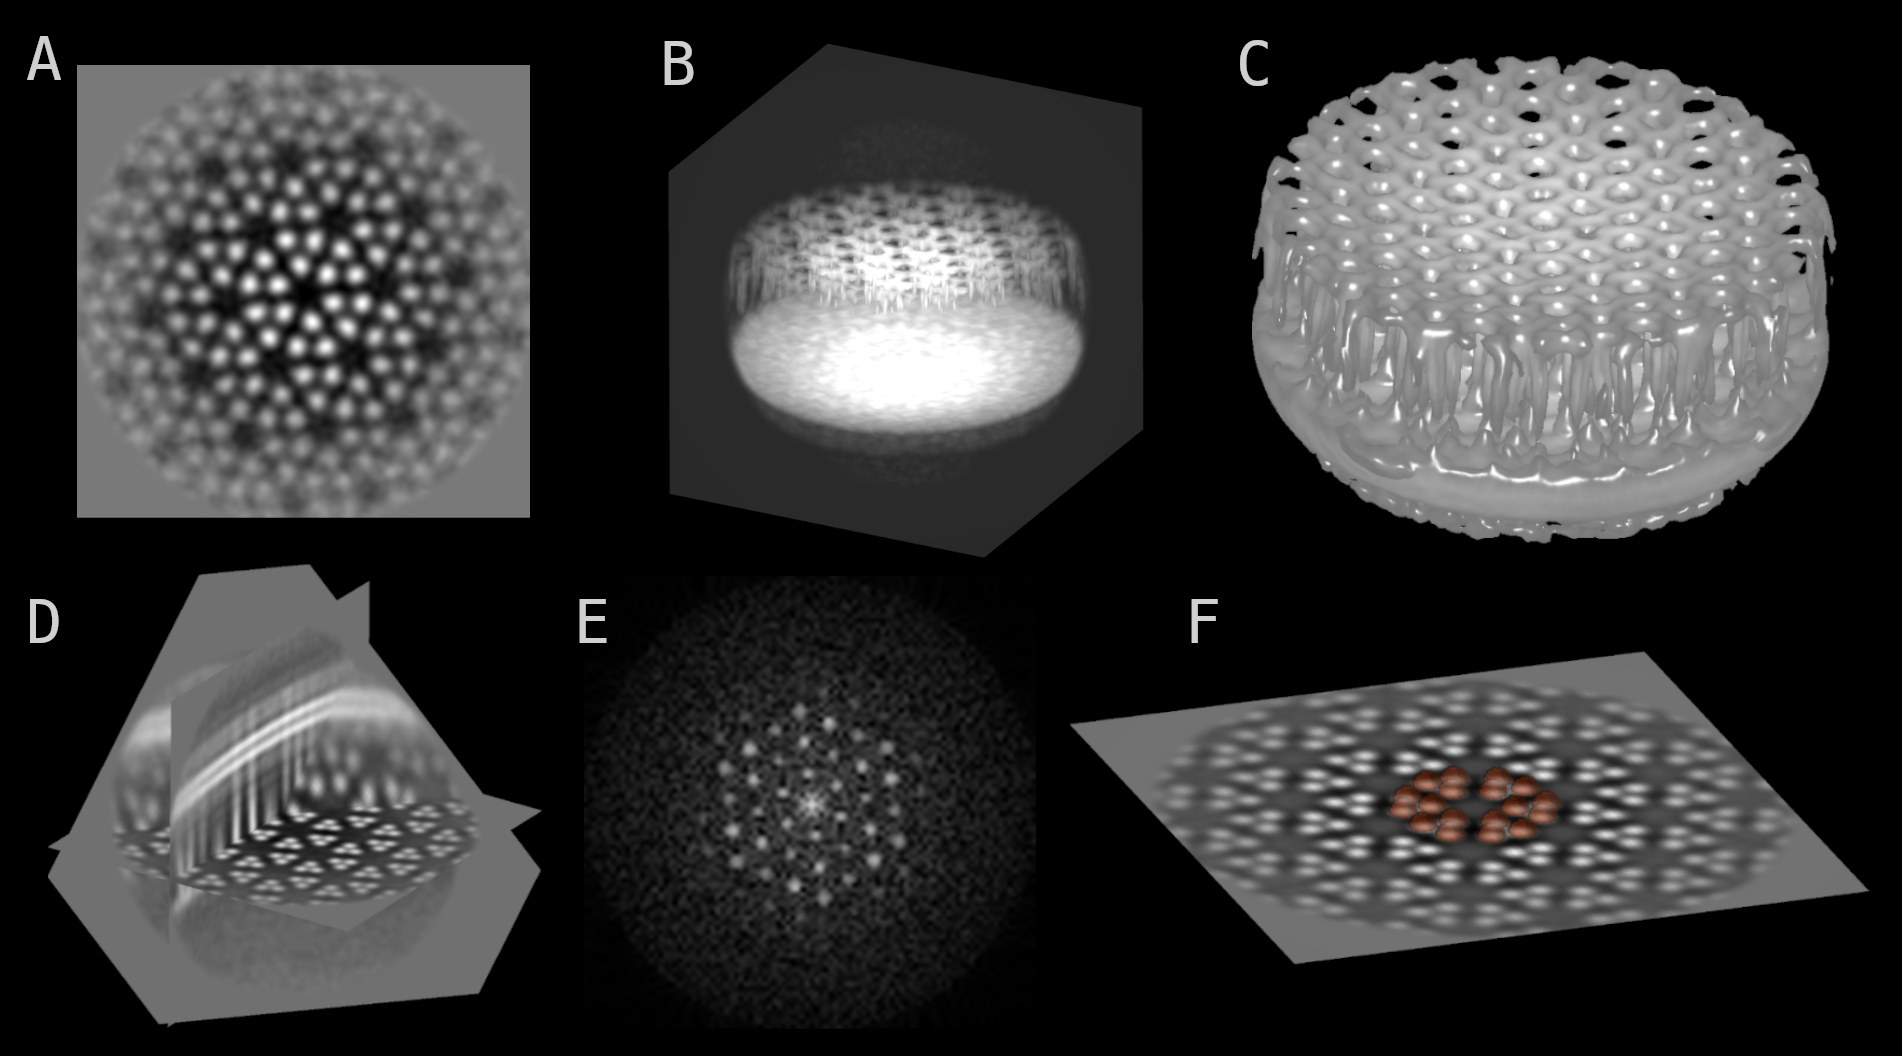
\includegraphics[width=\textwidth]{blik_paper/image_volume_showcase.png}
    \caption[Volume visualisations]{\textbf{Volume visualisations.} Showcase of the image visualisation capabilities of \texttt{napari} and \texttt{blik}. Chemoreceptor arrays of the \textit{E. coli} minicells~\cite{burtCompleteStructureChemosensory2020} are used for illustrative purposes throughout the figures. \textbf{A.} 2D slice through a 3D volume. \textbf{B.} Maximum intensity projection of the 3D volume. \textbf{C.} Isosurface. \textbf{D.} Arbitrary 3D plane slicing in 3D view. \textbf{E.} 2D slice through the 3D power spectrum of the volume. \textbf{F.} Segmentation (in semi-transparent brown) of 3D objects.}
    \label{images-showcase}
\end{figure}

\texttt{blik} also provides some widgets with extra functionality to complement image visualisation:

\begin{itemize} 
    \item A basic GPU-accelerated filtering tool (gaussian blur) for 2D images and 2D slices that is computed on the fly and whose parameters can be regulated with sliders. Simple gaussian filters are frequently used in image visualisation, especially with noisy cryo-EM data. While generating a filtered image is a relatively fast procedure, it is rarely fast enough to be computed on the fly on a CPU. GPU-accelerated filtering allows switching on and off on the fly, as well as changing kernel size and sigma, without having to generate a new image. While \texttt{blik} exposes only gaussian filtering, the underlying logic was implemented in the \texttt{vispy} OpenGL shader allowing for arbitrary convolutional kernels. Firstly, the image texture is sampled in a NxM grid (for a kernel of shape NxM) centered around the texture coordinates. A weighted average is then computed based on the kernel weights and the resulting value is forwarded to the rest of the shader. 
    \item A \texttt{power\ spectrum} widget, which quickly computes the power spectra of single images, stacks or volumes (\autoref{images-showcase}E). Power spectra are a fundamental tool for data inspection and validation in cryo-EM, from estimating resolution, to generating hypotheses about symmetry, to finding caveats in the data collection procedure. Like any other computation made by \texttt{blik} or \texttt{napari}, the power spectrum is then available as a normal \texttt{numpy} array for further use from within Python or to export to the available formats.
\end{itemize}

Additionally, masks and pixel-based segmentations (often called just ``segmentations'', or ``labels'' in \texttt{napari} jargon) are easily displayed (and modified with all the tools provided by \texttt{napari}, such as free-hand painting, even in 3D) by using the \texttt{napari} \texttt{Labels} layer, which is designed specifically to work with segmentation data (binary or integer arrays) (\autoref{images-showcase}F). Label processing is a particularly thriving area of the \texttt{napari} ecosystem, albeit mostly in the field of fluorescence and optical microscopy. This is a great opportunity for knowledge sharing and code reuse between fields that otherwise are typically relegated to separate software pipelines.

\subsubsection{Particles}\label{particles}

Particle data (coordinates, orientations, and any additional features and metadata) can be loaded from common formats (\texttt{.star}, \texttt{.tbl}). Coordinates are visualised as spheres, and orientations as basis vectors centred on the spheres (\autoref{particles-showcase}). Both components can be disabled or tweaked (such as color-coded or resized, labeled, etc.) for better visualisation. As with images, particles can be easily viewed in 3D.

\begin{figure}[!ht]
    \centering
    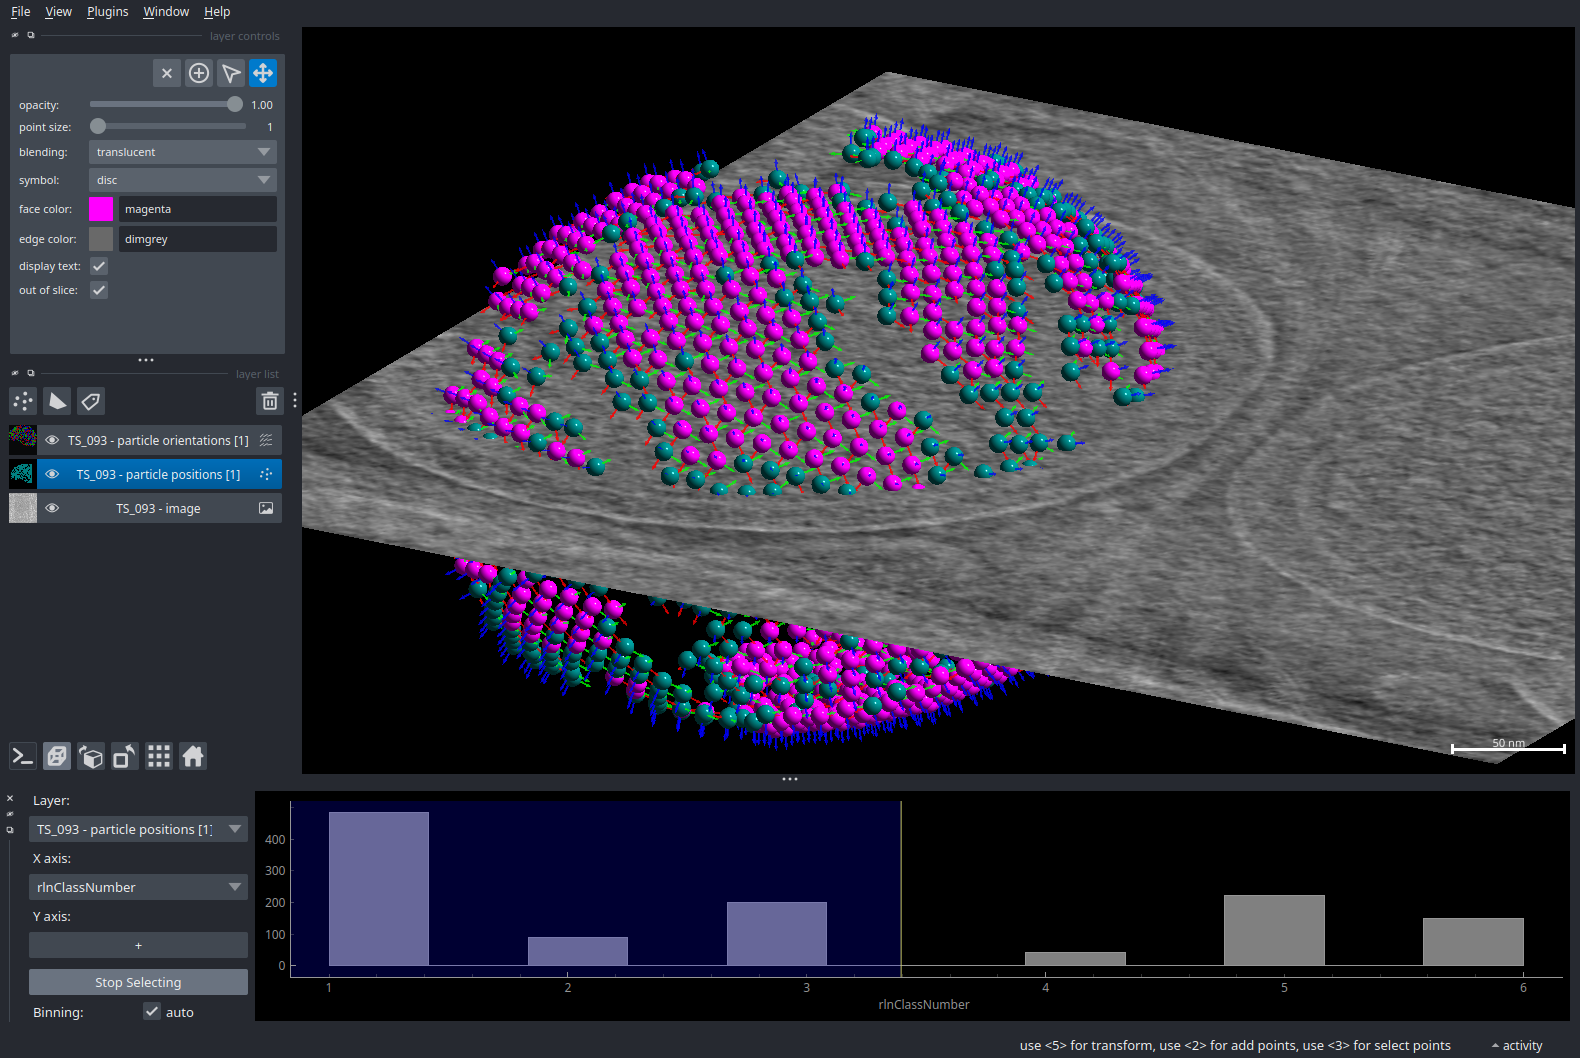
\includegraphics[width=\textwidth]{blik_paper/particle_plot.png}
    \caption[3D particle visualisation and feature plotting]{\textbf{3D particle visualisation and feature plotting.} Particles are from a \texttt{Relion} 3D classification of chemoreceptor arrays of the \textit{E. coli} minicells~\cite{burtCompleteStructureChemosensory2020}. Orientations are displayed with the three basis vectors in red/blue/green. The properties-plotter widget (bottom) shows a plot of a \texttt{Relion} data column -- in this case, the \texttt{rlnClassNumber} -- as a histogram. By selecting an area of this plot, the corresponding subset of particles is selected. This can be then used for further processing; in this case, selected particles are coloured differently (in magenta), showing that the selected classes contain mostly particles from the core of the chemoreceptor array lattice.}
    \label{particles-showcase}
\end{figure}

Since particles are actually simple \texttt{napari} \texttt{Points} layers, everything in the \texttt{napari} ecosystem that works with points will work with particles, such as manual or automated selection based on features, editing and coloring, classification, etc. Once again, the wealth of cross-field contributions towards the \texttt{napari} ecosystem is a valuable asset for processing data.

For example, points (and thus particles) may hold extra metadata in their \texttt{features} dataframe, such as classification results or quantitative values such as a confidence score. All such features can be used to encode visualisation parameters like color, rendered symbol (sphere, square, cross, etc.) and size, facilitating data inspection and selection of suitable candidates for further processing.

To fully take advantage of this, shipped as part of \texttt{blik} - but developed as a standalone field-agnostic \texttt{napari} plugin - is the \texttt{napari-properties-plotter} plugin, which allows interactive plotting of per-point features (\autoref{particles-showcase}, bottom widget), such as \texttt{Relion}'s figure of merit, classification results, resolution estimates, etc. Distribution histograms or scatter plots with any combination of features as axes can be automatically generated by simply selecting the desired features. Moreover, by picking subsections of such plots, particles can then be selectively rendered, modified, saved and otherwise processed.

\subsection{Input/Output}\label{input-output}

The reading, writing and conversion logic used by \texttt{blik} was developed as a standalone library, \href{https://github.com/teamtomo/cryohub/}{\texttt{cryohub}}. This library has a modular design to allow reuse in other applications and simplify the contribution of new formats. Currently, it supports the following formats for images and segmentations:

\begin{itemize}[noitemsep]
    \item \texttt{.mrc} (and the \texttt{.mrcs}, \texttt{.st}, \texttt{.map}, \texttt{.rec} variants) 
    \item \texttt{.tif(f)} 
    \item \texttt{Dynamo} \texttt{.em} 
    \item \texttt{EMAN2} \texttt{.hdf}
\end{itemize}  

\noindent and the following formats for particles:

\begin{itemize}[noitemsep]
    \item \texttt{Relion} \texttt{.star} (Relion $\geq$ 3.0)
    \item \texttt{Dynamo} \texttt{.tbl} 
    \item \texttt{CrYOLO} \texttt{.cbox} and \texttt{.box}
    \item \texttt{EMAN2} \texttt{.json}
\end{itemize}

Where possible, \texttt{blik} makes use of lazy loading via \texttt{dask}~\cite{daskdevelopmentteamDaskLibraryDynamic2016}, which allows working with data that is larger-than-memory and loading full datasets at once for ease of browsing.

\subsection{Image segmentation}\label{image-segmentation}

A few annotation and analysis tools were implemented as part of \texttt{blik} or standalone \texttt{napari} plugins.

The \texttt{napari} community has already developed numerous plugins for segmentation and annotation of 2D and 3D imaging data, spanning from manual annotation and traditional image-processing-based segmentation to AI tools. \texttt{blik}'s current contributions to this ecosystem are in some cases general-purpose -- such as utilities for manual annotation of volumetric segmentations -- and in other cases focused on cryo-ET-specific issues that are not easily solved by existing methods -- such as rigorous geometry-based particle picking on filaments and surfaces.

Pixel-based image segmentation is already natively supported in \texttt{napari} through the \texttt{Labels} layer, with mature tools for editing, data exploration and annotation. One previously missing feature is the ability to easily interpolate labels from sparsely annotated 2D slices of a 3D volume into full 3D volumetric labels. \texttt{blik} brings a standalone plugin for this purpose called \texttt{napari-label-interpolator} (\autoref{interpolator-showcase}), which works with any \texttt{Image} layer and interpolates n-dimensionally (e.g: it can interpolate 3D labels over a time series).

\begin{figure}[!ht]
    \centering
    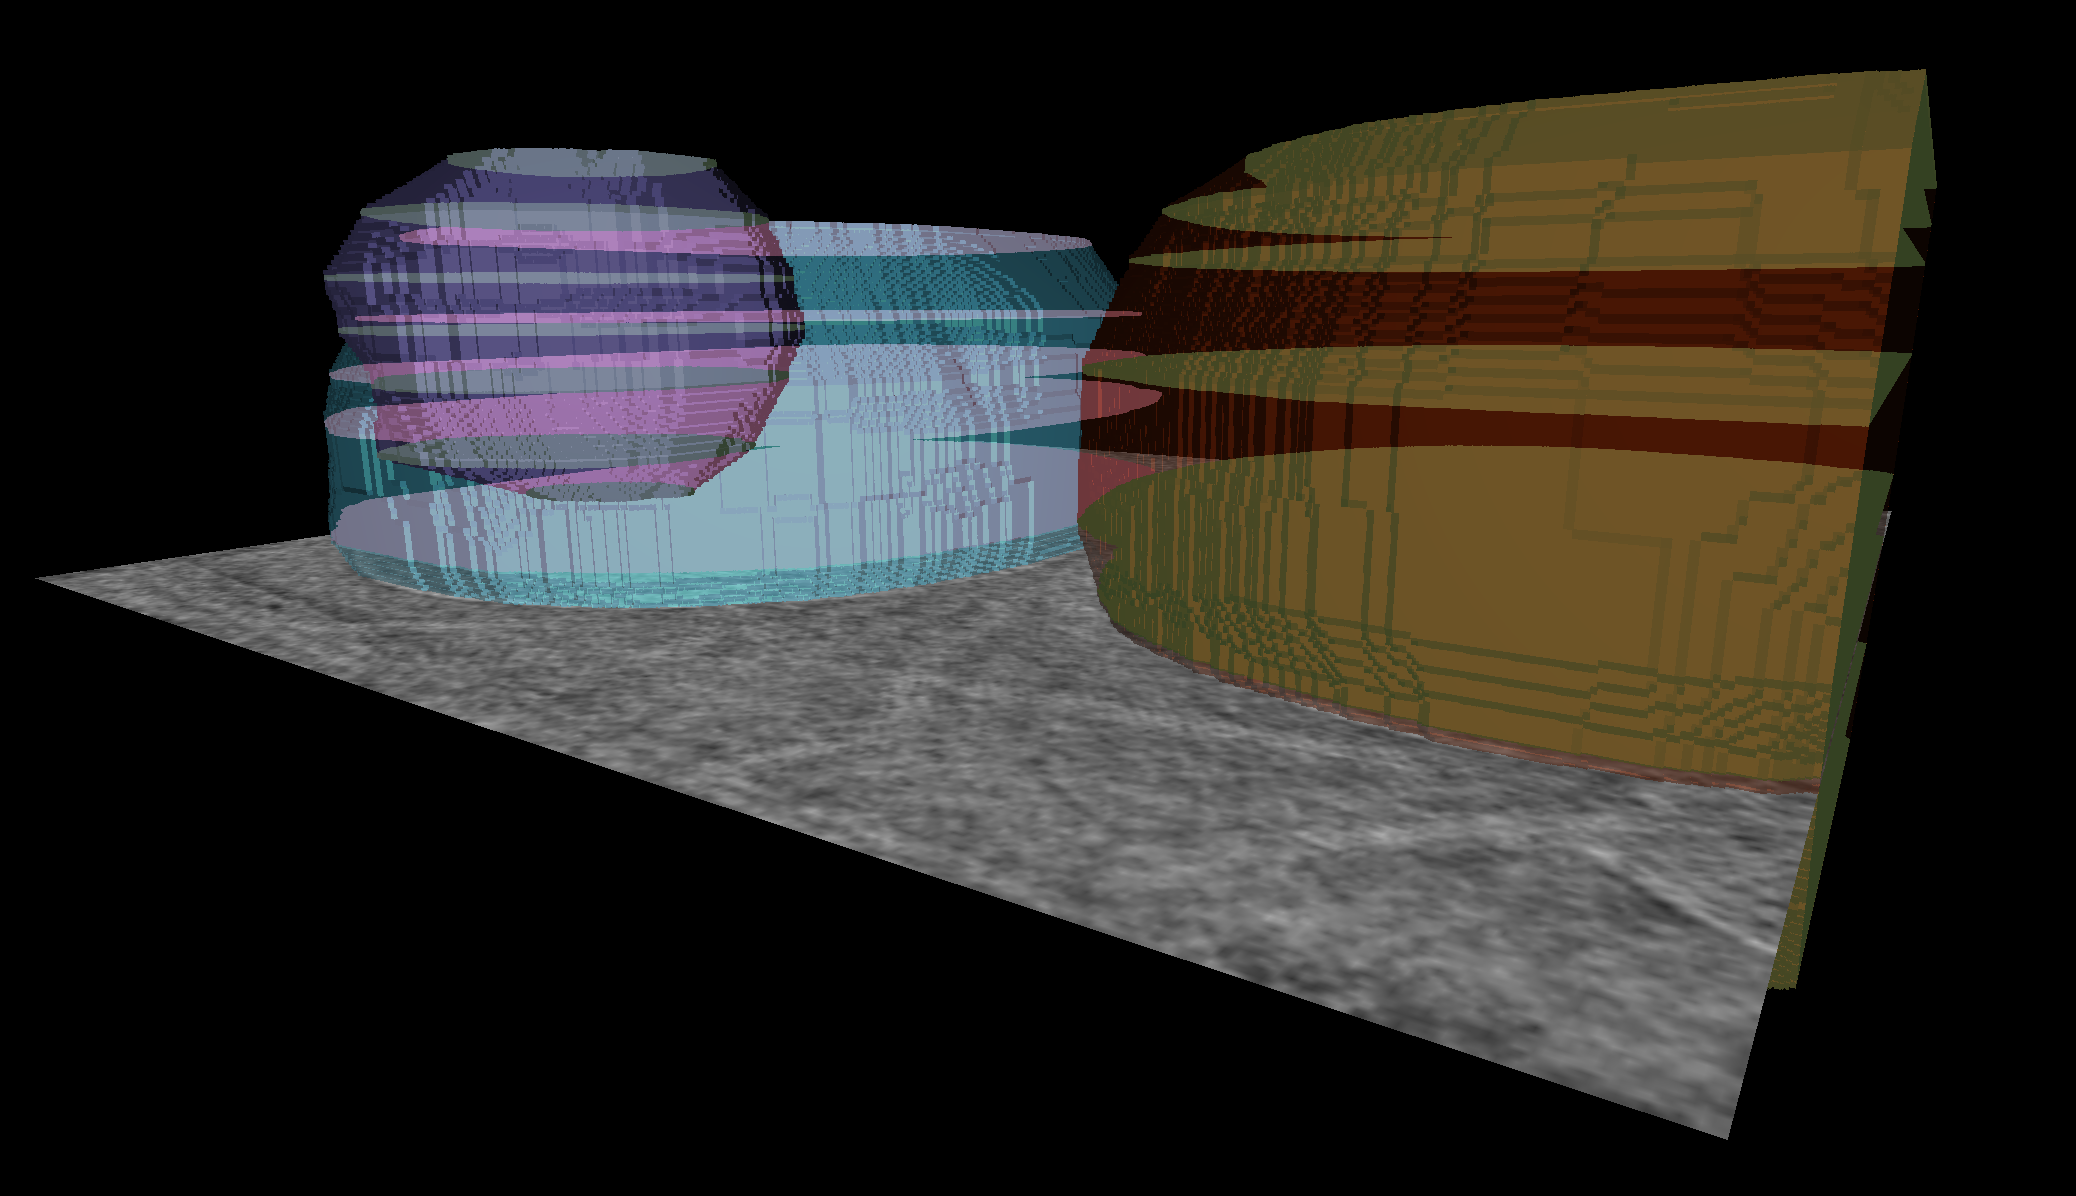
\includegraphics[width=\textwidth]{blik_paper/segmentation_showcase.png}
    \caption[Interpolated segmentations]{\textbf{Interpolated segmentations.} A tomogram is manually annotated on a few 2D slices using the \texttt{napari} labels painting functionality. These sparsely annotated 2D slices are then interpolated with the label interpolator widget to generate a volumetric segmentation of multiple objects.}
    \label{interpolator-showcase}
\end{figure}

The plugin works by interpolating Signed Distance Fields (SDF) across multiple n-dimensional slices. For each annotated slice along the interpolation dimension and for each label, the (n-1)-dimensional SDF is computed. SDF slices are then linearly interpolated with a simple weighted average, with weights proportional to the distance from the neighboring annotated slices. Where the weighted average is greater than zero, the voxel is considered to be part of the interpolated label.

This system plays very well with volumetric annotation, but has limits with thin labels such as filaments or surfaces. We plan to add different types of interpolation in order to widen the scope of application and usability of this tool.

\subsection{Filament and surface generation}\label{filament-and-surface-generation}

A different kind of image segmentation uses mathematical representations such as filaments, surfaces and fields to describe morphological features. In this context, \texttt{blik} contributions were made to a general-purpose library at \href{https://github.com/morphometrics/morphosamplers}{\texttt{morphometrics/morphosamplers}}, which aims to provide generalised morphological descriptions and sampling for scientific imaging. Specifically, we developed a helical filament model based on parametric splines, as well as a parametrised spline-grid surface model which allows to rigorously annotate surface-like objects such as membranes from simple point annotations.

The \texttt{morphosamplers} code was implemented with two main goals: keeping the manual annotation procedure simple and robust, and generating ordered, regularly spaced poses that can be used both for particle picking for subtomogram averaging and to allow volume resampling (see \nameref{resampling}). Picking particles as a regularly spaced lattice can significantly improve the results of subtomogram averaging when it reflects the underlying geometry of the sample~\cite{castano-diezDynamoCatalogueGeometrical2017,burtFlexibleFrameworkMultiparticle2021}. Model picking tools in \texttt{Dynamo}~\cite{castano-diezDynamoFlexibleUserfriendly2012} had a strong influence on the purpose and functionality of \texttt{blik}; unlike the \texttt{Dynamo} mesh-based approach, the spline-based implementation aims to optimise regular Euclidean spacing and consistency in initial particle positioning and orientations.

\subsubsection{Filaments}
Filament picking (\autoref{filament-pick}) uses a relatively simple single-spline approach:

\begin{itemize}[noitemsep]
    \item Points are picked manually in 3D space along the filament.
    \item A spline representation is generated, parametrised so that samples are equidistant in Euclidean space.
    \item Given a specific rise and twist, particles are generated along the spline in a helical pattern.
    \item If a radius is given, the particles are shifted away from the spline by that amount.
    \item If a symmetry group is given, symmetric copies are created around the filament axis.
\end{itemize}

\begin{figure}[!ht]
    \centering
    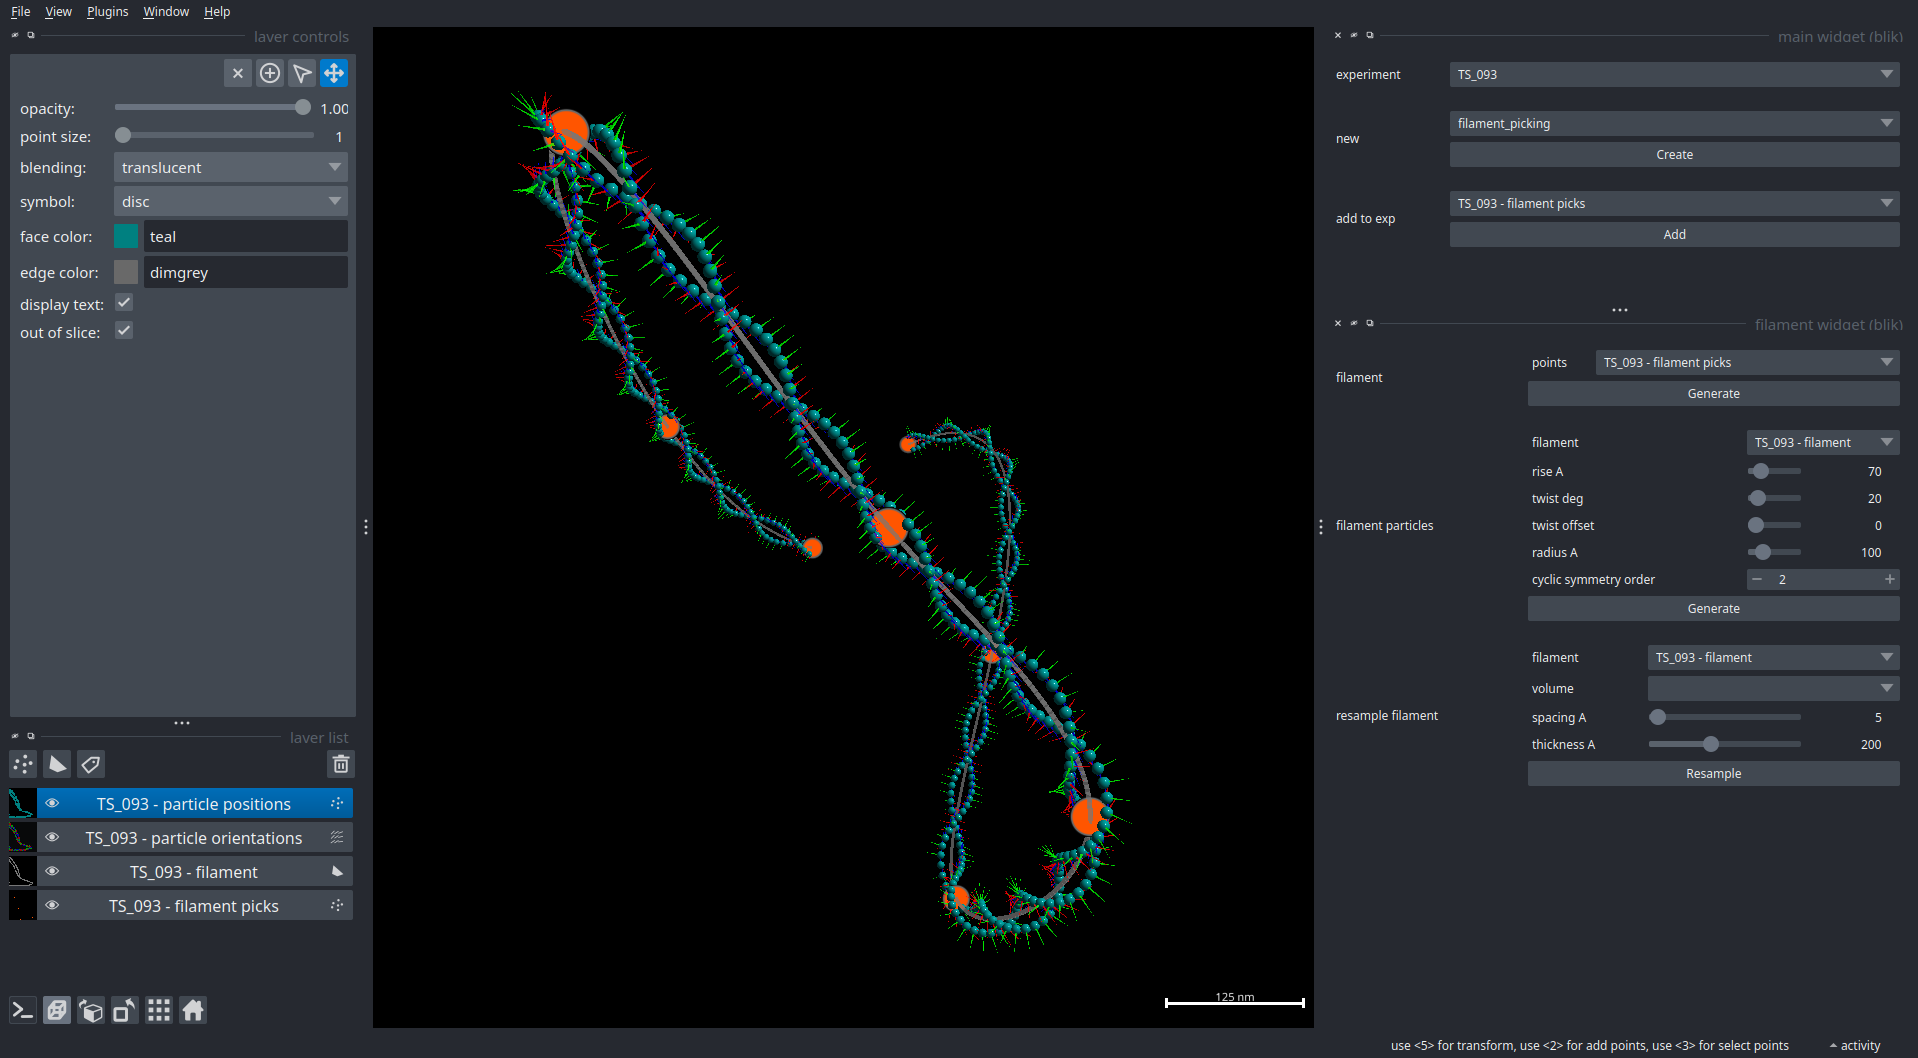
\includegraphics[width=\textwidth]{blik_paper/filament_pick.png}
    \caption[Filament-based particle picking]{\textbf{Filament-based particle picking.} Particle picks along a helical filament generated by \texttt{blik}. Starting from simple points picked manually along the desired path (orange points) and using the filament widget (on the right), a spline representation is computed (grey) and used to generate particle poses (cyan spheres with basis vectors) according to the given helical parameters defined in the widget.}
    \label{filament-pick}
\end{figure}

\subsubsection{Surfaces}
The surface generation uses the same underlying parametric spline logic as filaments, but creates a grid of splines to capture the surface shape (\autoref{surface-pick}). The procedure can be broken down into the following steps:

\begin{itemize}[noitemsep] 
    \item A few points are picked along the desired surface, repeating at different Z-slices.
    \item For each Z-slice annotated as such, a parametric spline (with desired interpolation order and smoothing) is computed.
    \item Points are distributed uniformly on these splines, ensuring equidistance in Euclidean (and not parametric) space.
    \item The resulting strips of points are then aligned by minimising index-wise distances, and padded to enforce a rectangular grid.
    \item New splines are then computed, by using the generated points as control points. This results in parallel splines, perpendicular to the first set and equidistant from each other.
    \item New points are then generated on this second group of splines, similarly to the first round, equidistant in Euclidean space. This results in a full rectangular grid of equidistant points.
    \item A third group of splines is generated in the same orientation as the first group.
    \item The second and third group of splines are used to compute the derivatives; this gives - for each point on the surface - two vectors tangent to the surface and perpendicular to each other. With these, normal vectors are calculated, giving the full orientation of each particle on the surface.
\end{itemize}

Parameters such as interpolation order, inter-particle distance, and smoothing can be controlled, allowing fine-tuning of the generated surface.

While this approach is advantageous for relatively regular surfaces, for which the generated grid of splines provides uniformly spaced and oriented points on the surface, its main downside is that complex surfaces will inevitably deform the grid. This method struggles especially with strongly irregular surfaces, such as membranes with numerous invaginations located at different Z-slices.

\begin{figure}[!ht]
    \centering
    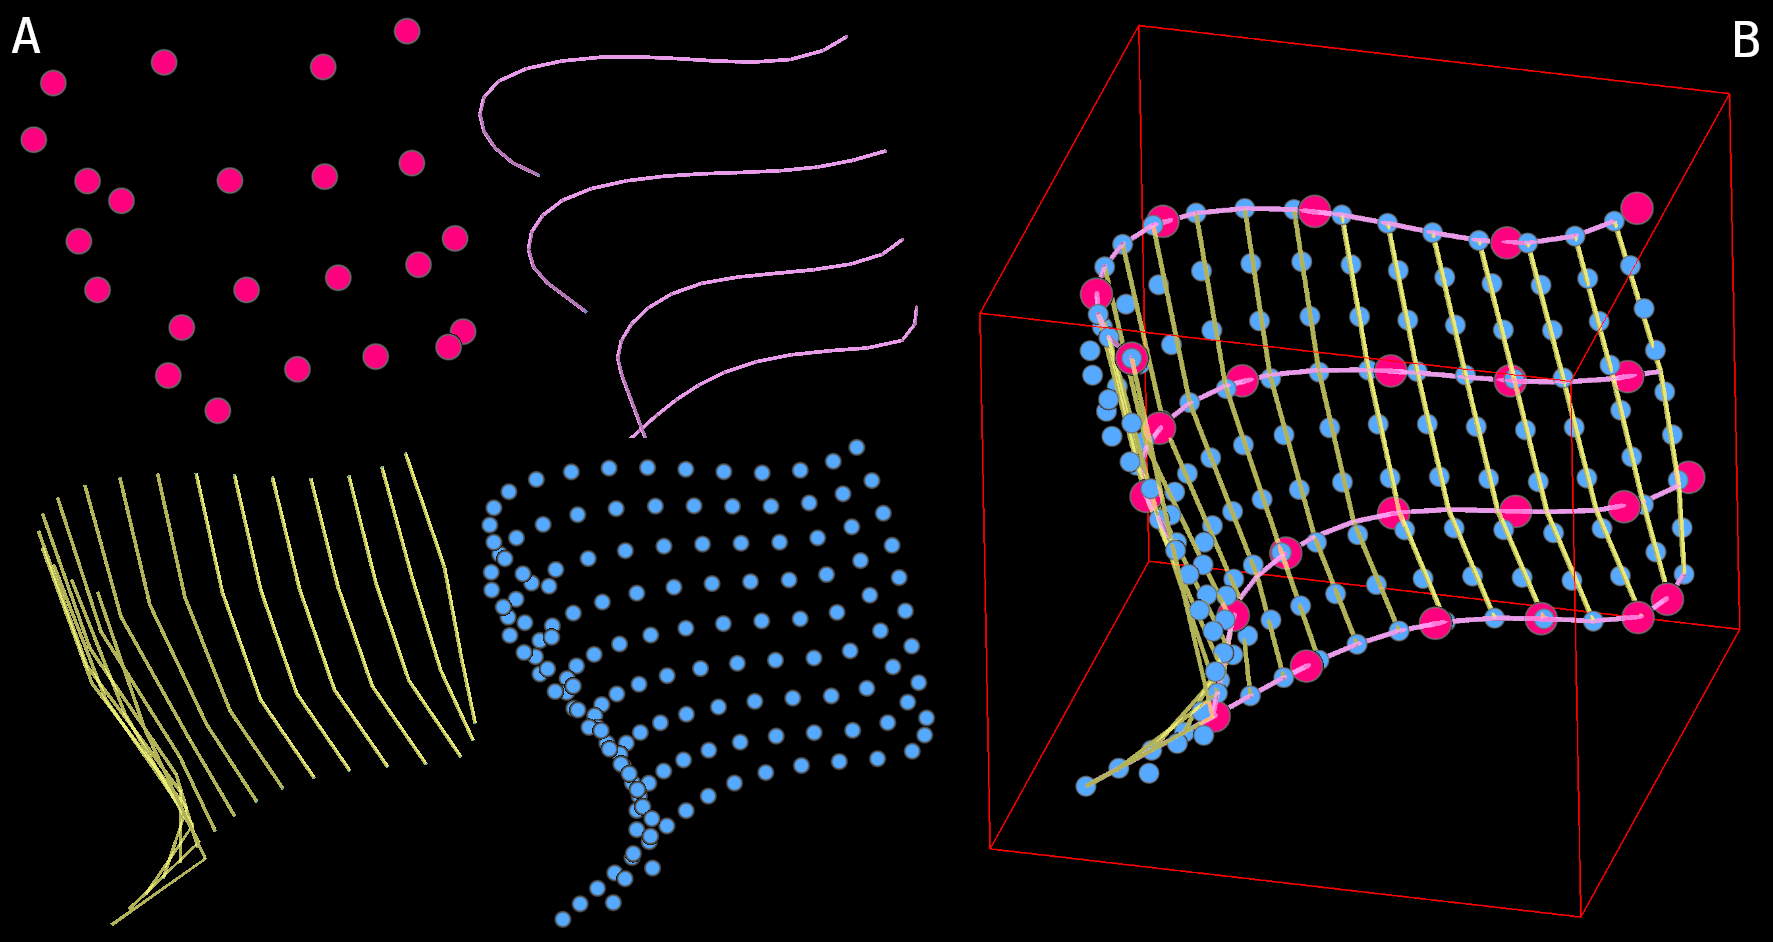
\includegraphics[width=\textwidth]{blik_paper/spline_grid_showcase.png}
    \caption[Surface generation procedure]{\textbf{Surface generation procedure.} \textbf{A.} Step-by-step procedure used by \texttt{blik} to generate surfaces. An initial set of points (magenta) is picked on a few Z-slices following the desired surface. A first set of splines (purple) is generated within each Z-slice, and then used to generate equidistant samples which become the nodes of the next set of splines, perpendicular to the first (yellow). The second set of splines is then resampled with the same spacing, thus generating a final set of grid-like, evenly spaced samples. \textbf{B.} All the steps combined.}
    \label{surface-pick}
\end{figure}

\subsubsection{Resampling}\label{resampling}
The grid-like, regularly spaced nature of these models can be additionally used to create visualisation aids (meshes and filaments) and to resample the annotated volume along the annotated object. Such volume resampling can be useful for quantitative and spatially consistent volume analysis of otherwise complex 3D objects; density profiles of a complex 3D surface can thus be generated while retaining spatial information. In practice, this can also be used to aid visualisation, by ``straightening'' an otherwise curved surface.

\begin{figure}[!ht]
    \centering
    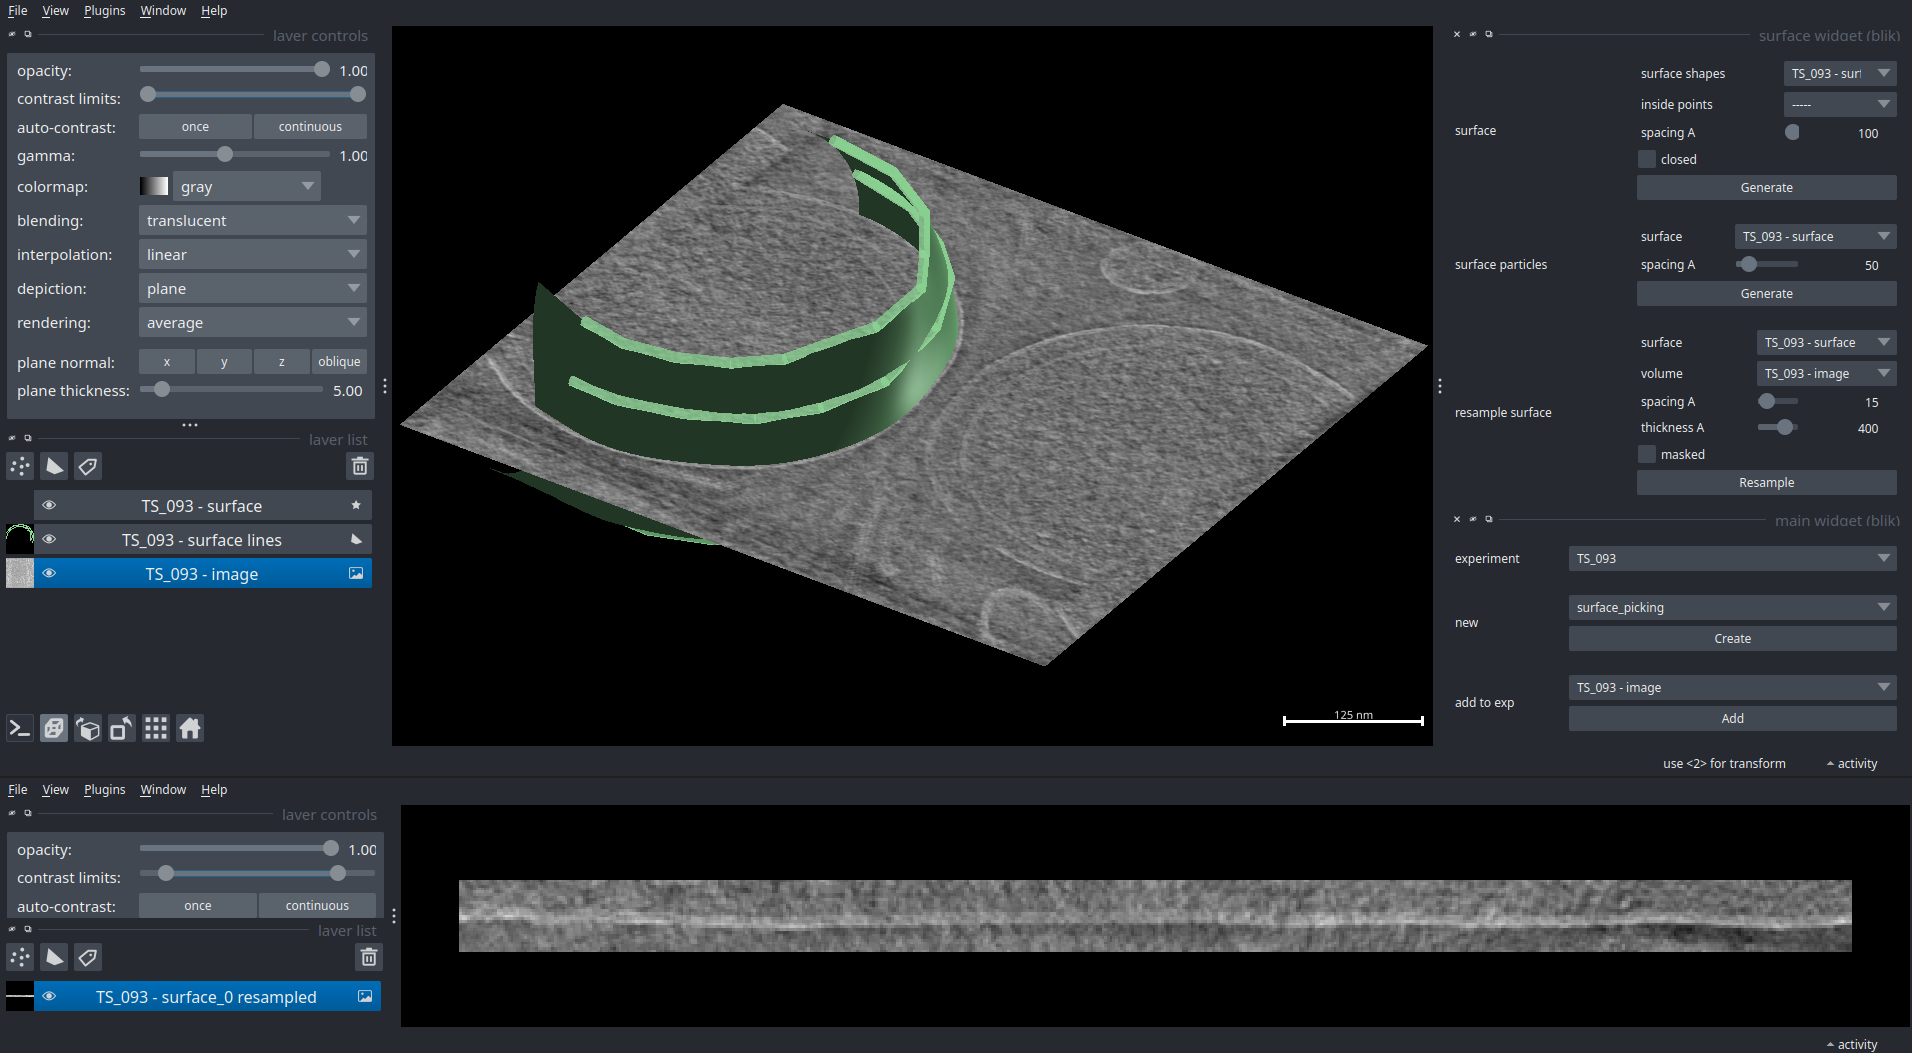
\includegraphics[width=\textwidth]{blik_paper/surface_resample.png}
    \caption[Surface-based volume resampling]{\textbf{Surface-based volume resampling.} \textbf{Top}: a surface is generated using the surface widget, following the shape of a minicell membrane. The tomogram volume is then resampled based on the picked surface and a few parameters set in the widget, such as sample thickness and pixel spacing. \textbf{Bottom}: the result is a 3D volume containing a ``straightened'' version of the picked surface, displayed here averaged along Z into a 2D image.}
    \label{surface-resample}
\end{figure}

\subsection{Particle picking}\label{particle-picking}

\texttt{blik} provides a few tools for picking particles for subtomogram averaging. All such particles can then be saved in the formats implemented by \texttt{cryohub} for further processing.

\begin{figure}[!ht]
    \centering
    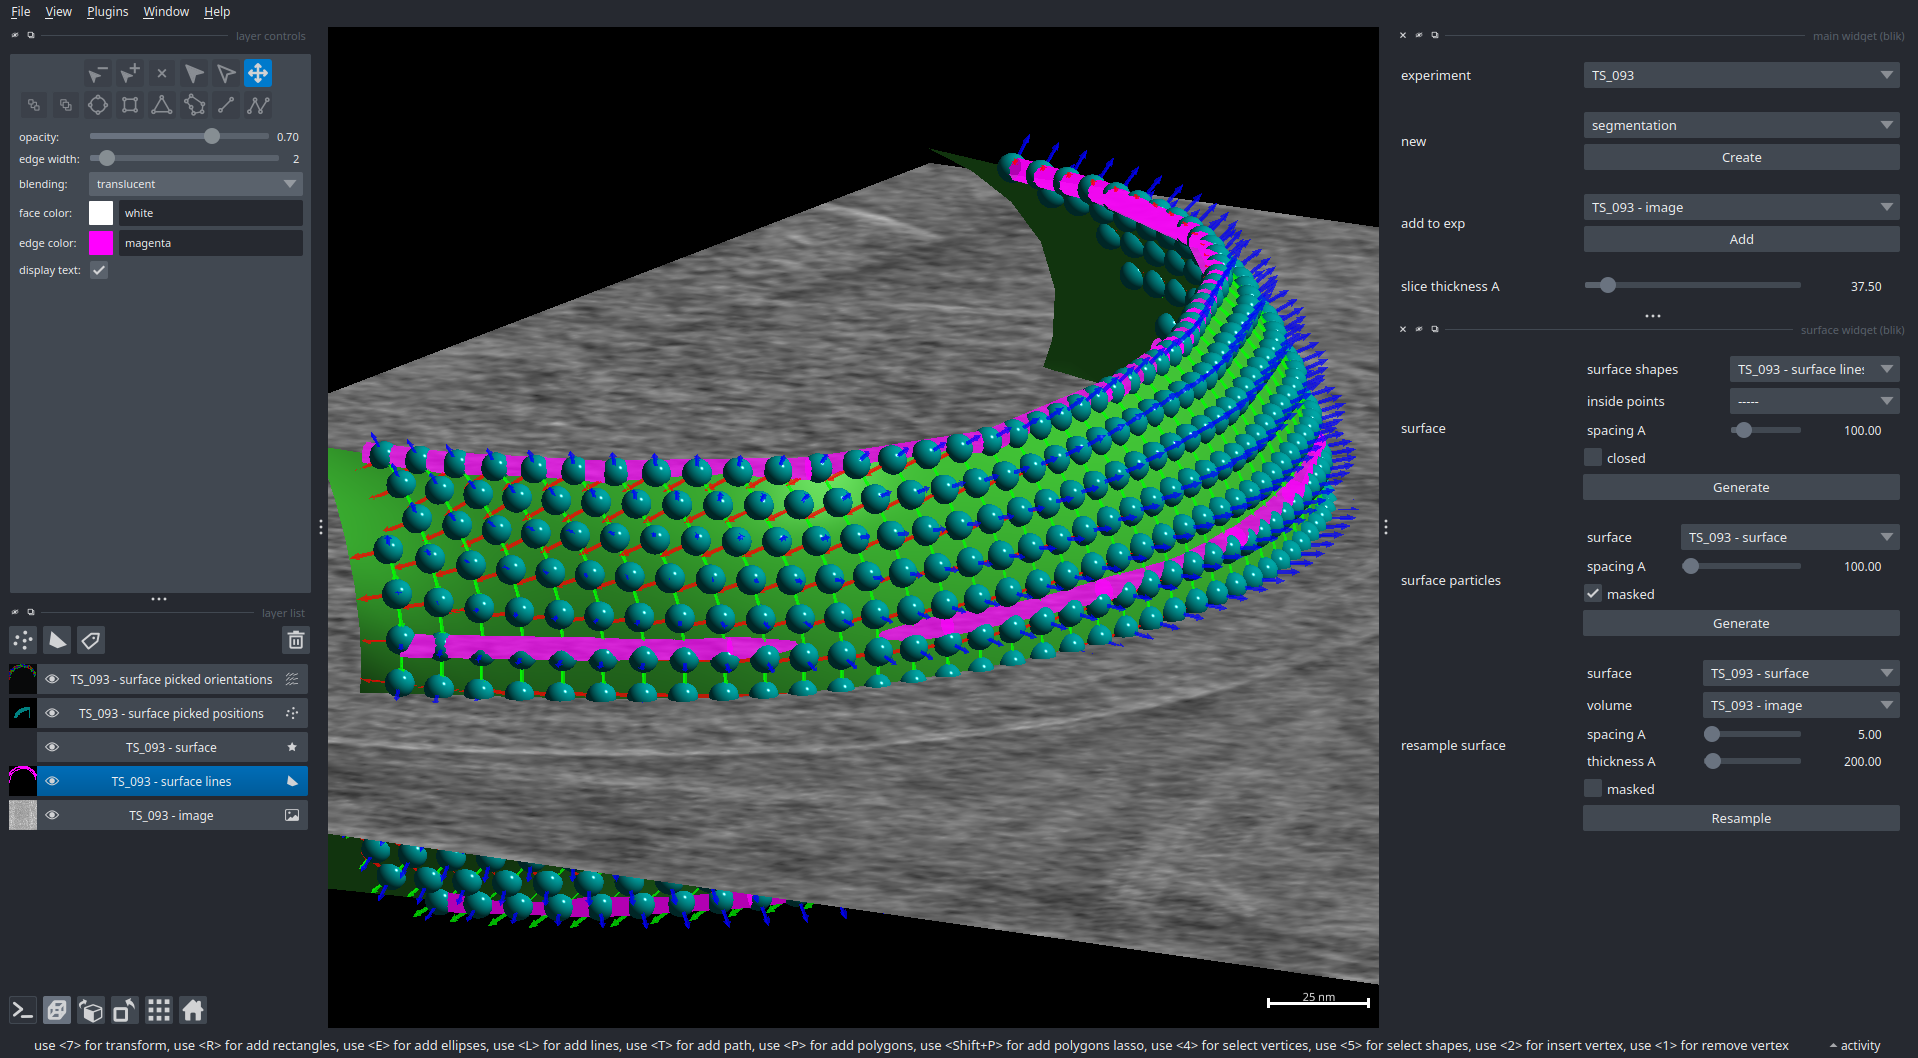
\includegraphics[width=\textwidth]{blik_paper/surface_particles_mesh.png}
    \caption[Surface mesh and particle picks]{\textbf{Surface mesh and particle picks.} A surface is generated using the surface widget, starting from the manually picked lines (magenta) which follow the shape of a chemosensory array. The generated surface is displayed as a mesh (green). Particles for subtomogram averaging (cyan spheres and red/green/blue basis vectors) are then generated based on a few parameters set in the surface widget (on the right).}
    \label{picking-showcase}
\end{figure}

The most basic picking tool is a manual picker; simply clicking points on an image or volume slice will generate a particle in that position. Manually modifying the orientation is not yet implemented, but is planned for a future release.

For more complex picking, the aforementioned filament and surface models can also be used to generate particles (\autoref{picking-showcase}). These will be regularly distributed on the surface with a provided inter-particle spacing, and oriented with their Z basis vector along the filament axis, or the normal of the surface. This is useful for initialising particle picks for objects following an underlying geometry, such as helical filaments and membrane proteins, and is particularly suited for dense lattices.

\subsection{Scipion Integration}\label{scipion-integration}

To ease the integration of \texttt{blik} into existing workflows, we also release a \href{https://github.com/scipion-em/scipion-em-blik}{\texttt{blik} Scipion plugin}. This plugin exposes all of \texttt{blik}'s main functionalities (visualisation, segmentation and particle picking) as Scipion protocols which can be used in combination with all the existing tomography protocols provided by Scipion and other plugins.

\section{Discussion}
With \texttt{blik}, we add to the cryo-ET software ecosystem an integratable and interactive data viewer, radicated in the Python ecosystem, and a reusable and extensible set of libraries and tools for annotation and picking. There are several existing tools with similar goals and functionality to \texttt{blik}; in this section, we discuss the most widely-used options known to us, examine their compatibility with \texttt{blik} and compare their features with our tool. This should provide a starting point for the reader to choose the appropriate tool for their project.

\vspace{\baselineskip}

\texttt{blik} was tested primarily to work within the \texttt{Relion}\&Warp pipeline~\cite{scheresRELIONImplementationBayesian2012,tegunovMultiparticleCryoEMRefinement2021,burtFlexibleFrameworkMultiparticle2021}, but was designed to be workflow-independent and thanks to \texttt{cryohub} easily extensible with new data formats. Following this workflow, other than the ubiquitous \texttt{.mrc} image format and \texttt{Relion}'s \texttt{.star} particle format, one of the first compatibilities to be developed was with image and particle data from the \texttt{MATLAB} software suite \texttt{Dynamo}~\cite{castano-diezDynamoFlexibleUserfriendly2012} and its processing pipeline. \texttt{Dynamo} provides its own visualisation and picking tools, which were also the main inspiration for the geometry-based filament and surface particle generation in \texttt{blik}. While particle picking in \texttt{blik} has currently a smaller scope compared to \texttt{Dynamo}, its implementation in Python is intended to be more easily maintained and extended in the future by users, while leveraging the full-featured \texttt{napari} visualisation.

\texttt{IMOD}~\cite{kremerComputerVisualizationThreeDimensional1996} is arguably the giant in the field, with a long history of development and a wealth of features for image processing and annotation. Given its extensive capabilities and the constant development, it is usually the first choice when it comes to cryo-EM/ET processing, visualisation, and annotation. Many of these features are very useful, and we plan to add support for them in \texttt{blik} or \texttt{napari} in the future. Integration between \texttt{blik} and \texttt{IMOD} is seamless for most common operations, such as working with data processed through \texttt{IMOD}'s tomography pipeline \texttt{etomo}. \texttt{IMOD}'s 3d viewer \texttt{3dmod} is full-featured and fast, and has several modes for 2D projection and slicing. It has however a more limited 3D renderer compared to \texttt{napari} (no volumetric projections, slicing planes in 3D view, or native particle pick viewer), which limits its applicability for the inherently 3D work of tomography. Being written in C, it is also non-trivial to extend for users with limited programming knowledge.

ThermoFisher's Amira~\cite{thermofisherAmiraSoftwareLife} is also a popular choice for image visualisation and annotation. It is particularly appreciated for its easy-to-use labeling tools to improve manual annotation and tracing, such as label interpolation, and image-guided picking. Amira's label interpolation was the main inspiration behind \texttt{napari-label-interpolator}, and image-guided picking is in the future plans for \texttt{blik} development. Being an image-focused tool, Amira is more limited when it comes to particle coordinate generation although it has some model-based filament picking that can be repurposed for particle generation with the help of user scripts. However, Amira's closed-source proprietary nature is a big downside for open science practices, making it hard or impossible to extend, contribute to, and freely share within the scientific community.

\texttt{EMAN2}~\cite{galaz-montoyaSingleParticleTomography2015} is a full software suite with an entire tomography pipeline from raw data to reconstruction. I/O compatibility between \texttt{EMAN2} and \texttt{blik} is partially implemented, allowing to read particles and tomograms. \texttt{EMAN2} has some tools for visualisation and picking, and is especially powerful for automated picking and segmentation thanks to machine learning tools. Its 3D visualisation is similar to \texttt{IMOD} in features.

Tomviz~\cite{schwartzRealtime3DAnalysis2022} is an open-source application focusing on tomogram reconstruction and visualisation, providing also a few segmentation and analysis tools.

\vspace{\baselineskip}

When it comes specifically to particle picking and visualisation, a powerful tool recently developed is \texttt{ArtiaX}~\cite{ermelArtiaXElectronTomography2022}, a \texttt{ChimeraX}~\cite{pettersenUCSFChimeraXStructure2021} extension for cryo-ET. Thanks to \texttt{ChimeraX}'s beautiful ray-tracing renderer, \texttt{ArtiaX} is ideal to make figures for publications. Particle visualisation is also very convenient and allows even for visualising subtomogram averaging results (map isosurfaces) distributed on the tomograms thanks to a performant implementation with instanced rendering. \texttt{ChimeraX} also provides a Python API to control its visualisations, but doesn't offer the same level of two-way and direct access to the visualised data as \texttt{napari} with its \texttt{IPython} console. \texttt{ChimeraX}'s features and ecosystem are also more focused on protein structure visualisation and analysis, whereas \texttt{napari} is first and foremost an imaging tool.

Another tool that \texttt{blik} already integrates with is \texttt{CrYOLO}~\cite{wagnerSPHIREcrYOLOFastAccurate2019}, which provides powerful machine-learning picking and segmentation routines. \texttt{CrYOLO} itself has recently adopted \texttt{napari} as its visualisation front-end.

A similar tool to the surface resampling widget in \texttt{blik} exists in \texttt{Membranorama}~\cite{tegunovDtegunovMembranorama2024,wietrzynskiChartingNativeArchitecture2020}, which allows for visualising surfaces in a tomogram with the surrounding volume projected perpendicularly onto the surface, as well as extracting individual surface patches which can be "planarised" for easier inspection. This tool is very useful for interactive visualisation and exploration of the projected surface \texttt{in situ}. \texttt{blik}, on the other hand, does not allow \texttt{in situ} projection, but instead focuses on generating a square-grid resampling which -- differently from Membranorama -- can be exported as an ordinary volume or reused immediately for further processing with \texttt{blik} or other tools.

\vspace{\baselineskip}

Given the popularity and fast growth of Cryo-ET, the field offers many other tools and software suites with features and goals compatible with \texttt{blik}. Some of of them offer excellent opportunities of integration with the \texttt{napari} and \texttt{blik} ecosystem, such as \texttt{TomoSegMemTV}~\cite{martinez-sanchezRobustMembraneDetection2014} and \texttt{MemBrain}~\cite{lammMemBrainDeepLearningaided2022,lammMemBrainV2Endtoend2024}, which offer pixel-based and automated membrane segmentation (as opposed to the manual, surface-based annotation provided by blik) or \texttt{pycurv}~\cite{salferReliableEstimationMembrane2020} and \texttt{surface-morphometrics}~\cite{baradQuantifyingOrganellarUltrastructure2023}, which can compute meshes, measurements and statistics about pre-annotated membranes. With a collaborative and modular approach to software development, we strive for \texttt{blik} and \texttt{teamtomo} to become a starting point to enable such integrations in the future.

\section{Conclusion}

The work presented in this paper aims to reduce the friction of working with cryo-ET data, and to enable developers in the field to share, reuse and contribute as a community. The development of \texttt{blik} and its components is a stepping stone towards these goals.

Working within \texttt{napari} allows us to delegate (and share with other fields) many non-cryo-ET-specific components, while retaining interactivity and extensibility; \texttt{napari} is in rapid development, and direct contributions to the community-developed project are always welcome. Even where direct contributions are unfeasible, developers can take advantage of the plugin ecosystem (such as \texttt{blik} does) or simple scripting.

Now that \texttt{blik}'s core features are established, we aim to reach out to other developers and cryo-ET software users and encourage reusing, adopting or contributing to the work here presented.

Future planned features for \texttt{blik} include:

\begin{itemize}[noitemsep] 
    \item Exploit \texttt{napari}'s nD visualisation, for example to easily view the progression of a particle refinement.
    \item Conclude the work on \texttt{napari} multicanvas, allowing multiple views on the data (e.g: picking in orthoviews).
    \item Implement instanced rendering in \texttt{vispy} to allow rendering full particle maps in the tomogram at high performance (like \texttt{ArtiaX}).
    \item Offer more geometric models for picking (e.g: spheres, 3D lattices).
\end{itemize}

\section{Materials and methods}
Not all the code contributions from this work live in the same place. Tools and implementations were split into standalone libraries or contributed to core \texttt{napari} when possible, in the interest of sharing and avoiding code duplication. Contributions from work in this paper are summarised below, and readers are encouraged to take advantage of all these open-source components for their own work.

Refer to the individual repositories for the most up-to-date and in-depth documentation.

\subsection{cryotypes and cryohub}\label{cryotypes-and-cryohub}

The data structures and input/output (IO) functions used by \texttt{blik} are extracted into two usage-agnostic libraries: no assumptions from \texttt{blik} are carried over, which makes these libraries suitable for adoption by any Python software working with cryo-EM and cryo-ET data. Both libraries live in the github community project \href{https://github.com/teamtomo/}{\texttt{teamtomo}}.

\begin{itemize}[noitemsep] 
    \item \href{https://github.com/teamtomo/cryotypes/}{\texttt{cryotypes}}: defines simple and extensible data structures for cryo-EM data types and metadata, and provides simple validation and checking functions to ensure a given object conforms to the specification. 
    \item \href{https://github.com/teamtomo/cryohub/}{\texttt{cryohub}}: provides reading and writing functions for popular image formats and particle data, with both fine-grained controls and a higher level ``magic'' interface (\texttt{cryohub.open(\textless{}anything\textgreater{})}). Data is read to and from \texttt{cryotypes} data structures, easily allowing for conversion between formats and integration in any third-party Python tool.
\end{itemize}

\texttt{cryohub} provides granular I/O functions such as \texttt{read\_star} and \texttt{read\_mrc}, which will all return objects following the \texttt{cryotypes} specification.

\begin{minted}{python}
from cryohub.reading import read_star

poseset = read_star('/path/to/file.star')
\end{minted}

A higher-level function called \texttt{read} adds some magic to the IO procedure, guessing file formats and returning a list of \texttt{cryotypes}.

\begin{minted}{python}
from cryohub import read

data = read(
    '/path/to/file.star',
    '/path/to/directory/',
    lazy=False,
    name_regex=r'tomo_\d+'
)
\end{minted}

See the help for each function for more info.

Similarly to the \texttt{read\_*} functions, \texttt{cryohub} provides a series of \texttt{write\_*} functions, and a magic higher-level \texttt{write} function.

\begin{minted}{python}
from cryohub import write

write([poseset1, poseset2], 'particles.tbl')
\end{minted}

\subsection{morphosamplers}\label{morphosamplers}

Surface and filament picking and particle generation code are not specific to cryo-ET. They were developed as part of a field-agnostic library called \href{https://github.com/morphometrics/morphosamplers}{\texttt{morphosamplers}}, which collects several tools for sampling image data with morphological objects. As part of this work, models for spline filaments and spline-based surfaces were developed, with their relative tools for particle generation and image resampling.

\subsection{napari plugins}\label{napari-plugins}

Some of the \texttt{napari}-specific functionalities developed for \texttt{blik} were also not cryo-EM-specific, and could instead be useful for many other applications in the \texttt{napari} ecosystem. These were extracted into their own \texttt{napari} plugins, which can be installed separately.

\begin{itemize}[noitemsep] 
    \item \href{https://github.com/brisvag/napari-label-interpolator/}{\texttt{napari-label-interpolator}}: a simple utility to interpolate n-dimensional labels along a specified dimension. Its main use in the context of cryo-ET is to reduce the manual annotation necessary to fully segment a volume. However, such functionality can also be used for example to track objects such as cells over a 2D (or 3D) time series. 
    \item \href{https://github.com/brisvag/napari-properties-plotter/}{\texttt{napari-properties-plotter}}: several \texttt{napari} layers such as \texttt{Points} and \texttt{Labels} can hold features data for each of their items. This plugin allows to display any of such feature combinations in an interactive plot widget; users can then select a subset of the data items based on a selected section of the plot.
\end{itemize}

\subsection{napari and vispy}\label{napari-and-vispy}

Where possible, \texttt{napari}-specific code was contributed upstream to the \texttt{napari} core repository (or \texttt{vispy} for rendering-related code). Much of this work was distributed and collaborative in nature; here are listed some highlights that were crucial for the proper development of \texttt{blik} and to which significant contributions were made as part of this work.

\begin{itemize}[noitemsep] 
    \item Improvements to quality, performance and interactivity of 3D rendering for volumes and labels, including work such as proper depth buffer and blending usage, arbitrary plane slicing and clipping, additional 2D and 3D interpolation modes. 
    \item Visualisation of points as spheres for more intuitive 3D visualisation.
    \item Improvements to surface mesh visualisation (shading).
    \item Projection of n-dimensional bounding box instead of simple point-slicing.
\end{itemize}

\subsection{blik}\label{blik}

Any remaining functionality specific to \texttt{napari} and cryo-EM was implemented directly in \texttt{blik} by often wrapping the aforementioned tools.

Manual particle picking makes use of the simple point picker in \texttt{napari}, while automatically adding orientations and metadata needed for writing to file.

Surface and filament picking are mainly wrappers around \texttt{morphosamplers}, but add a GUI for setting parameters and use \texttt{napari} layers for picking. The manual picks can then be used to generate visualisations such as filaments and meshes, for particle picking for subtomogram averaging, and for volume resampling.

A few image filtering and processing tools are also provided with \texttt{blik} for ease of visualisation, such as bandpass filtering and a power spectrum generator.


\section{Addendum}\label{blik_addendum}

Since this paper was finalized, blik continued to receive regular updates and new features, and has increasingly been used in production by a few colleagues.

An exciting addition is the ability to now use membrane segmentation --- coming from any other software --- to seed the surface picking more precisely and without the need for manual intervention.
With the increasingly better surface segmentation tools available to the community, this feature enables a faster and more robust way to resample surfaces or distribute particles on membranes.
This feature was the result of a productive hackaton in collaboration with several core developers of napari and members of Ben Engel's group at the University of Basel, which also resulted in another tool called Surforama~\cite{yamauchiSurforamaInteractiveExploration2024}.

Other ways to pick particles are also being added, such as a sphere-based picking for particles on vescicles, and more refined controls for setting the 3D orientation of picked particles.

blik is now being regularly used by our team and others to visualise and annotate tomograms, and pick particles for STA, and was used extensively for the work on \textit{D. radiodurans} presented in \fullref{drad}.

        \chapter[\textit{D. radiodurans}: division and septation]{A close look into cell division and septation of \textit{Deinococcus radiodurans} using a combination of 4D fluorescence imaging and cellular cryo-electron tomography}\label{drad}

This publication builds upon years of work by the GenOM team on \textit{Deinococcus radiodurans}, a bacterium known for its remarkable resistance to radiation and other kinds of stress.

\localtableofcontents

% TODO: actually include the paper by (un)commenting below
% TODO: update paper title accordingly

\section*{A close look into cell division and septation of \textit{Deinococcus radiodurans} using a combination of 4D fluorescence imaging and cellular cryo-electron tomography} % does not appear in contents

% TODO: update paper title accordingly

\begin{footnotesize}
\textbf{
Kleman J.P.\textsuperscript{1\dag},
Lacroix F.\textsuperscript{1\dag},
Gaifas L.\textsuperscript{1\dag},
Trouvé J.\textsuperscript{1},
Morlot C.\textsuperscript{1},
Gutsche I.\textsuperscript{1,2*} \&
Timmins J.\textsuperscript{1*}
}
\end{footnotesize}

\begin{singlespace}
\begin{scriptsize}
\raggedright
\begin{tabularx}{\linewidth}{>{\bfseries}l X}
1 & Univ. Grenoble Alpes, CEA, CNRS, IBS, F-38000 Grenoble, France. \\
2 & Department of Chemistry, Umeå University, Umeå, Sweden. \\
\dag & Joint Authors. \\
* & Corresponding authors. \\
\end{tabularx}
\end{scriptsize}
\end{singlespace}

\section{Abstract}

\section{Introduction}

Cell division is a fundamental biological process that allows a single mother cell to produce two daughter cells.
In bacteria, cell division occurs through binary fission~\cite{harryBacterialCellDivision2006} and involves two major steps: (i) inward growth of a new dividing cell wall, known as septum, down the middle of the cell and (ii) separation of the two daughter cells through the action of cell wall hydrolases.
The new septum can result from one of two mechanisms~\cite{ericksonHowBacterialCell2017}.
In most Gram-negative bacteria, including \textit{Escherichia coli}, cell division is achieved by progressive constriction of the bacterial cell wall at mid-cell until fusion of cell envelope structures allows the separation of daughter cells.
In contrast, in Gram-positive bacteria, such as \textit{Staphylococcus aureus} or \textit{Bacillus subtilis}, cell division results from progressive synthesis of a new septal cross-wall at mid-cell that advances centripetally from the outer cell wall like a closing iris until full closure of the septal disk~\cite{beveridgeUltrastructureGramPositiveCell2006,giesbrechtStaphylococcalCellWall1998}.
Cryo-electron micrographs of various dividing Gram-positive bacteria have revealed that this septum is actually composed of two adjacent cross-walls separated by a low density region~\cite{matiasNativeCellWall2006,matiasCryoelectronMicroscopyCell2007,zuberGranularLayerPeriplasmic2006,sextonSuperresolutionConfocalCryoCLEM2022,murrayCellDivisionDeinococcus1983}.
In this mode of division, known as septation, the cell diameter of the mother cell is unaffected.
Some bacteria, such as gonococci, have also been observed to divide using a combination of constriction and septation~\cite{westling-haggstromGrowthPatternCell1977}.
In the constriction mode, daughter cell separation occurs at the same time as the division process, while in the case of septation, splitting of the daughter cells only occurs once a complete, new septum has been synthesized.
This splitting step can be slow and gradual as in \textit{B. subtilis}~\cite{smithAutolysinsBacillusSubtilis2000}, or instead very fast through a "popping" mechanism as in \textit{S. aureus} and actinobacteria~\cite{monteiroCellShapeDynamics2015,zhouMechanicalCrackPropagation2015,zhouFastMechanicallyDriven2016}.

The mode of cell division, constriction versus septation, is to a large extent dictated by the composition of the cell wall.
In the absence of an outer membrane, monoderm (Gram-positive) bacteria usually possess a thick and multilayered peptidoglycan (PG), while diderm (Gram-negative) bacteria have a thin predominantly single-layered PG~\cite{gardePeptidoglycanStructureSynthesis2021}.
PG is an essential constituent of bacterial cell walls that defines cell shape and protects the cell from turgor pressure~\cite{gardePeptidoglycanStructureSynthesis2021}.
A thick PG layer, as found in many Gram-positive bacteria, is not compatible with cell constriction that requires a major remodeling and distortion of the cell wall at the site of division~\cite{nguyenSimulationsSuggestConstrictive2019}.
Cell shape also influences the mode of cell division.
Indeed, unlike rod-shaped bacteria, a large majority of cocci have been found to divide by septation and not by constriction~\cite{zapunDifferentShapesCocci2008,pinhoHowGetMechanisms2013}, suggesting that constriction may be facilitated by the elongated shape of bacilli.

These distinct modes of cell division rely on both common and species-specific molecular mechanisms and division factors.
In most bacteria, cell division begins with the assembly of the highly conserved FtsZ protein into a Z-ring on the cytoplasmic side of the inner membrane of bacterial cell walls at mid-cell.
This Z-ring then acts as a scaffold for the recruitment of several membrane-associated and periplasmic division factors (including the penicillin-binding proteins or PBPs) that together form the divisome~\cite{pinhoHowGetMechanisms2013}.
After the divisome has assembled, the ring constricts as the septum progresses, and peptidoglycan is synthesized at the leading edge of the septum, dividing the mother cell into two equally sized daughter cells.
In rod-shaped bacteria, two distinct PG synthesis machineries are responsible for peripheral cell wall synthesis and septal cross-wall synthesis~\cite{eganRegulationPeptidoglycanSynthesis2020}.
The former is part of the elongasome~\cite{eganRegulationPeptidoglycanSynthesis2020} and is organized by the actin-like MreB protein~\cite{eganRegulationBacterialCell2017}, while the latter is part of the divisome~\cite{duAssemblyActivationEscherichia2017,denblaauwenDivisome25Road2017}.
In cocci and ovococci, which are missing the MreB protein and the elongasome, recent studies making use of single-molecule localization microscopy (SMLM) and 3D structural illumination microscopy (3D-SIM), two super-resolution techniques that provide unprecedented spatial resolution, suggest that two distinct machineries involving partially overlapping factors are likely also at play for peripheral and septal cell wall synthesis respectively, both of which would localize at midcell~\cite{pinhoHowGetMechanisms2013,trouveNanoscaleDynamicsPeptidoglycan2021,perezOrganizationPeptidoglycanSynthesis2021,perez-nunezNewMorphogenesisPathway2011,lundMolecularCoordinationStaphylococcus2018}.

The septation process in the spherical bacterium, \textit{Deinococcus radiodurans}, is unlike that of other cocci.
Based on electron micrographs of freeze-cleaved \textit{D. radiodurans} cells, \citet{murrayCellDivisionDeinococcus1983} reported that division is not initiated symmetrically from around the whole circumference of the cell at once, but is instead achieved by fusion of two septa growing across the cell from opposite sides of the cell with a flat leading edge to form a slit closure~\cite{murrayCellDivisionDeinococcus1983}.
This was recently supported by 3D confocal microscopy imaging of Nile Red labelled \textit{D. radiodurans} cell membranes~\cite{flochCellMorphologyNucleoid2019}.

\textit{D. radiodurans} is a non-pathogenic coccus, displaying an outstanding resistance to DNA-damaging agents~\cite{blasiusDeinococcusRadioduransWhat2008,makarovaGenomeExtremelyRadiationResistant2001,sladeOxidativeStressResistance2011}.
\textit{D. radiodurans} cells divide in two alternative perpendicular planes~\cite{murrayCellDivisionDeinococcus1983,thornleyFineStructureMicrococcus1965} and their cell cycle can be divided into 6 phases.
Starting from an elliptical and largely symmetric diad in Phase 1, the cells grow and septal closure progresses until tetrads are formed in Phase 6 which, in exponential phase, are very short lived and rapidly split into two diads to initiate a new cell cycle~\cite{flochCellMorphologyNucleoid2019}.
As a result, in this organism, the two major steps of cell division, i.e. septal growth and separation of the daughter cells, actually occur in separate cell cycles, with septal closure taking place in cycle \textit{n} and splitting of the cells in cycle \textit{n+1}. This makes \textit{D. radiodurans} a good model system to study the septation process.
Moreover, exposure of \textit{D. radiodurans} to high doses of radiation causes significant damage to the genome and immediate cell cycle arrest~\cite{zahradkaReassemblyShatteredChromosomes2006}.
This suggests that cell division in this organism is tightly regulated and that checkpoint mechanisms must be at play to ensure that cell growth and division are paused until full repair of the genome.

In the present study, we have combined state-of-the-art conventional and super-resolution fluorescence microscopy of live cells with cryogenic electron tomography (cryo-ET) of bacterial lamellae obtained by cryo-focused ion beam (FIB) milling, to obtain unprecedented images of dividing \textit{D. radiodurans} cells.
This work unveils the different layers of the cell wall at various stages of the division process and unambiguously demonstrates that septation of \textit{D. radiodurans} indeed proceeds by a "sliding door" mechanism in which the cross-wall grows through PG synthesis at the initially flat and progressively curved leading edge of the septa until membrane fusion occurs, first at the extremities of the septa and then all the way across the diameter of the cell in a zip-like mechanism.
Using a fluorescent D-Ala probe, we show that PG synthesis in \textit{D. radiodurans} occurs in both septal regions and in the outer cell periphery, and involves two distinct machineries for peripheral and septal cell wall synthesis, with the latter being fully inhibited by ampicillin treatment.
Finally, membranous protrusions were frequently observed in our cryo-electron tomograms at the tips of the closing septa at early stages of the septation process.
We propose that these remarkable structures may constitute a preformed dual membrane layer for the future septum and that PG synthesis in between these two lipid bilayers progressively fills, thickens and rigidifies the structure of the growing septum.
Finally, this rigidification step appears to require the assembly of FtsZ filaments at the tips of the growing septa to regulate and coordinate the septation process.

\section{Results}

\subsection{Composition, structure and maturation of \textit{D. radiodurans} cell wall}

\textit{D. radiodurans} is known to possess an unusual cell wall that stains Gram positive, but yet is composed of both an inner and an outer plasma membrane interspersed by a large periplasmic region that can be divided into distinct layers.
We have combined super-resolution fluorescence microscopy of live cells with cryo-ET on cryo-FIB-milled \textit{D. radiodurans} lamellae to decipher the structure and composition of this cell wall depending on its location (\autoref{drad_fig1}).
Three distinct compositions can be observed in our cryo-ET data.
The outer cell wall is the thickest, corresponding to a fully mature cell wall, the new growing septum is on the contrary the thinnest and the central cell wall located between the two daughter cells composing a typical \textit{D. radiodurans} diad, corresponds to an intermediate stage of cell wall maturation before the splitting of the daughter cells.
It should be noted that the new septa and the central cell wall both correspond to a double cell wall with a two-fold axial symmetry, as can be seen in both the cryo-ET and super-resolved images (\autoref{drad_fig1}).

\begin{figure}[ht]
    \centering
    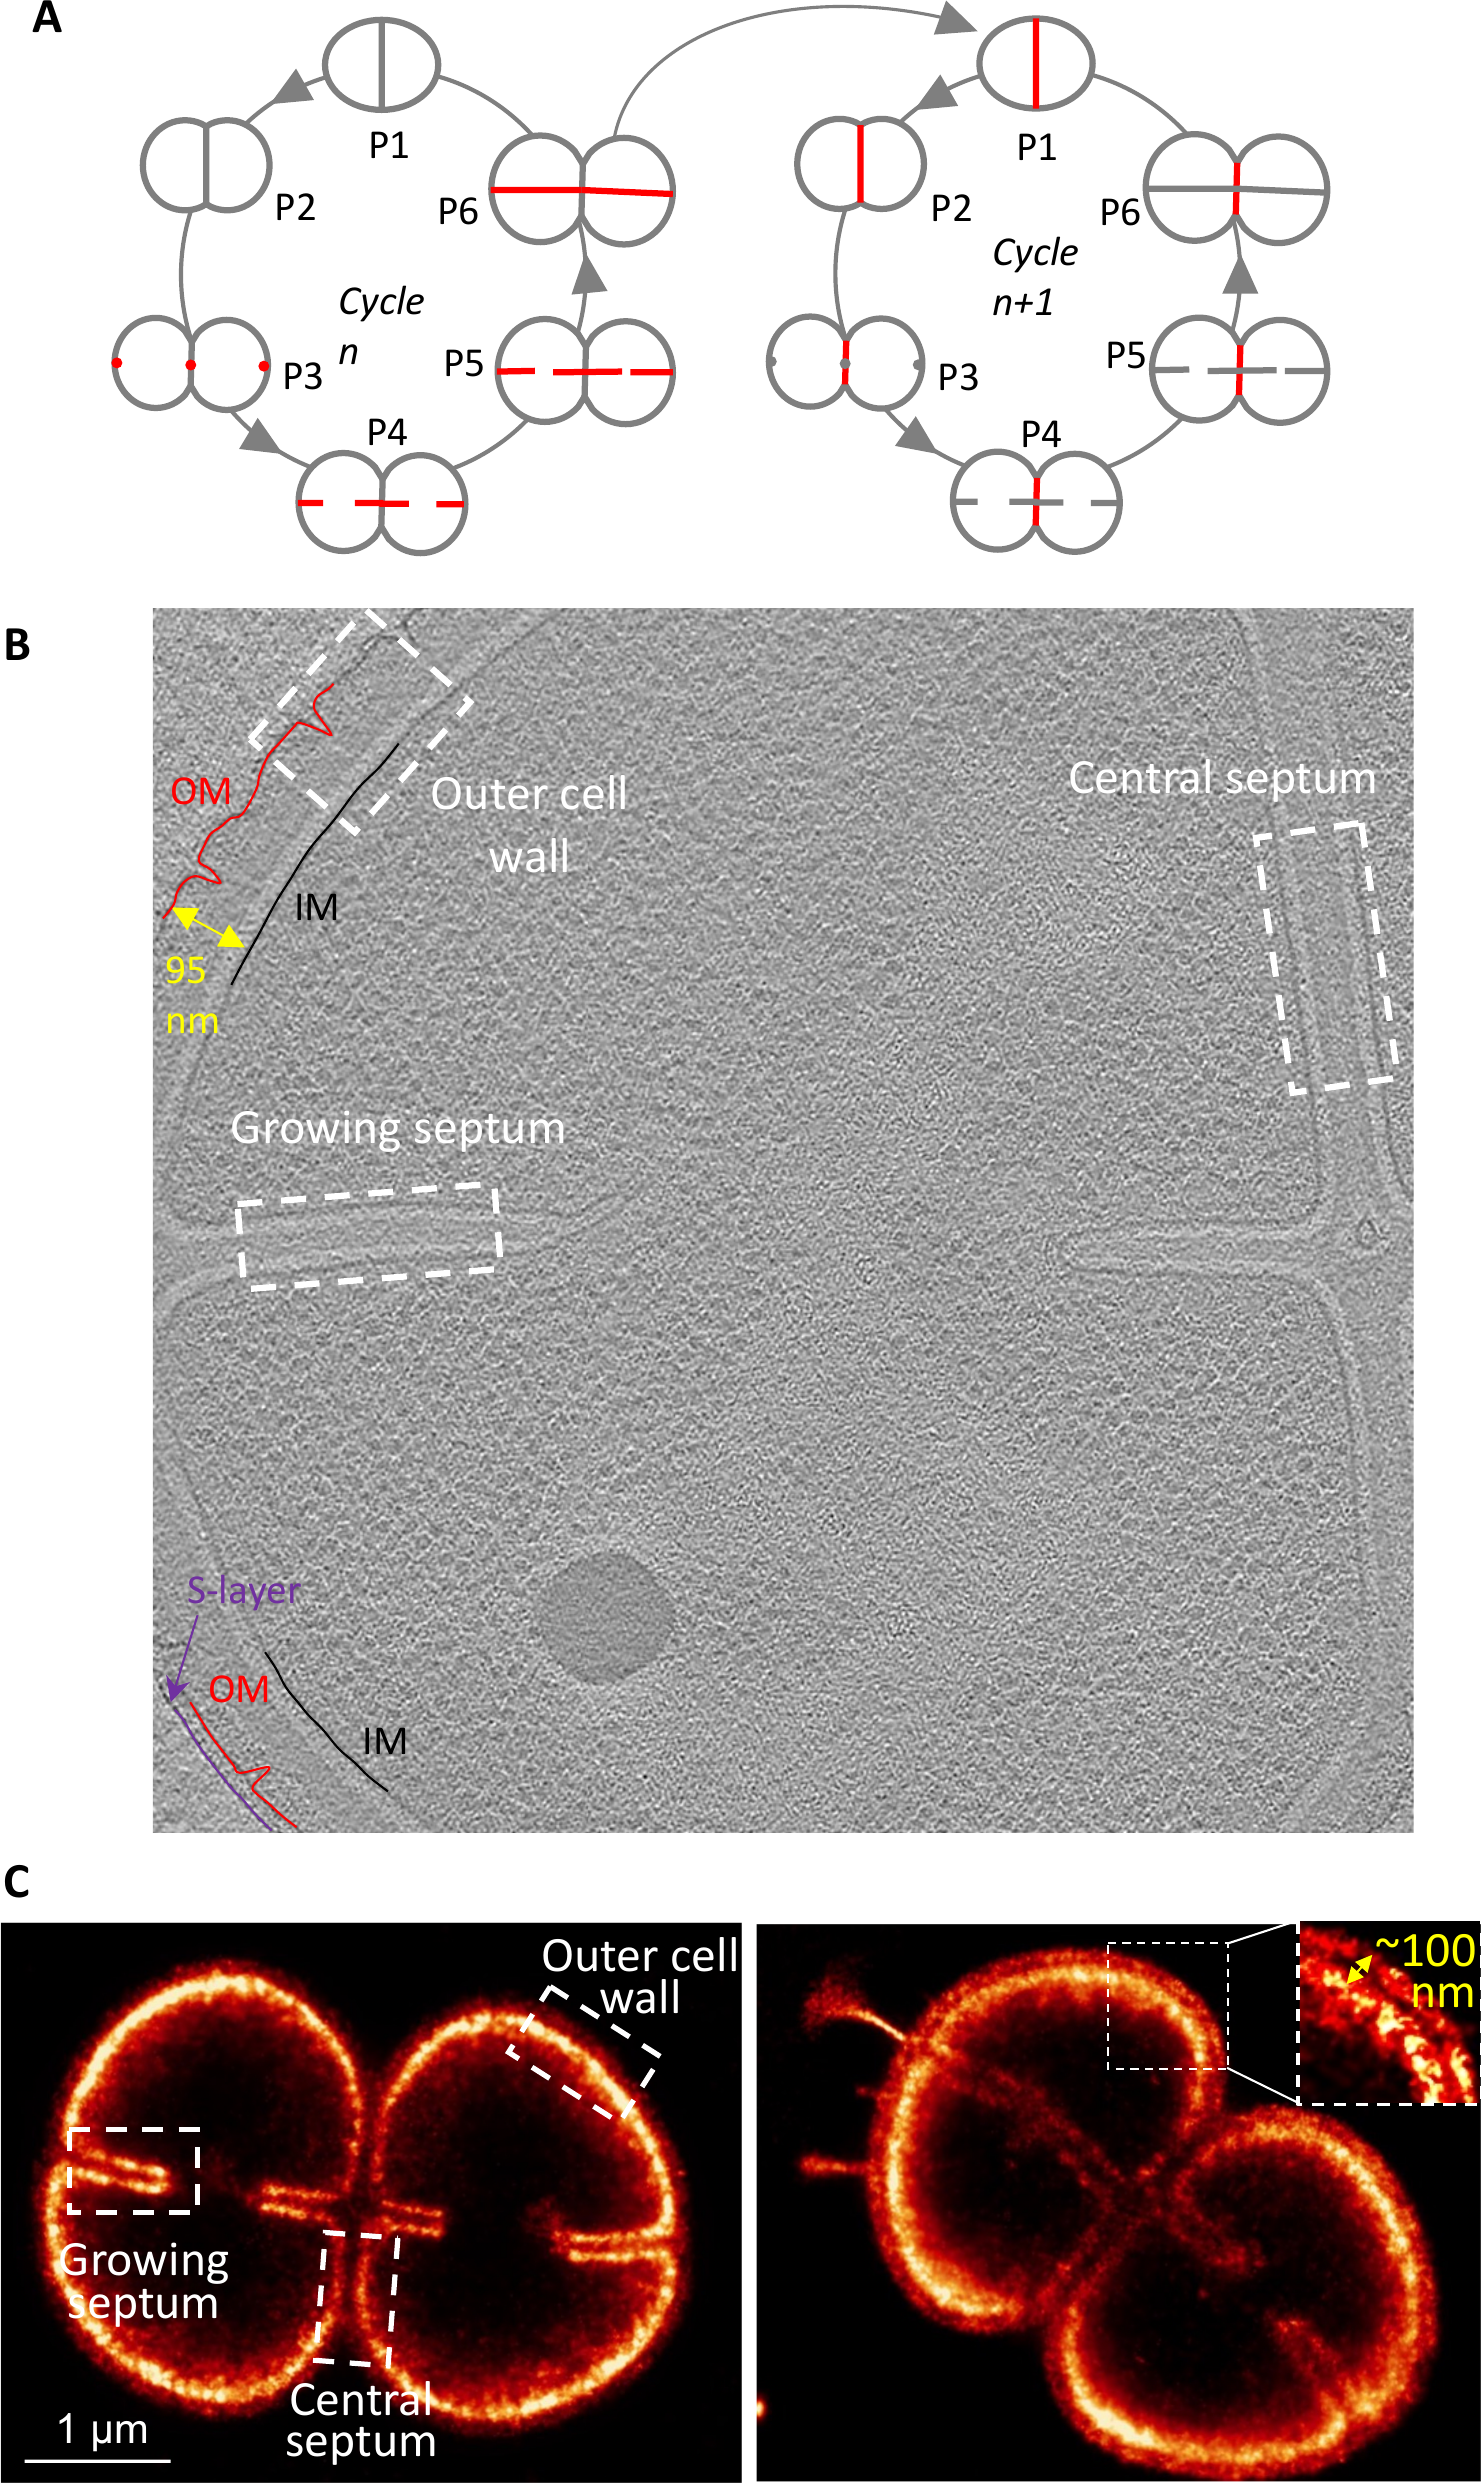
\includegraphics[width=\textwidth]{drad_paper/fig1.png}
    \caption{TODO}
    \label{drad_fig1}
\end{figure}

The outer cell wall bears two lipid bilayers that can be seen as dark lines in the cryo-ET data and could be distinguished on a few occasions in our super-resolved PAINT images of Nile Red stained \textit{D. radiodurans} (\autoref{drad_fig1}B, right panel).
With both techniques, the distance between the inner (IM) and outer (OM) cell membranes was in good agreement and was found to be around \qty{95}{nm} (\autoref{drad_fig1}).
A more in-depth analysis of the cell wall layer composition was facilitated by the preparation of straightened cell wall projections of the cryo-ET images using a recently developed tool, blik~\cite{gaifasBlikExtensible3D2024}.
Density profiles of the outer cell wall revealed that this region was composed of 6 distinct layers: (i) an inner plasma membrane, (ii) a low-density periplasmic region, (iii) a high-density PG layer, (iv) an intermediate layer previously described as the SlpA layer~\cite{vonkugelgenMultidomainConnectorLinks2022}, (v) an outer plasma membrane and (vi) a discontinuous hexagonally packed S-layer on the outer surface of the bacteria (\autoref{drad_fig2}A).
A distinctive white line was seen to separate the PG layer from the SlpA layer and V-shaped invaginations of the outer plasma membrane were seen regularly along this outer cell wall.
Measurements made on numerous cryo-ET datasets allowed us to determine the mean thickness of each of these 6 layers.
When present, the S-layer was typically located at \qty{18}{nm} above the outer cell membrane, the SlpA layer was found to be \qty{34.5}{nm} in thickness in good agreement with the estimated dimensions of the SlpA complex that stretches across this layer~\cite{vonkugelgenMultidomainConnectorLinks2022}.
The PG layer was found to be \sim\qty{42.5}{nm} in thickness and located \sim\qty{15.5}{nm} above the inner membrane with a low-density region located in between these two essential layers.
Interestingly, these measurements revealed that the inner membrane bilayer was significantly thicker than the outer plasma membrane (\qty{5.5}{nm} vs \qty{4.0}{nm}) suggesting distinct lipid compositions.

\begin{figure}[ht]
    \centering
    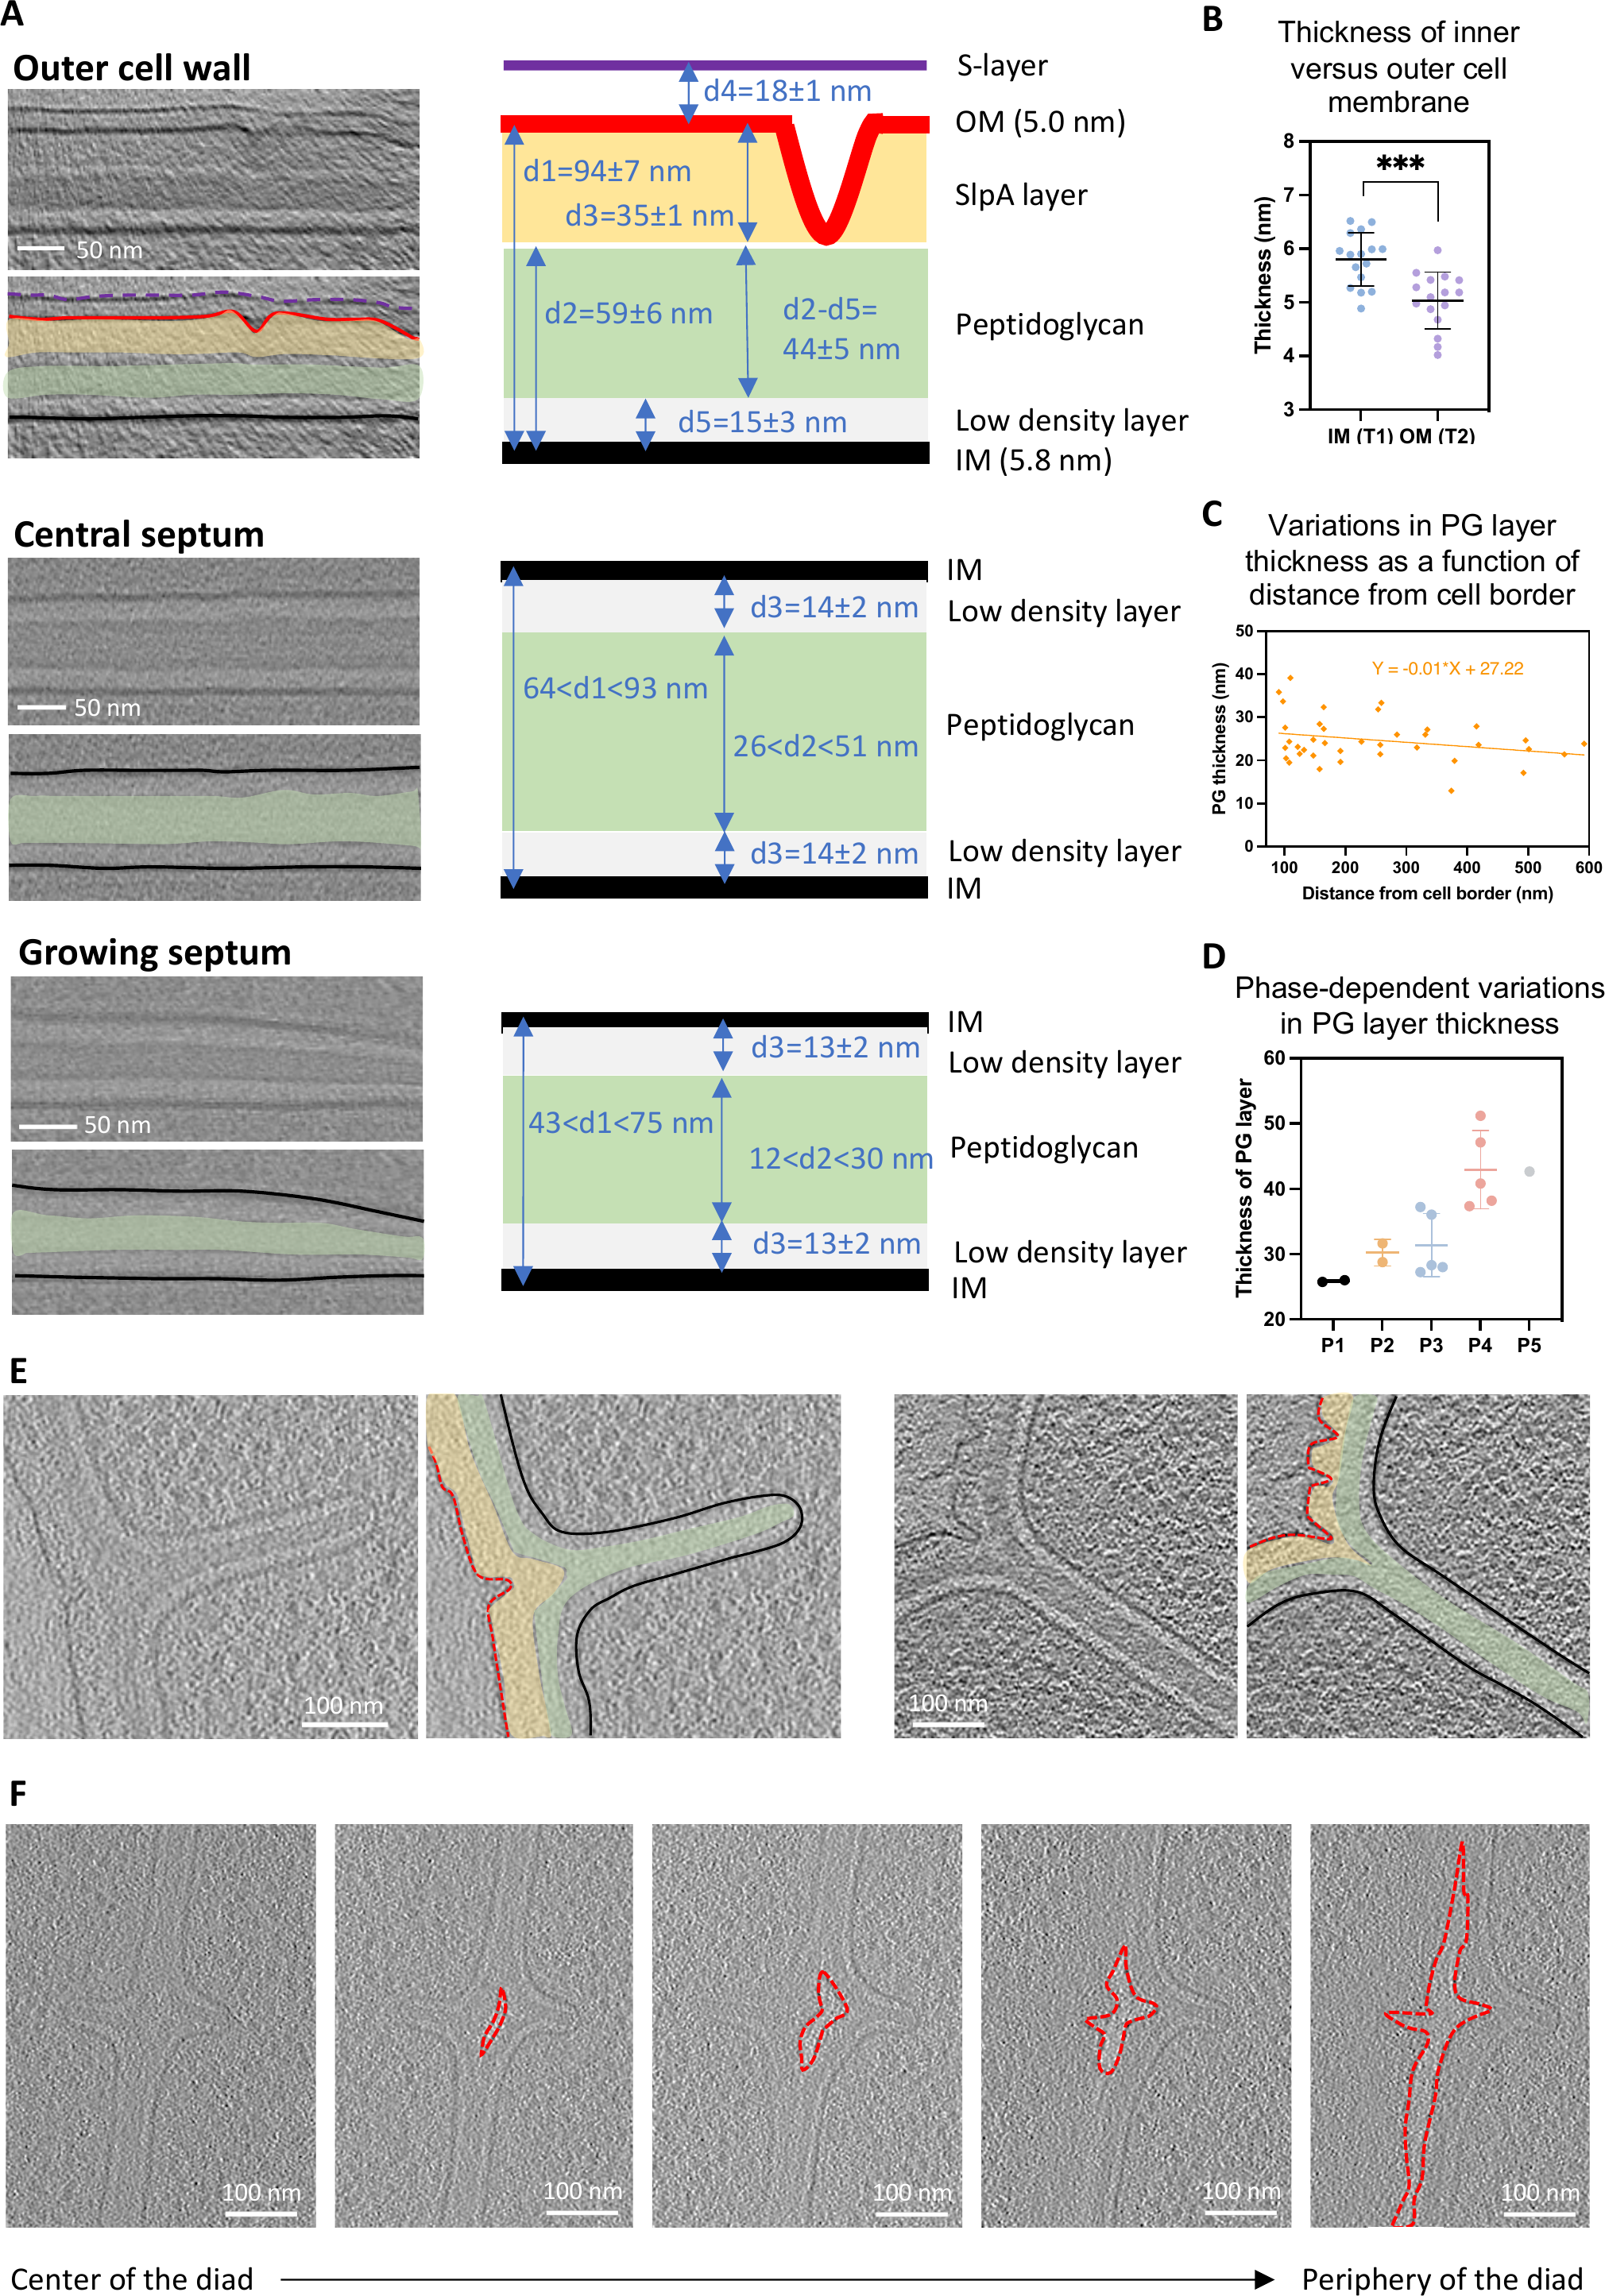
\includegraphics[width=\textwidth]{drad_paper/fig2.png}
    \caption{TODO}
    \label{drad_fig2}
\end{figure}

A similar procedure was used to analyse the composition of the growing septa and the central cell wall region.
The outer layers of the external cell wall were missing in these regions, notably the S-layer, the outer membrane bilayer and the SlpA layer, and instead they were composed of only the inner plasma membrane, the low-density periplasmic region and the PG layer (\autoref{drad_fig2}A).
In contrast to the inner membrane and low-density layers that showed similar thickness in these two locations, the PG layer displayed significant variations, ranging from \qty{42}{nm} to \qty{56}{nm} in the central cell wall and as low as \qty{35}{nm} in the growing septa.
In both the growing septa and the central cell wall, the PG layer was typically thicker at the cell periphery than at the tip of the septum or the centre of the diad respectively, and in the central cell wall, the mean thickness of the PG layer was also found to vary substantially as a function of the phase of the cell cycle, suggesting a progressive thickening of this layer until reaching its definite size prior to the splitting of the diad into two cells (\autoref{drad_fig2}A).

At the junction between the outer cell wall and the growing septum (\autoref{drad_fig2}B and \autoref{drad_sfig2} for more examples), we observed that the PG and low-density periplasmic layers followed the inner membrane, while the outer layers (SlpA layer and outer membrane) were restricted to the outer cell wall.
V-shaped invaginations in the outer membrane were often observed at these junctions and were found to extend inwards during the splitting of the two daughter cells during the subsequent division cycle.
As shown in \autoref{drad_fig2}C, cell splitting is a progressive process, most likely initiated from the cell periphery and moving inwards from both sides of the cell towards the center of the diad forming bubble-like membrane structures (\autoref{drad_sfig1}B for more examples).
Splitting occurs concomitantly with the addition of the SlpA layer and finally the outer cell membrane to the central septum cell wall to protect the cells from the external environment (\autoref{drad_fig2}C).

\FloatBarrier

\subsection{Structure of septal tips}

A close inspection of the tomograms revealed that the tips of the growing septa exhibited particular structures.
A majority of septa (40 of the 64 septa visible in our tomograms) were slightly tapered at their tips and the low-density periplasmic region was significantly thinner in these regions bringing the PG layer very close to (in some cases even touching) the inner membrane (\autoref{drad_fig3}A).
Strikingly, in nearly 40\% of the observed septa, membrane protrusions, reported in earlier studies as mesosomes~\cite{thornleyFineStructureMicrococcus1965,sleytrStudyFreezeetchingFine1973}, were observed at the tips of growing septa (\autoref{drad_fig3}B-C and \autoref{drad_sfig2} for more examples).
These structures are composed solely of the low-density layer and are delimited by the inner membrane.
They were in a large majority of cases observed in cells in early stages of the septation process bearing short septa.
These extensions were found to adopt either extended tube-like structures or more circular loop-like structures.
In all cases, they appeared to be very flexible, probably as a result of the absence of a PG layer to rigidify the extension.
This intrinsic flexibility may explain why the tips of the growing septa were often not observed in the super-resolved images of Nile Red-labelled \textit{D. radiodurans} cells (\autoref{drad_fig3}C, left panel).
Instead, in these images, open ends were observed at the septal tips, suggesting that either the Nile Red dye poorly labelled these highly curved membrane bilayers or that the tips were very mobile and not captured in live imaging experiments.
Both of these phenomena may also be at play.
On a few occasions, we did observe more poorly defined Nile Red labelling at the tips of growing septa that may correspond to these flexible membrane protrusions (\autoref{drad_fig3}C, right panel).

\begin{figure}[ht]
    \centering
    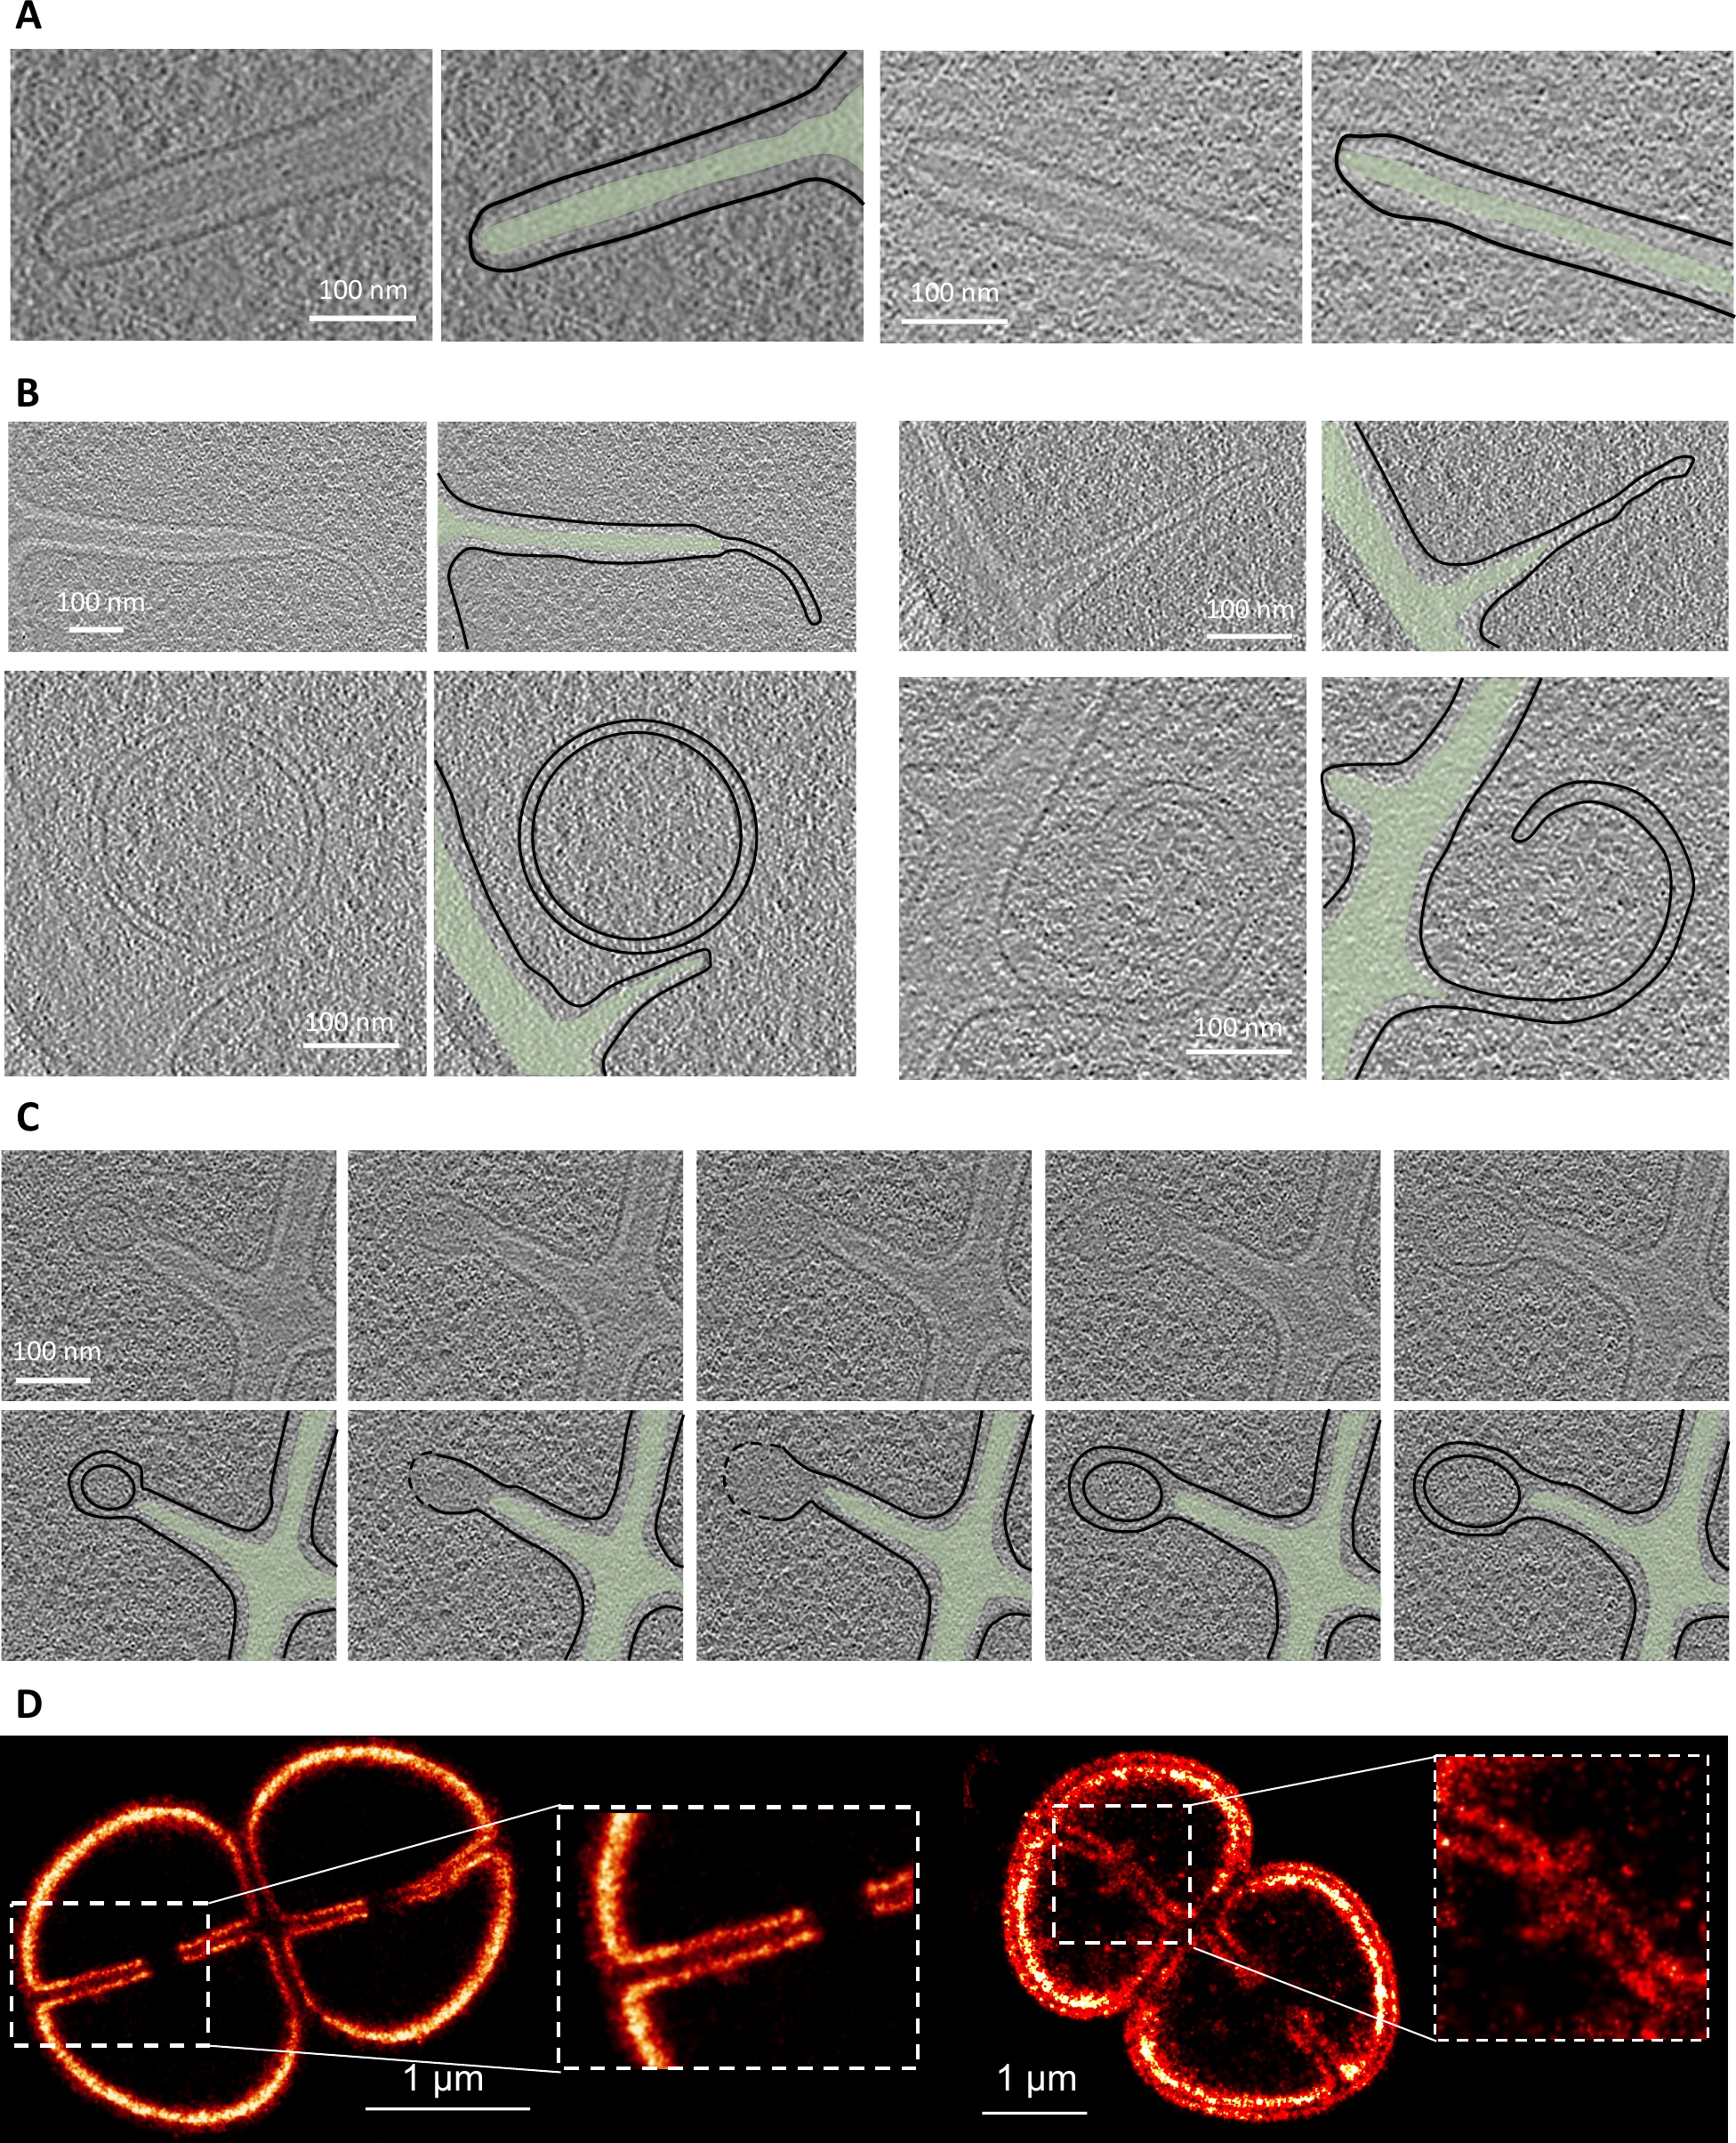
\includegraphics[width=\textwidth]{drad_paper/fig3.png}
    \caption{TODO}
    \label{drad_fig3}
\end{figure}

\FloatBarrier

\subsection{Septation through a "sliding door" mechanism}

Using timelapse 3D video confocal microscopy of Nile Red stained \textit{D. radiodurans} bacteria immobilized in various orientations on agarose pads (\autoref{drad_sfig3}), we followed the division process in live cells (SI videos 1 and 2).
Septation was found to involve several steps.
First, two septa originating from opposite sides of the cell grow inwards with a flat leading edge creating a central gap stretching from the top to the bottom of the cell.
As the septa grow, the leading edge progressively becomes more curved forming a cat's eye structure in between the two opposite septa.
Finally, when the two septa come close to each other, fusion starts first at the top and bottom of the cell and then rapidly proceeds through a zipping mechanism from the cell periphery to the cell center.
3D PAINT images of Nile Red labelled \textit{D. radiodurans} cells confirmed these observations, allowing to capture high-resolution images of dividing cells exhibiting septa with flat or slightly curved leading edges embracing a central gap that stretches all across the cell (\autoref{drad_fig4}A).
Kymographs of individual septation events were extracted from the live cell confocal acquisitions to probe the kinetics of this process (\autoref{drad_fig4}B).
These revealed that septation is a linear process in which the external and internal septa grow respectively at rates of \qty{7.3(0.5)}{nm.min^{-1}}  and \qty{4.1(0.7)}{nm.min^{-1}} until full closure.
Interestingly, the external septum starts growing ahead of the internal septum, as can be seen from the asymmetric V-shaped structure of the kymographs, and grows at a faster rate than the internal septum (\autoref{drad_fig4}B).
This may be explained by the fact that the external septum needs to grow further than the internal septum to reach the site of fusion located at mid-cell and has to compensate for the expansion of the cells that is occurring simultaneously (\autoref{drad_fig4}A).
A flat leading edge and an asymmetric growth of the external and internal septa were also observed in our cryo-ET data, which captured bacteria at various stages of the division process (\autoref{drad_fig4}C-D).

\begin{figure}[ht]
    \centering
    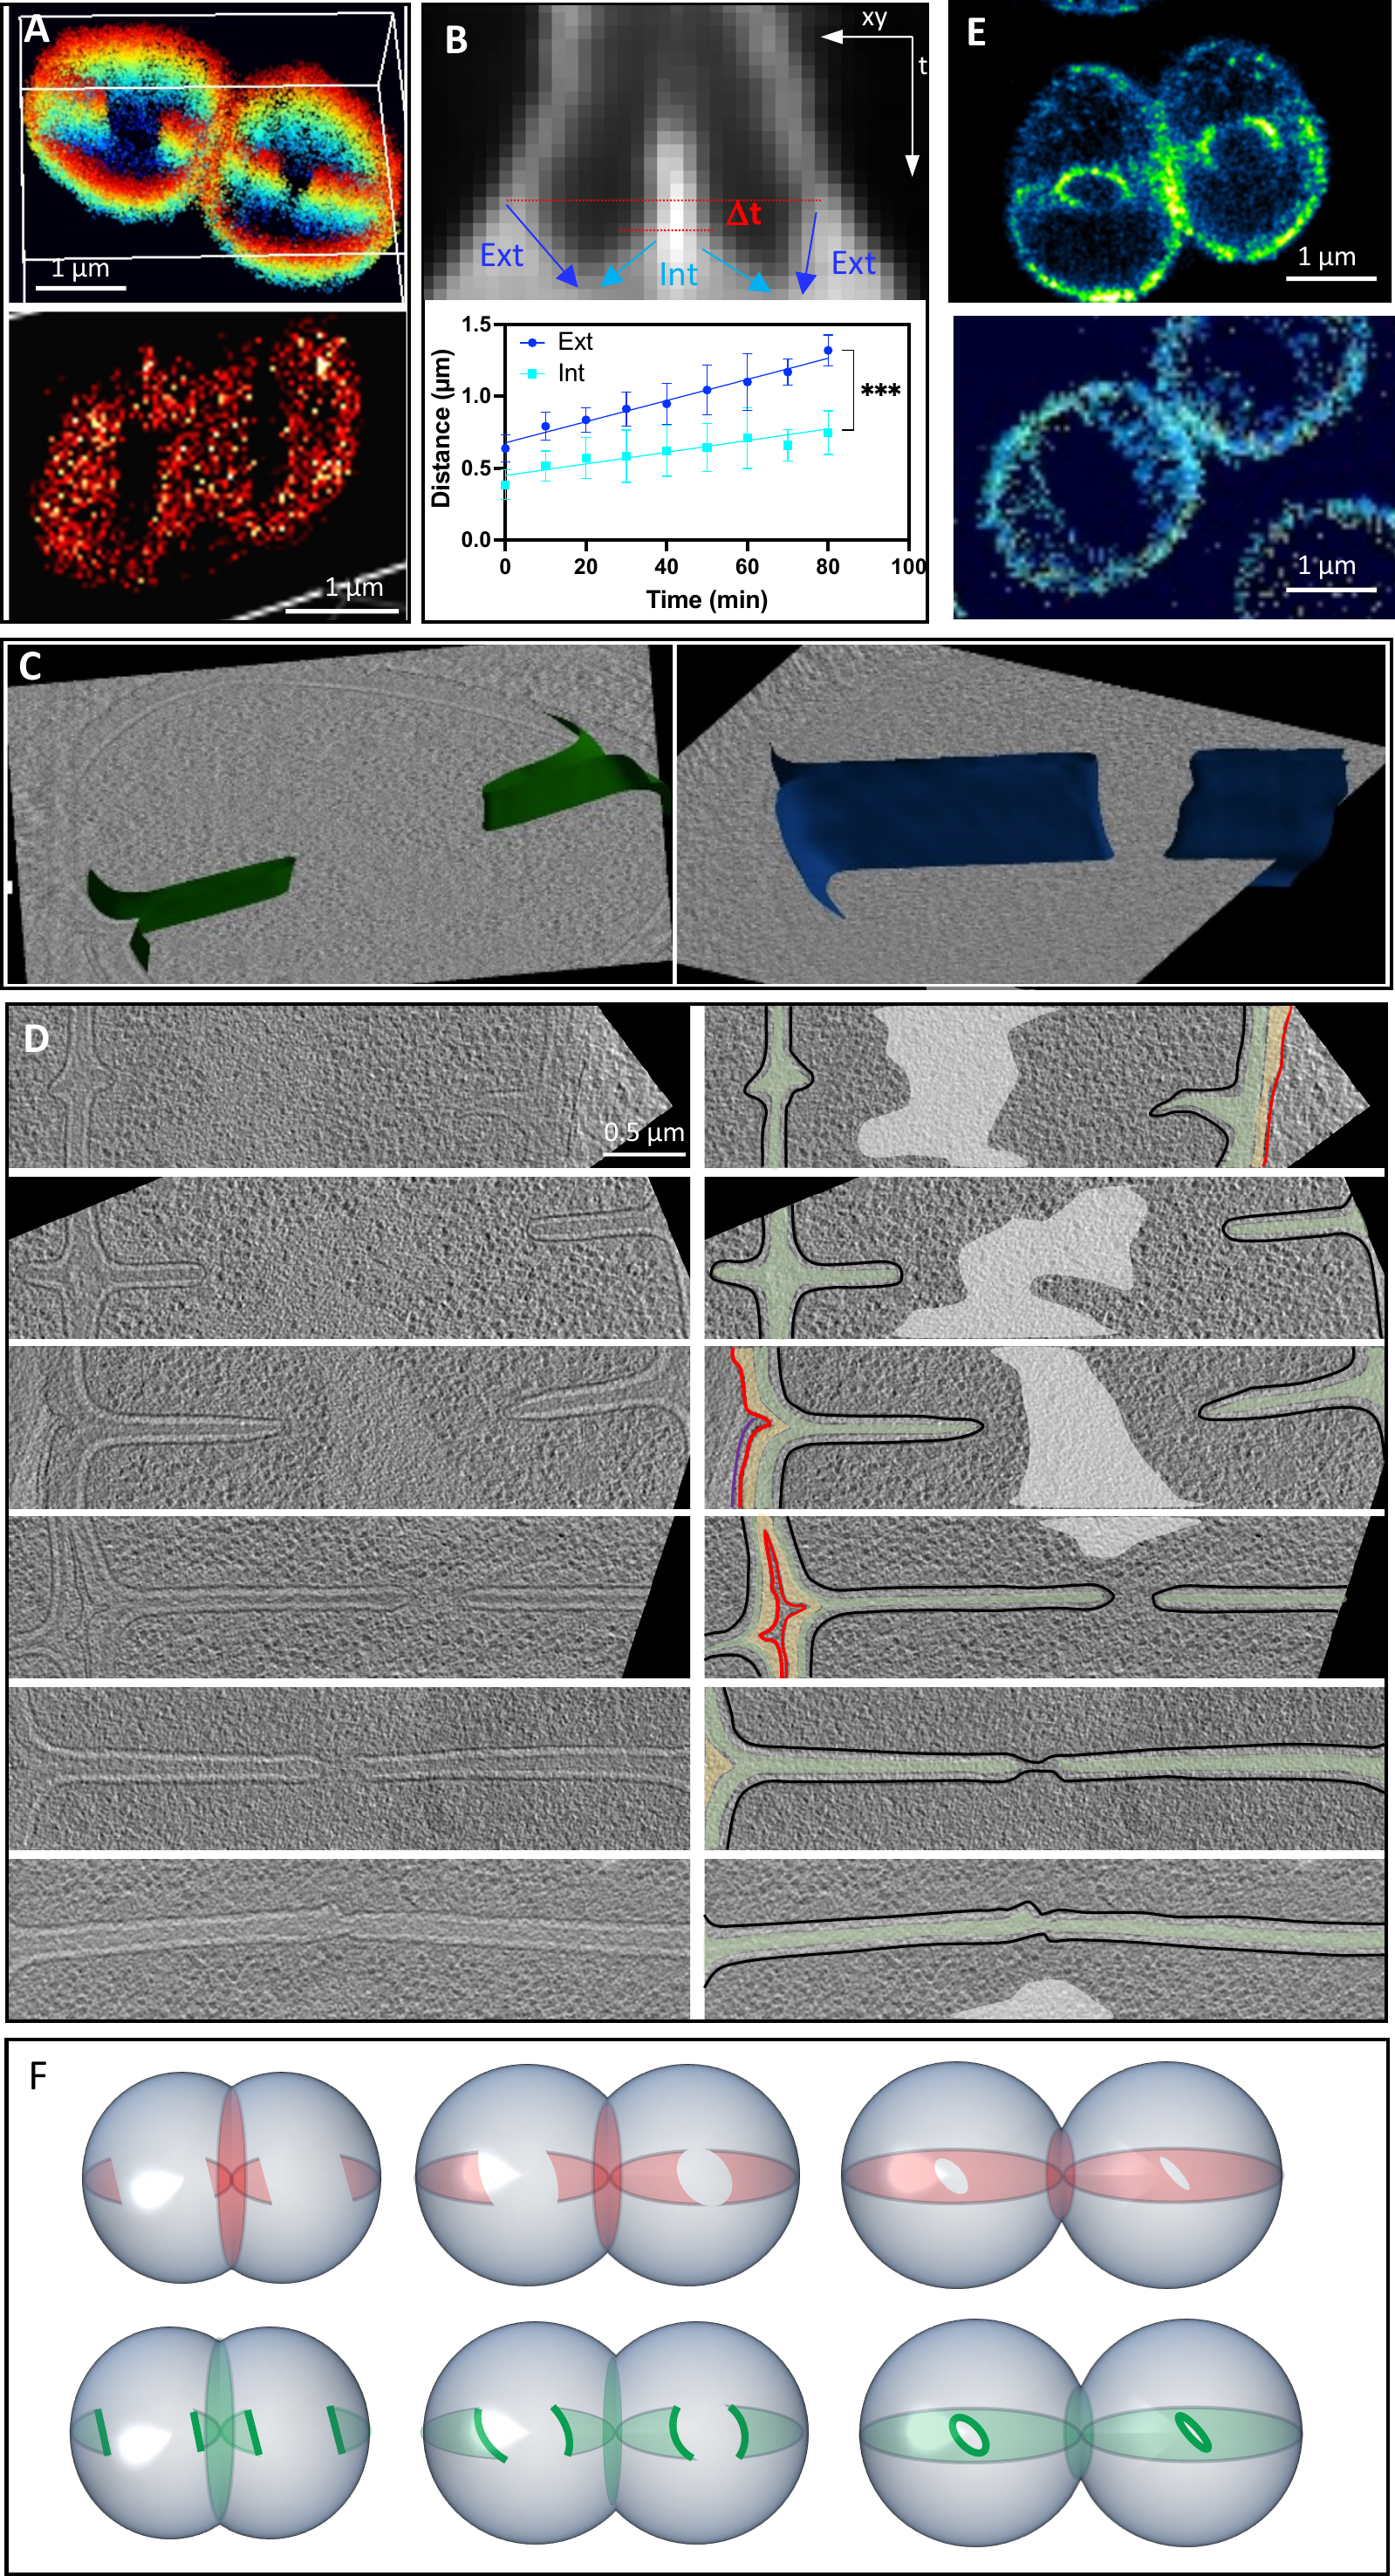
\includegraphics[width=.7\textwidth]{drad_paper/fig4.png}
    \caption{TODO}
    \label{drad_fig4}
\end{figure}

In addition to staining the cell membrane, we also labelled the PG layer of \textit{D. radiodurans} cell walls by incorporating modified D-alanine (zDA) into the cell wall that was subsequently labelled by click chemistry with fluorescent probes suitable for either confocal or dSTORM microscopy (\autoref{drad_sfig4}).
The PG labelling pattern (\autoref{drad_fig4}E and \autoref{drad_sfig5}) was very similar to that of Nile Red labelled cells, with an efficient incorporation occurring in all regions of the cell wall (septal, central and outer cell walls).
The main difference was that the PG labelling was more prominent at the leading edge of the growing septa than elsewhere, suggesting this likely corresponds to the major site of active PG synthesis in these dividing cells (\autoref{drad_fig4}F).
This is particularly visible at late stages of the cell cycle, either just before (Phase 5) or just after cytokinesis (Phase 6), where an intense band of labelled PG can be seen at the site of fusion where the two opposing septa meet (\autoref{drad_sfig5}C).
In agreement with these observations, pulse-chase experiments in which bacteria were returned to the incubator for 45 minutes (chase) after incorporation of the modified D-Alanine (pulse) into their cell walls, revealed that septa having incorporated zDA labelling at their tips during the pulse period, were progressively extended further by unlabelled PG, indicating that new PG is added to the existing layer in an inwards direction until the opposing septa are close enough to fuse (\autoref{drad_fig4}F and \autoref{drad_sfig6}).

Close examination of the tomograms also revealed that the position and shape of the growing septa changed as a function of their length (\autoref{drad_fig4}D).
At early stages of the septation process, short septa were not always precisely facing each other and their tips were often bent and bearing membrane extensions, while at later stages, septa were remarkably straight and fully aligned to ensure fusion of the septa originating from opposite sides of the cell.
The presence of a PG layer in the growing septa appears to be a pre-requisite for the formation of these straight and well-aligned septa, indicating that the synthesis of the PG layer may provide the necessary rigidity to the growing cell walls for the final closure.
This final fusion step was captured in two of the tomograms and was found to proceed first through fusion of the lipid bilayers (highlighted in red in \autoref{drad_fig4}D) and subsequently through synthesis of PG to fill the gap and "glue" the two septa together.
Taken together, these data allow us to propose a model for septation through the "sliding doors" mechanism, which is illustrated schematically in \autoref{drad_fig4}F.

\FloatBarrier

\subsection{PG synthesis in the outer cell wall and in the septa are performed by distinct machineries}

To better understand the molecular mechanisms underlying this unusual mode of septation, we treated \textit{D. radiodurans} cultures with the \beta-lactam antibiotic, ampicillin, and compared the growth of untreated and treated Nile Red labelled cells by 3D confocal timelapse microscopy for a three-hour period (SI videos 3 and 4).
Ampicillin is known to bind to the active sites of certain PBPs, thereby inhibiting their enzymatic cell wall synthesis function~\cite{sauvageGlycosyltransferasesTranspeptidasesPenicillinBinding2016}.
To our surprise, septation but not cell growth was arrested by ampicillin treatment (\autoref{drad_fig5}).
Indeed, the growth of the outer cell perimeter was unaffected by this treatment during this three-hour period, while growth of both the internal and external septa were rapidly arrested (\autoref{drad_fig5}B-C).
After 1 hour, the septa even started to shorten, suggesting they may be undergoing disassembly and degradation (\autoref{drad_fig5}C).
As a result of this change in the balance between cell growth and septation, cells progressively became distorted (more elongated with a slight bulge at sites of division) as evidenced by the substantially increased diameter (d) to perimeter (p) ratio after three hours of treatment with ampicillin (\autoref{drad_fig5}D).
The specific inhibition of septal growth by ampicillin suggests that the PBPs responsible for PG synthesis and maturation in the septa are distinct from those involved in outer cell wall growth.

\begin{figure}[ht]
    \centering
    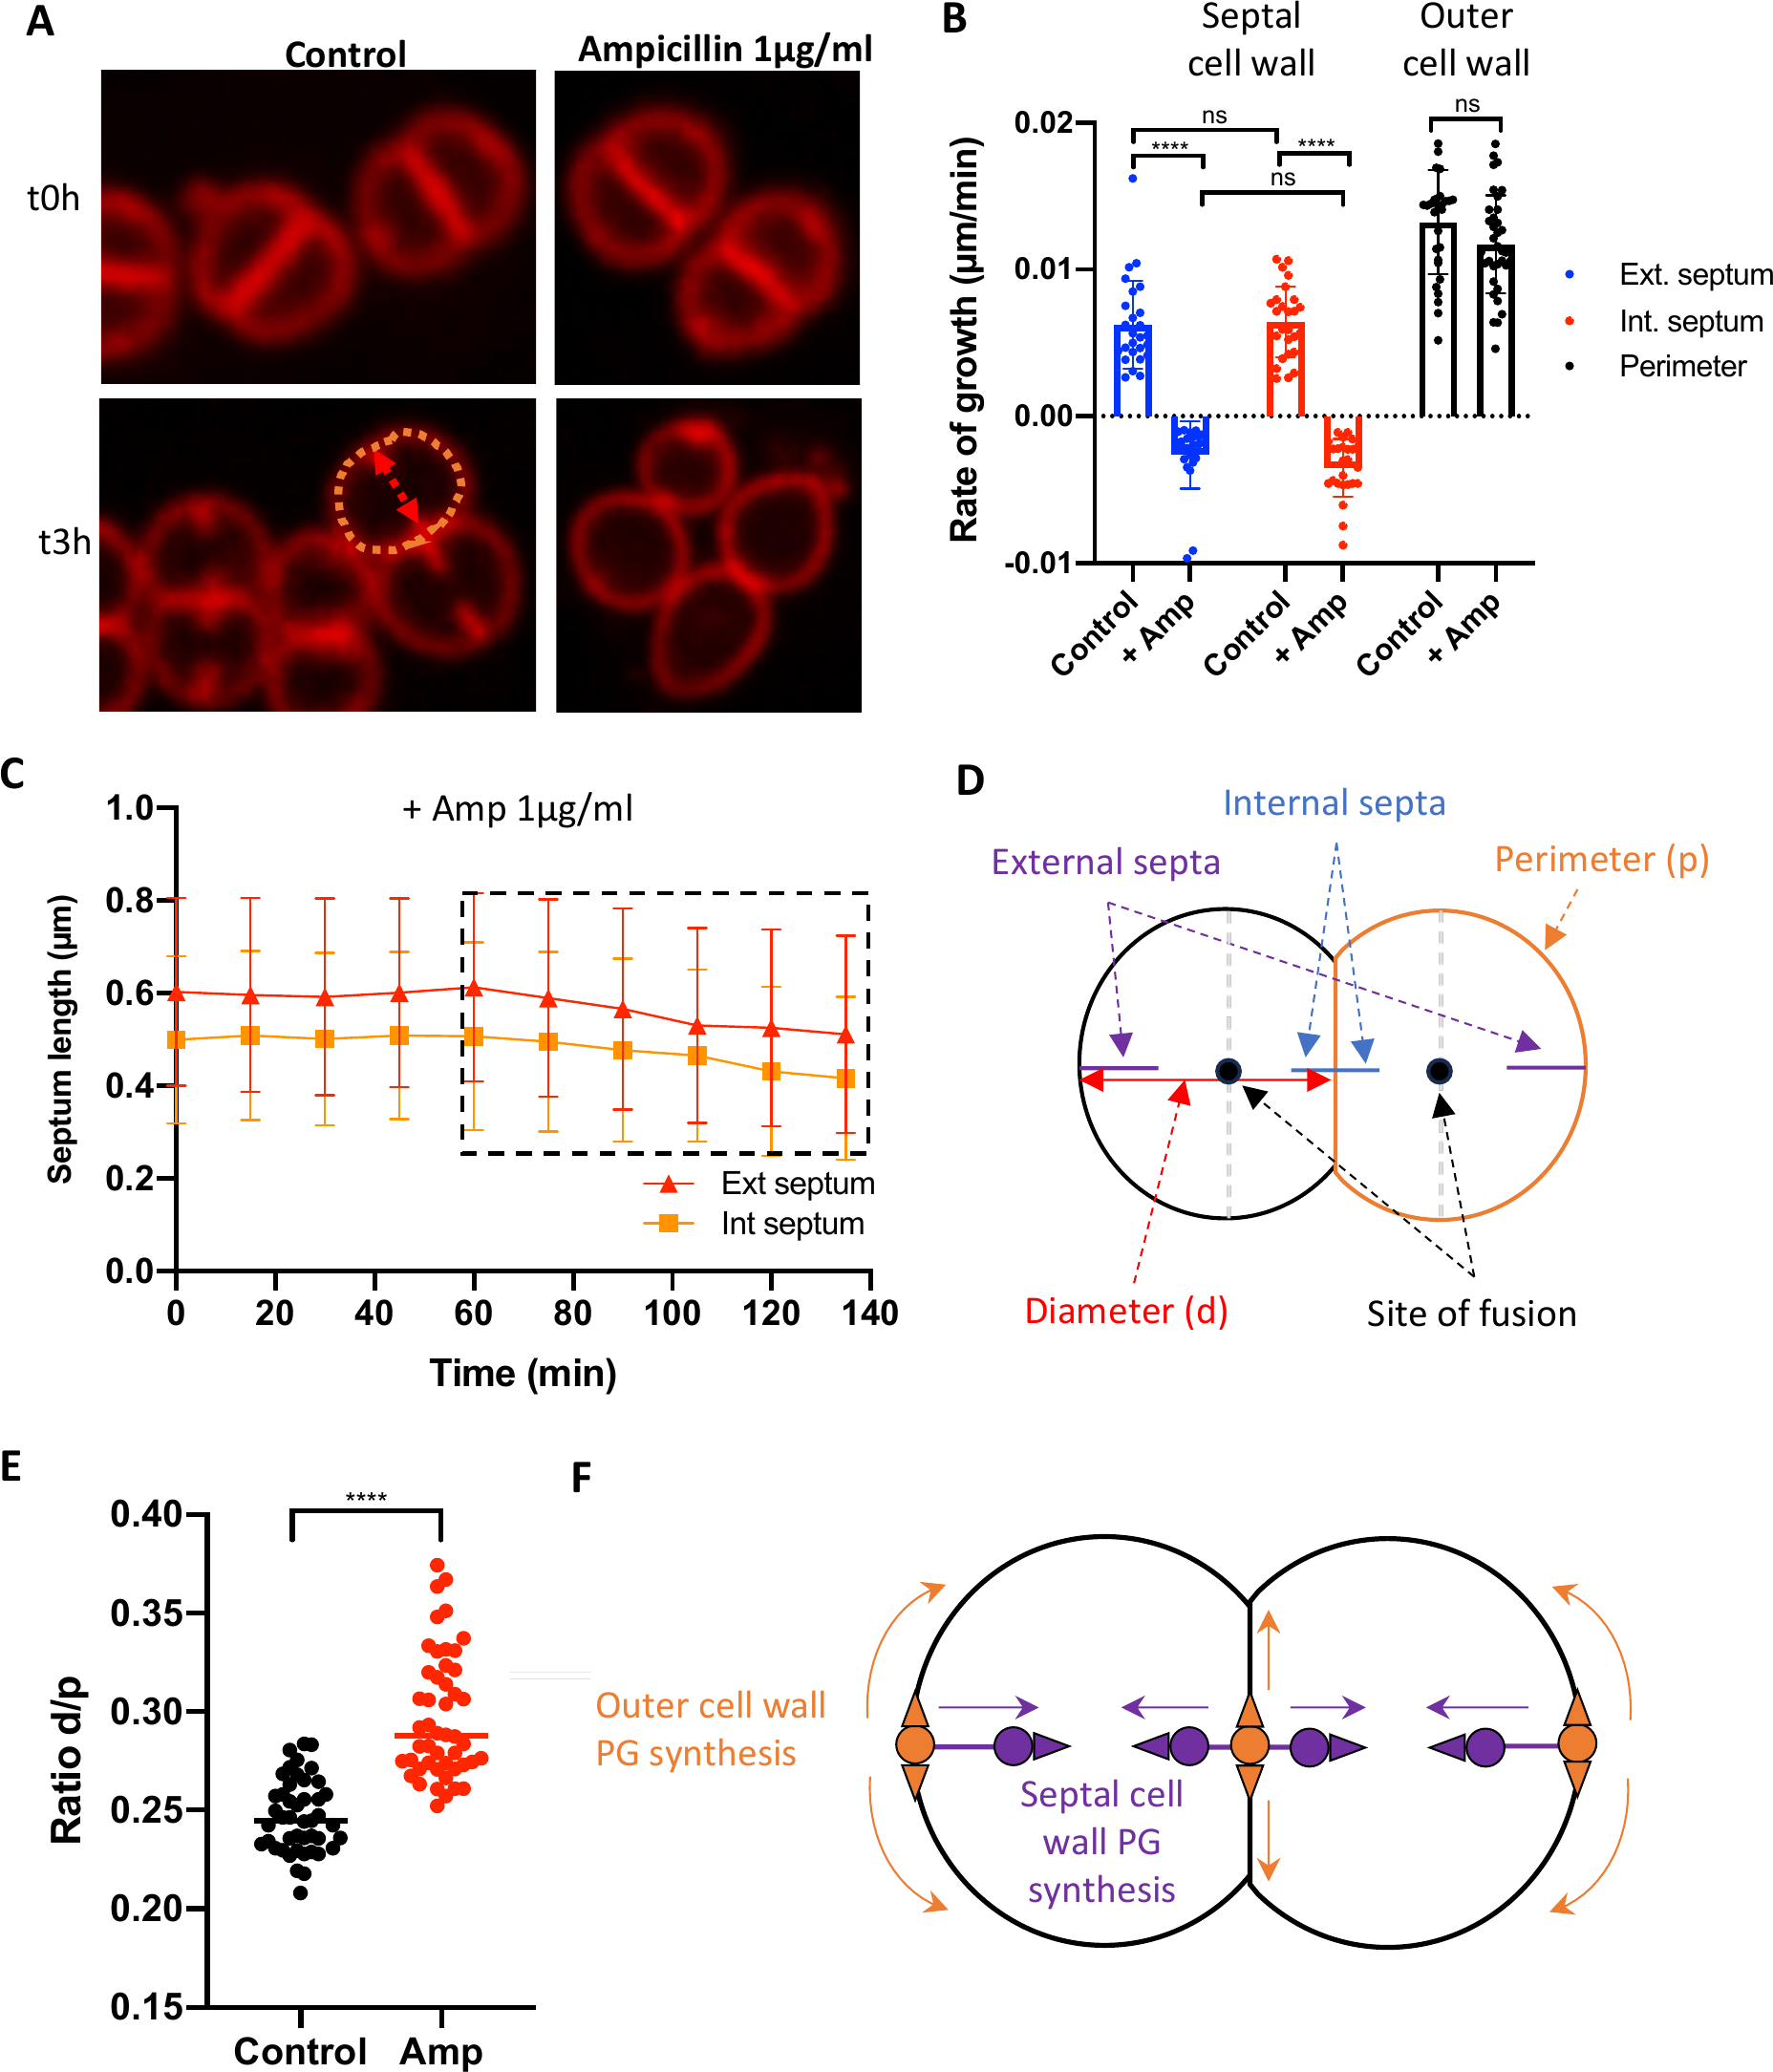
\includegraphics[width=.8\textwidth]{drad_paper/fig5.png}
    \caption{TODO}
    \label{drad_fig5}
\end{figure}

Next, we repeated the zDA incorporation experiment on cells pre-grown for either 1 or 2h in the presence of ampicillin before the labelling (\autoref{drad_sfig7}).
In these conditions, zDA was still readily incorporated into the outer cell wall, as expected based on our timelapse experiments.
In contrast, no labelling was seen in the septal regions except at sites of septation initiation, where a distinctive bright PG-labelled ring was observed (\autoref{drad_sfig7}).
These rings were occasionally seen in untreated cells (\autoref{drad_sfig_missing}), but were much more abundant in ampicillin-treated cells and in particular in samples pre-grown for 2 hours in the presence of the \beta-lactam antibiotic, where approximately 50\% of the cells displayed such ring-shaped PG labelling (\autoref{drad_sfig7}B).
The initial PG synthesis at the start of septation thus appears to be unaffected by ampicillin, while subsequent growth and extension of the septa is fully arrested by this treatment.
A shared PG machinery located at the junction between the outer cell wall and the start of septation may therefore be involved in both outer cell wall synthesis and initiation of septation, but a distinct set of proteins likely located at the tip of the growing septa appear to be responsible for PG synthesis across the dividing cells (\autoref{drad_fig5}E).
This finding is supported also by the pulse-chase experiments (\autoref{drad_sfig6}) in which we observed that most of the labelling of the septal regions, but not of the outer cell walls was lost after the chase period, indicating that the PG structure and/or maturation process are quite distinct in these two types of cell wall.

\FloatBarrier

\subsection{FtsZ is present at the tips of septa}\label{drad_ftsz}

We investigated the location of FtsZ, one of the key players in bacterial cell division, in dividing \textit{D. radiodurans} cells using both fluorescence microscopy and cryo-ET.
Two strategies were used to label FtsZ: (i) immunolabelling of an endogenously HA-tagged FtsZ or (ii) endogenous tagging of FtsZ with a photoconvertible fluorescent protein, mEos4B.
The latter was compatible with live cell imaging, but this genetically modified strain of \textit{D. radiodurans} showed altered cell morphology (forming many large cells with likely impaired septation) and only a small fraction of cells exhibited fluorescence signal and visible Z-rings (\autoref{drad_fig6}A).
In contrast, the strain expressing HA-tagged FtsZ grew very well with no obvious morphological defects and FtsZ could be detected after fixing and permeabilizing the cells with an anti-HA antibody by either confocal or dSTORM microscopy (\autoref{drad_fig6}A-B).
Both strategies indicated that \textit{D. radiodurans} FtsZ forms ring- or oval-shaped structures of various sizes as reported for other bacteria, some of which appear to be incomplete.
Dual labelling of FtsZ and the cell membrane also revealed that FtsZ locates to the tip of growing septa at all stages of septation, including very early stages when septa are not yet visible by fluorescence microscopy (\autoref{drad_fig6}B).
At these early stages, FtsZ appeared to form arches rather than complete rings.

\begin{figure}[ht]
    \centering
    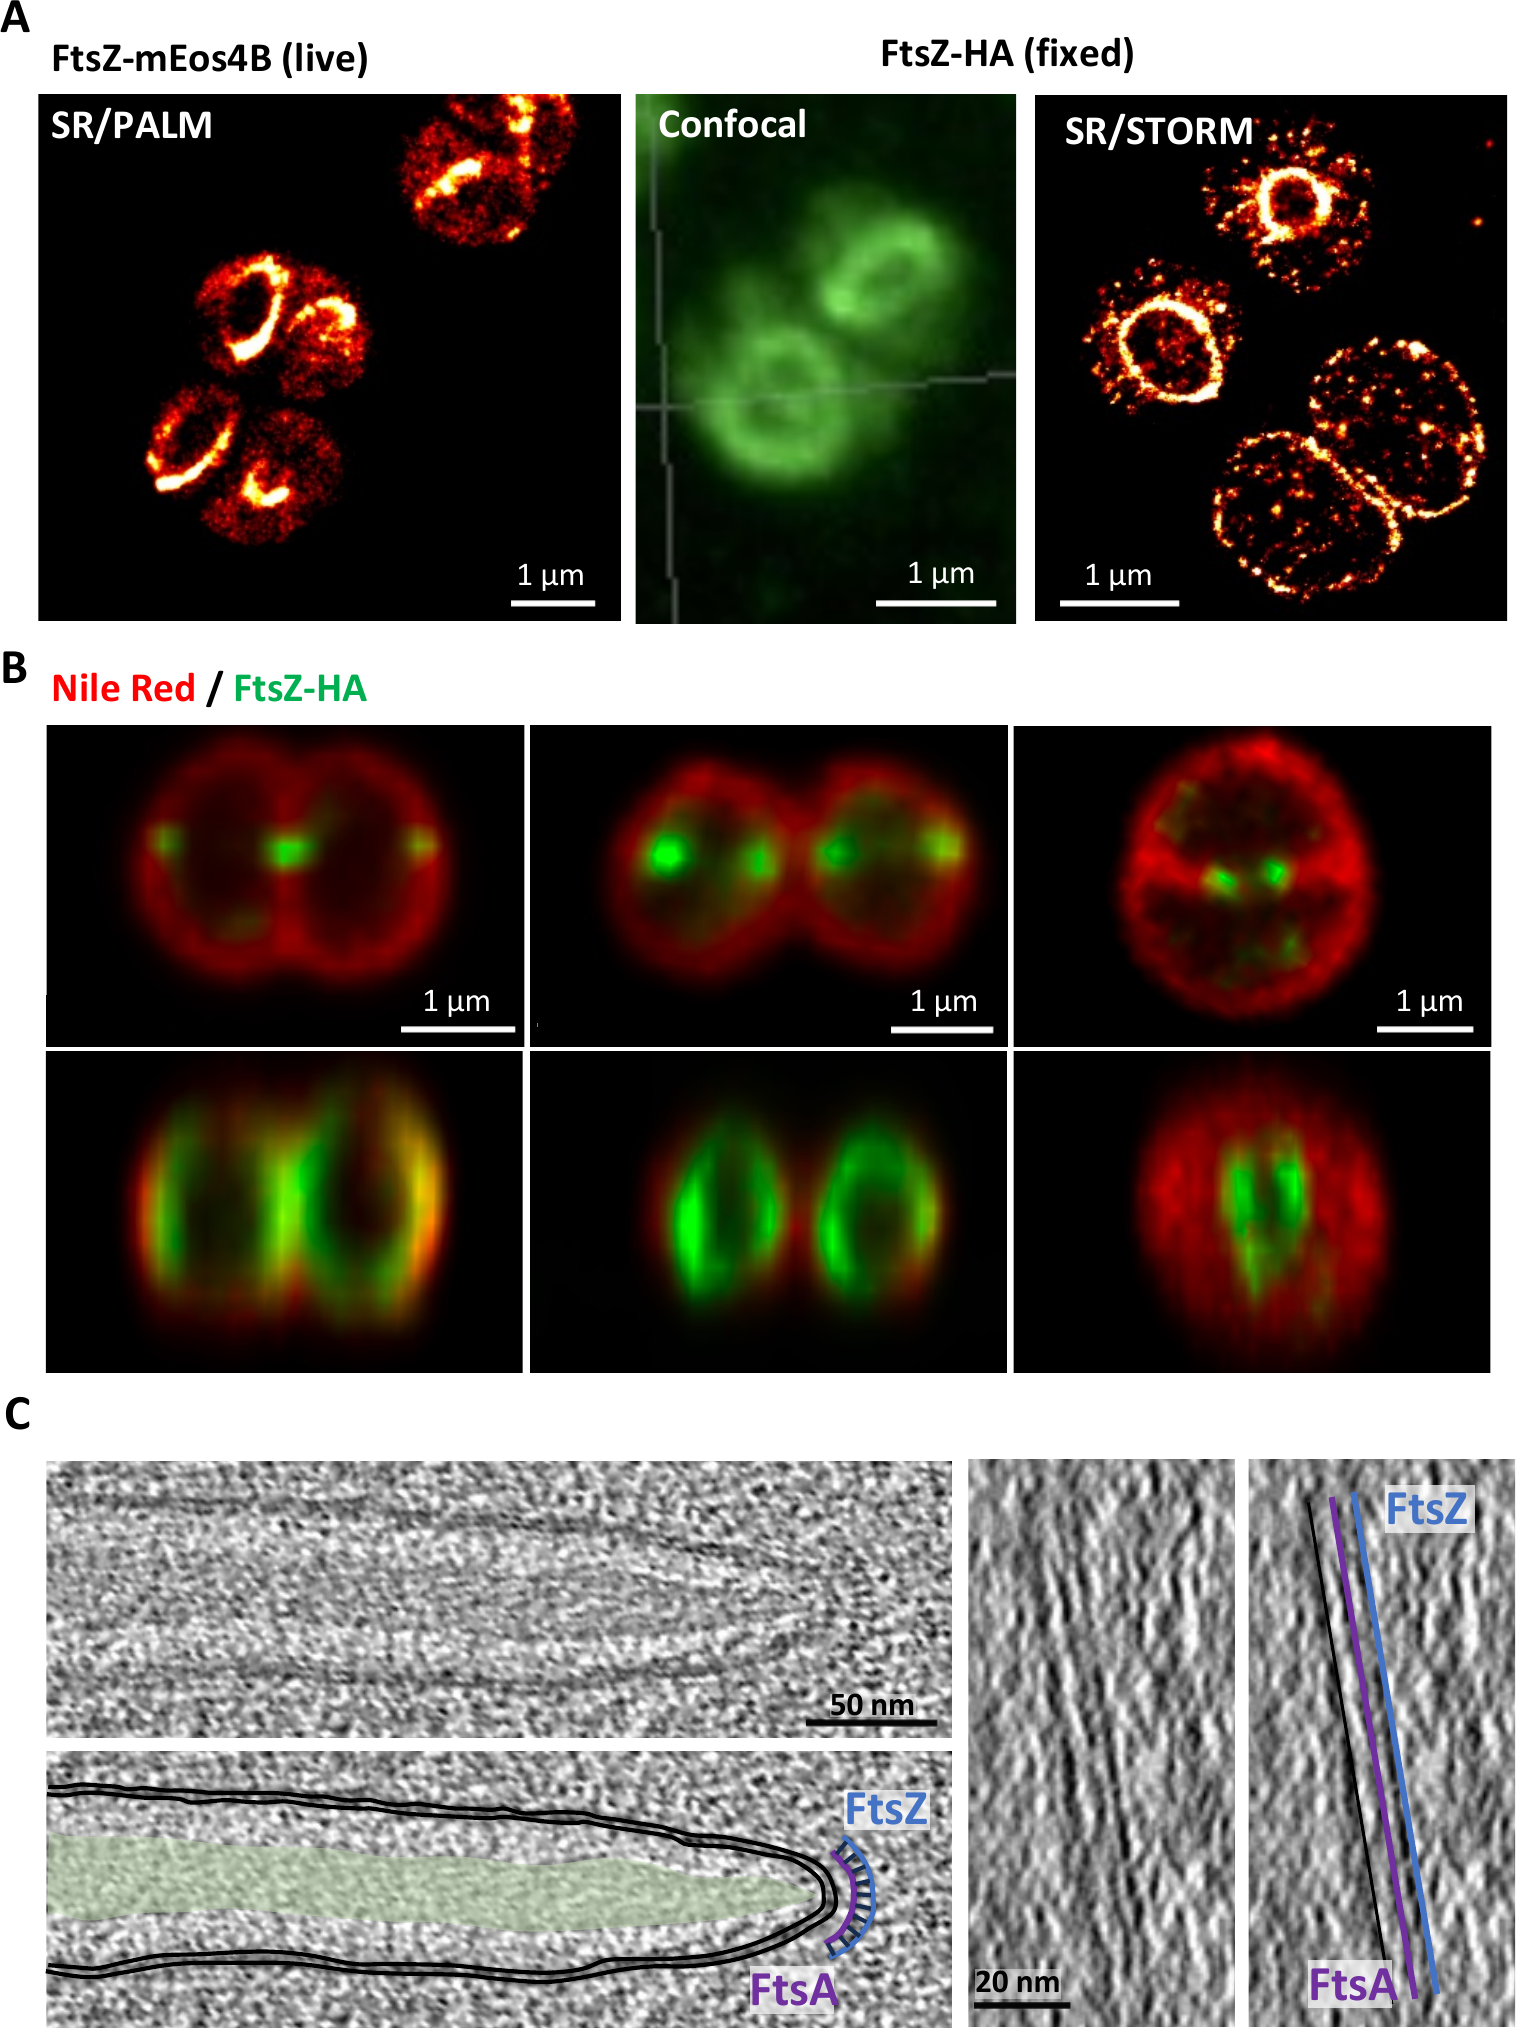
\includegraphics[width=\textwidth]{drad_paper/fig6.png}
    \caption{TODO}
    \label{drad_fig6}
\end{figure}

Examination of the tomograms revealed the presence of a double-arched structure situated at \sim\qty{15}{nm} from the septal tip, which likely corresponds to FtsZ (outer arch) and its cellular partner the membrane-bound FtsA~\cite{sextonSuperresolutionConfocalCryoCLEM2022} (inner arch; \autoref{drad_fig6}C).
These structures were again observed at all stages of the septation process as in our fluorescence microscopy data, and when looking at the z-projection, they were found to form long straight filaments characteristic of FtsZ.
Interestingly, FtsZ was not detected when septa were extended with membrane structures, suggesting that FtsZ only assembles at septal tips containing PG in close proximity to the membrane.
However, FtsZ was sometimes seen either above or below these membrane extensions, forming a discontinuous filament, which may explain the incomplete ring structures observed by fluorescence microscopy (\autoref{drad_fig6}A-B).

\FloatBarrier

\section{Discussion}

TODO: Brief summary of results.

\textit{D. radiodurans} is a spherical diderm bacterium that is known to possess a unique cell envelope including an outer S-layer, which has been the object of numerous studies over the past decades~\cite{vonkugelgenMultidomainConnectorLinks2022,workMorphologyChemistryCell1968,rothfussInvolvementSlayerProteins2006,vonkugelgenInterdigitatedImmunoglobulinArrays2023,farciSDBCActiveQuenching2023,farciStructuredOrganizationDeinococcus2022,farciCryoEMStructureSlayer2022,farciStructuralAnalysisArchitecture2021,baumeisterThreedimensionalStructureRegular1986,baumeisterStructureCellEnvelope1981}.
Bacteria from the \textit{Deinococcus-Thermus} phylum, such as \textit{D. radiodurans}, exhibit features of both Gram positive and Gram negative bacteria.
\textit{D. radiodurans} is indeed lacking lipopolysaccharides typically found in Gram negative bacteria, possesses a thick PG layer (\qty{35}{nm}-\qty{55}{nm}) characteristic of Gram positive bacteria and yet its cell envelope is composed of two membrane bilayers characteristic of Gram negative bacteria~\cite{guptaOriginDidermGramnegative2011}.
The exact composition and structure of this unusual cell wall has been the object of much controversy in the recent years, notably regarding the outer layers linking the PG to the outermost S-layer hexameric lattice structure.
Our cryoET analysis of the outer cell wall composition fully supports the model proposed by Bharat and colleagues, in which the whole cell wall is \sim\qty{100}{nm} in thickness and composed of two membranes in between which can be found a thin periplasmic space and two thicker layers, the PG and SlpA layers~\cite{vonkugelgenMultidomainConnectorLinks2022}.
The S-layer is then located \sim\qty{18}{nm} above the outer membrane~\cite{vonkugelgenInterdigitatedImmunoglobulinArrays2023}.
The SlpA layer takes its name from the major protein constituent of this layer, the SlpA protein, a trimeric porin-like protein that is embedded in the outer membrane and stretches across the SlpA layer via a long coiled-coil region to connect to the PG layer~\cite{vonkugelgenMultidomainConnectorLinks2022}.
The predicted length of this assembly (\sim\qty{28}{nm}-\qty{29}{nm}) is in good agreement with our estimated thickness of the SlpA layer (\qty{35}{nm}).
Interestingly, we observe a distinctive white line between the PG and SlpA layers that may correspond to the sites at which the N-terminal SLH domain of SlpA attaches to the PG layer.

\subsection{Cell wall structure and composition} -- discuss earlier studies by Piano et al and Bharat et al.

\subsection{Progressive splitting of cells by action of hydrolases} -- tight coupling with synthesis of outer layers.

\subsection{Septation process} -- Closing door mechanism \& progressive filling of membranes to form rigid septa.
Distinct PG synthesis machinery in septa and in outer cell wall.
Outer cell wall machinery may be largely located at junction of septum and outer cell wall whereas septum-specific machinery is located at tip of growing septa.

Mesosomes: Similar structures were reported in early studies of \textit{D. radiodurans}~\cite{thornleyFineStructureMicrococcus1965,sleytrStudyFreezeetchingFine1973} and other model bacteria~\cite{suganumaStudiesFineStructure1966,pontefractMesosomesEscherichiaColi1969} in the 1960's, but were later considered as artefacts of chemical fixation procedures used for electron microscopy sample preparation~\cite{ryterContributionNewCryomethods1988,dubochetElectronMicroscopyFrozenhydrated1983,liedtkeHowAdvancesCryoelectron2022}.

\subsection{FtsZ} -- present at all stages, linked to PG layer, coordinated PG synthesis and septal growth and ensuring opposite septa meet at mid-cell.
More work needed to decipher exact mechanisms and regulatory factors.

\section{Materials \& Methods}

\subsection{Bacterial cultures}

\textit{D. radiodurans} (DR) strains used in this study are listed in Table S1.
All strains were derivatives of the wild-type strain R1 ATCC 13939 (DR\textsuperscript{WT}).
The genetically engineered strain of \textit{D. radiodurans} expressing FtsZ fused to mEos4B (DR-\textit{FtsZ-mEos4B}) was obtained by the tripartite ligation method as described recently~\cite{vauclareStressinducedNucleoidRemodeling2024}.
A synthetic gene encoding mEos4B was amplified together with the kanamycin resistance cassette by PCR as were the regions (\sim500bp) flanking the insertion site (3' end of \textit{ftsZ} gene and region immediately downstream of the \textit{ftsZ} gene) using oligonucleotides listed in Table S2.
After restriction digestion the three fragments were ligated together and transformed into \textit{D. radiodurans}.
Transformants were selected on TGY agar plates containing \qty{6}{\mu{}g/ml} kanamycin, leading to allelic replacement on one genome copy.
Because \textit{D. radiodurans} is multigenomic, the transformant colonies were streaked three times successively on selective medium to ensure that all copies of the genome had incorporated the foreign DNA.
This was then confirmed by PCR analysis and DNA sequencing.
\textit{D. radiodurans} cells were grown aerobically at \ang{30}C in a shaking incubator (160 rpm) in Tryptone-Glucose-Yeast extract 2x (TGY2X) medium supplemented with the appropriate antibiotics.
Typically for microscopy experiments, \textit{D. radiodurans} cells were pre-grown the day before and then diluted for an overnight growth until reaching exponential (OD\textsubscript{650} \sim0.3-0.5) the next morning.
Optical density measurements were made on a Clariostar (BMG Labtech) plate reader.

\subsection{Cell labelling for confocal and single-molecule localisation (SMLM) microscopy}

Membranes of exponential phase DR bacteria were stained by addition of Nile Red (30 \mu{}M for confocal microscopy and 30-100 nM for SMLM) to the growth medium of cells (1 ml) for 10 min at room temperature.
The cells were then harvested by centrifugation and resuspended in 200 \mu{}l TGY2X for confocal microscopy or instead washed 3 times in DPBS (3x 1 ml) and resuspended in 200 \mu{}l DPBS for SMLM.
10 \mu{}l of this cell suspension was then placed on the bottom of a glass dish and cells were allowed to sediment for 2 min.
Excess liquid was gently removed using a pipette and after 2 minutes of air-drying, 10 \mu{}l 1.5\% (w/v) low melting agarose (LMA; Bio-Rad) equilibrated at \ang{37}C was poured over the cells.
The LMA was prepared in TGY2X medium for timelapse confocal imaging and in DPBS for PAINT imaging of Nile Red labelled bacteria.
For PG labelling, 1.5 ml of exponential phase DR cultures were centrifuged at 3000xg and resuspended in 200 \mu{}l TGY2X medium to which 50 \mu{}l 10 mM azido-D-Alanine (zDA) was added.
Pulse labelling was typically performed for 10 min at \ang{30}C, before washing the cells two times with cold DPBS to stop cell growth.
Cells were then resuspended in 48 \mu{}l 30 \mu{}M DBCO-AF488 or \textbf{DBCO-AF647} (dSTORM) diluted in DPBS and incubated on ice for 45 min to allow the DBCO-AF488/AF647 to enter the bacteria and react by click chemistry with the incorporated zDA.
When ready to be imaged, labelled cells were washed two times with DPBS and resuspended in 100 \mu{}l DPBS.
3-5 \mu{}l of cell suspension was then deposited on a 1.5\% LMA pad prepared using a gene frame positioned on a cover glass.
For PALM imaging of FtsZ-mEos4B, DR-\textit{FtsZ-mEos4B} cells were grown to exponential phase, washed twice with DPBS and deposited directly on a 1.5\% LMA pad prepared in DPBS using a gene frame positioned on a cover glass.
For immunolabelling of HA-tagged FtsZ, DR-\textit{FtsZ-HA} (strain GY15705) bacteria were grown to exponential phase.
0.5 ml culture was fixed at \ang{4}C overnight by addition of 3.7\% formaldehyde directly to the culture medium.
The cells were then washed twice in DPBS and resuspended in 100 \mu{}l DPBS.
Cells were permeabilized by treatment with 4 mg/ml lysozyme at \ang{37}C for 30 min followed by the addition of 0.1\% Triton X-100 for 5 min at \ang{25}C.
Cells were then washed twice with DPBS and incubated with a mouse anti-HA antibody (1:400 dilution in PBS-tween0.05\% supplemented with 2\% BSA) for 1h at \ang{37}C.
After several washes with PBS-tween0.05\%, cells were incubated with anti-mouse secondary antibody coupled to either Alexa fluor 488 (for confocal) or Alexa Fluor 647 (for dSTORM) for 1h at \ang{37}C.
After a final washing step, the bacteria were deposited on a 1.5\% LMA pad prepared in DPBS using a gene frame positioned on a cover glass.
For dSTORM experiments, the LMA was prepared in glucose buffer (62.5 mM Tris-HCl pH 8.0, 12.5\% glucose, 12.5 mM NaCl) and contained 0.1M MEA and 1x GLOX (\textbf{??}).
For confocal microscopy, the LMA was prepared as above in TGY2X.

\subsection{Confocal data acquisition and processing}

Spinning-disk confocal microscopy was performed using an Olympus IX81 inverted microscope equipped with a Yokogawa CSU-X1 confocal head.
The excitation laser beam (Ilas2 laser bench, GATACA systems) was focused to the back focal plane of a 100X 1.49-numerical-aperture (NA) oil immersion apochromatic objective.
Series of Z-planes were acquired every \qty{100}{nm} using a PRIOR N400 piezo stage.
Fluorescence excitation was performed at \qty{488}{nm} for DBCO-AF488 and \qty{561}{nm} for Nile Red.
Fluorescence emission was collected with an Andor iXon Ultra EMCCD camera through a quad-band Semrock\texttrademark Di01-T405/488/568/647 dichroic mirror and single-band emission filters adapted to each fluorophore used: \qty{520}{nm} for DBCO-AF488 (FF02-520/28 Semrock\texttrademark), and \qty{600}{nm} for Nile Red (ET600/50m Chroma\texttrademark).
Data acquisition was performed using Metamorph 7.10 (Molecular devices).

\subsection{Image correction for timelapse videos Kymographs.}

\subsection{SMLM (PAINT/dSTORM) data acquisition and processing}

PAINT and dSTORM data were acquired on a SAFE 360 (Abbelight) SMLM set up.
Data was acquired at \ang{27}C under continuous illumination with 400 W/cm² \qty{561}{nm} light or \qty{640}{nm} light and a frame time of 8-\qty{10}{ms}.
\textbf{40,000 -- 60,000} frames were acquired per dataset.

\subsection{Cryo-FIB milling}

\subsection{Cryo Electron tomography}

\subsection{CryoET data processing}

\newpage

\section{Supplemental Figures}

\begin{figure}[ht]
    \centering
    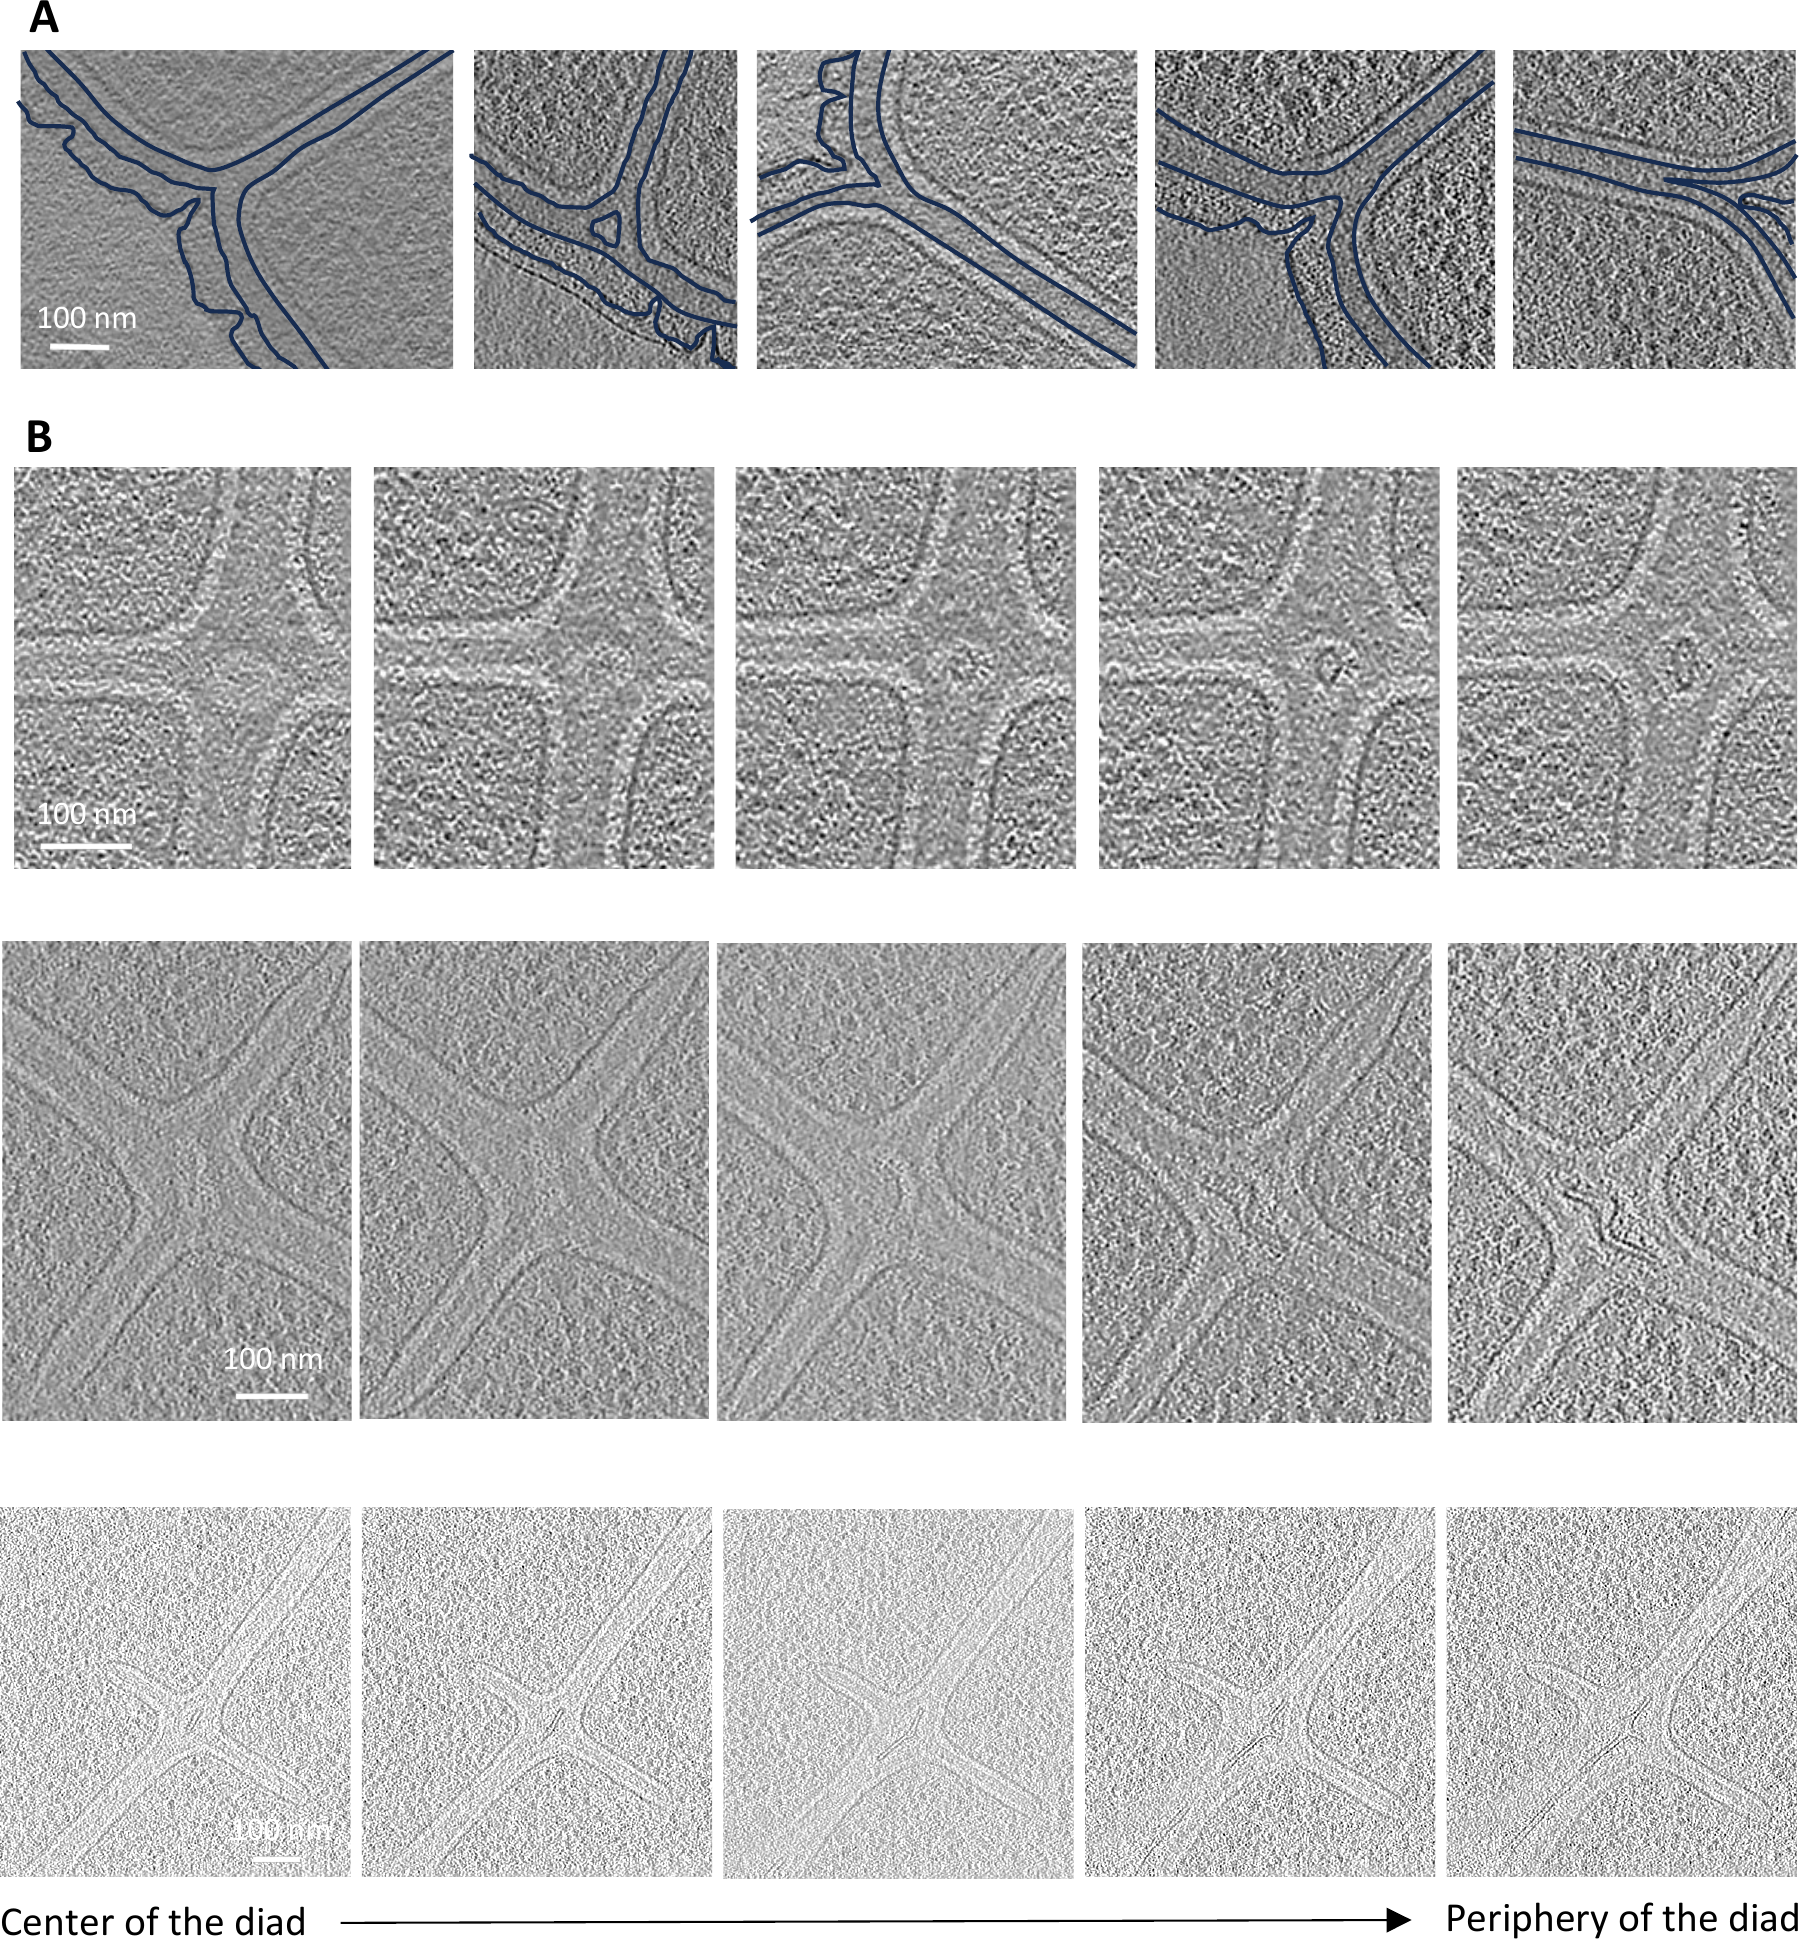
\includegraphics[width=\textwidth]{drad_paper/sfig1.png}
    \caption{TODO}
    \label{drad_sfig1}
\end{figure}

\begin{figure}[ht]
    \centering
    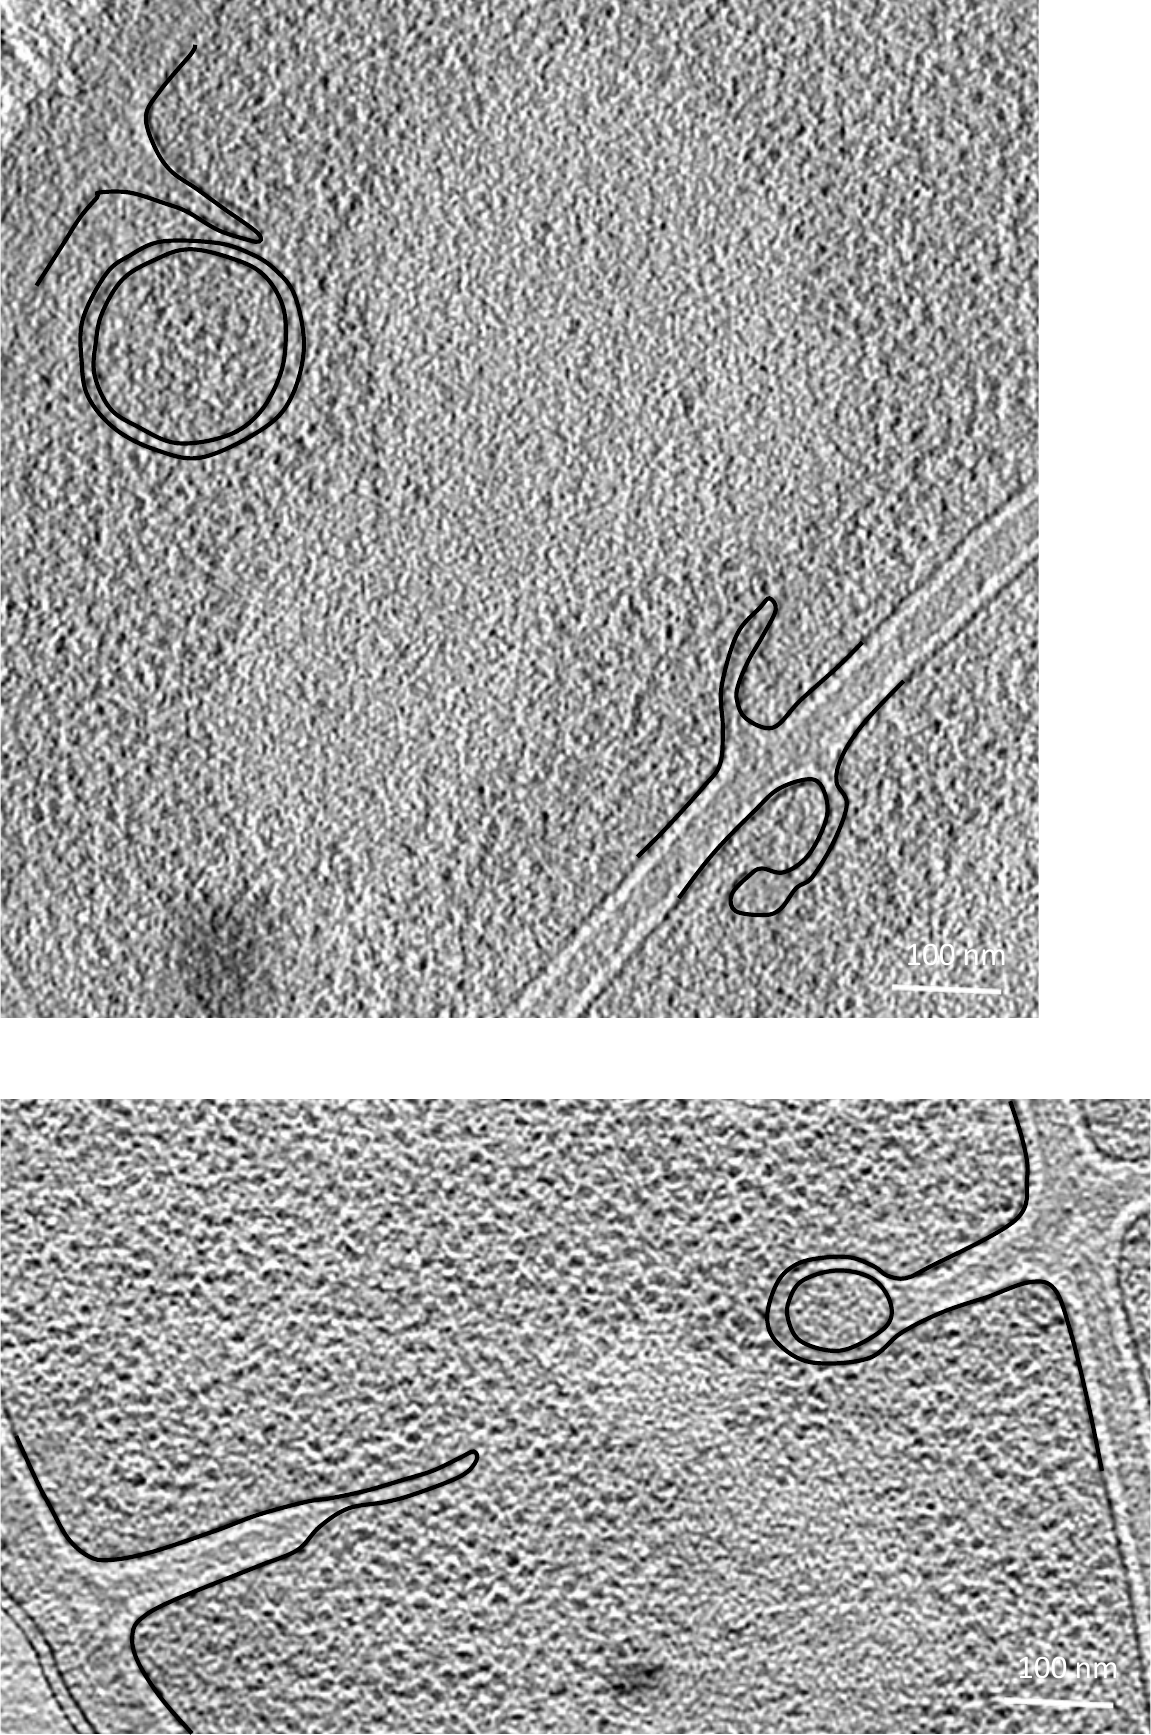
\includegraphics[width=.8\textwidth]{drad_paper/sfig2.png}
    \caption{TODO}
    \label{drad_sfig2}
\end{figure}

\begin{figure}[ht]
    \centering
    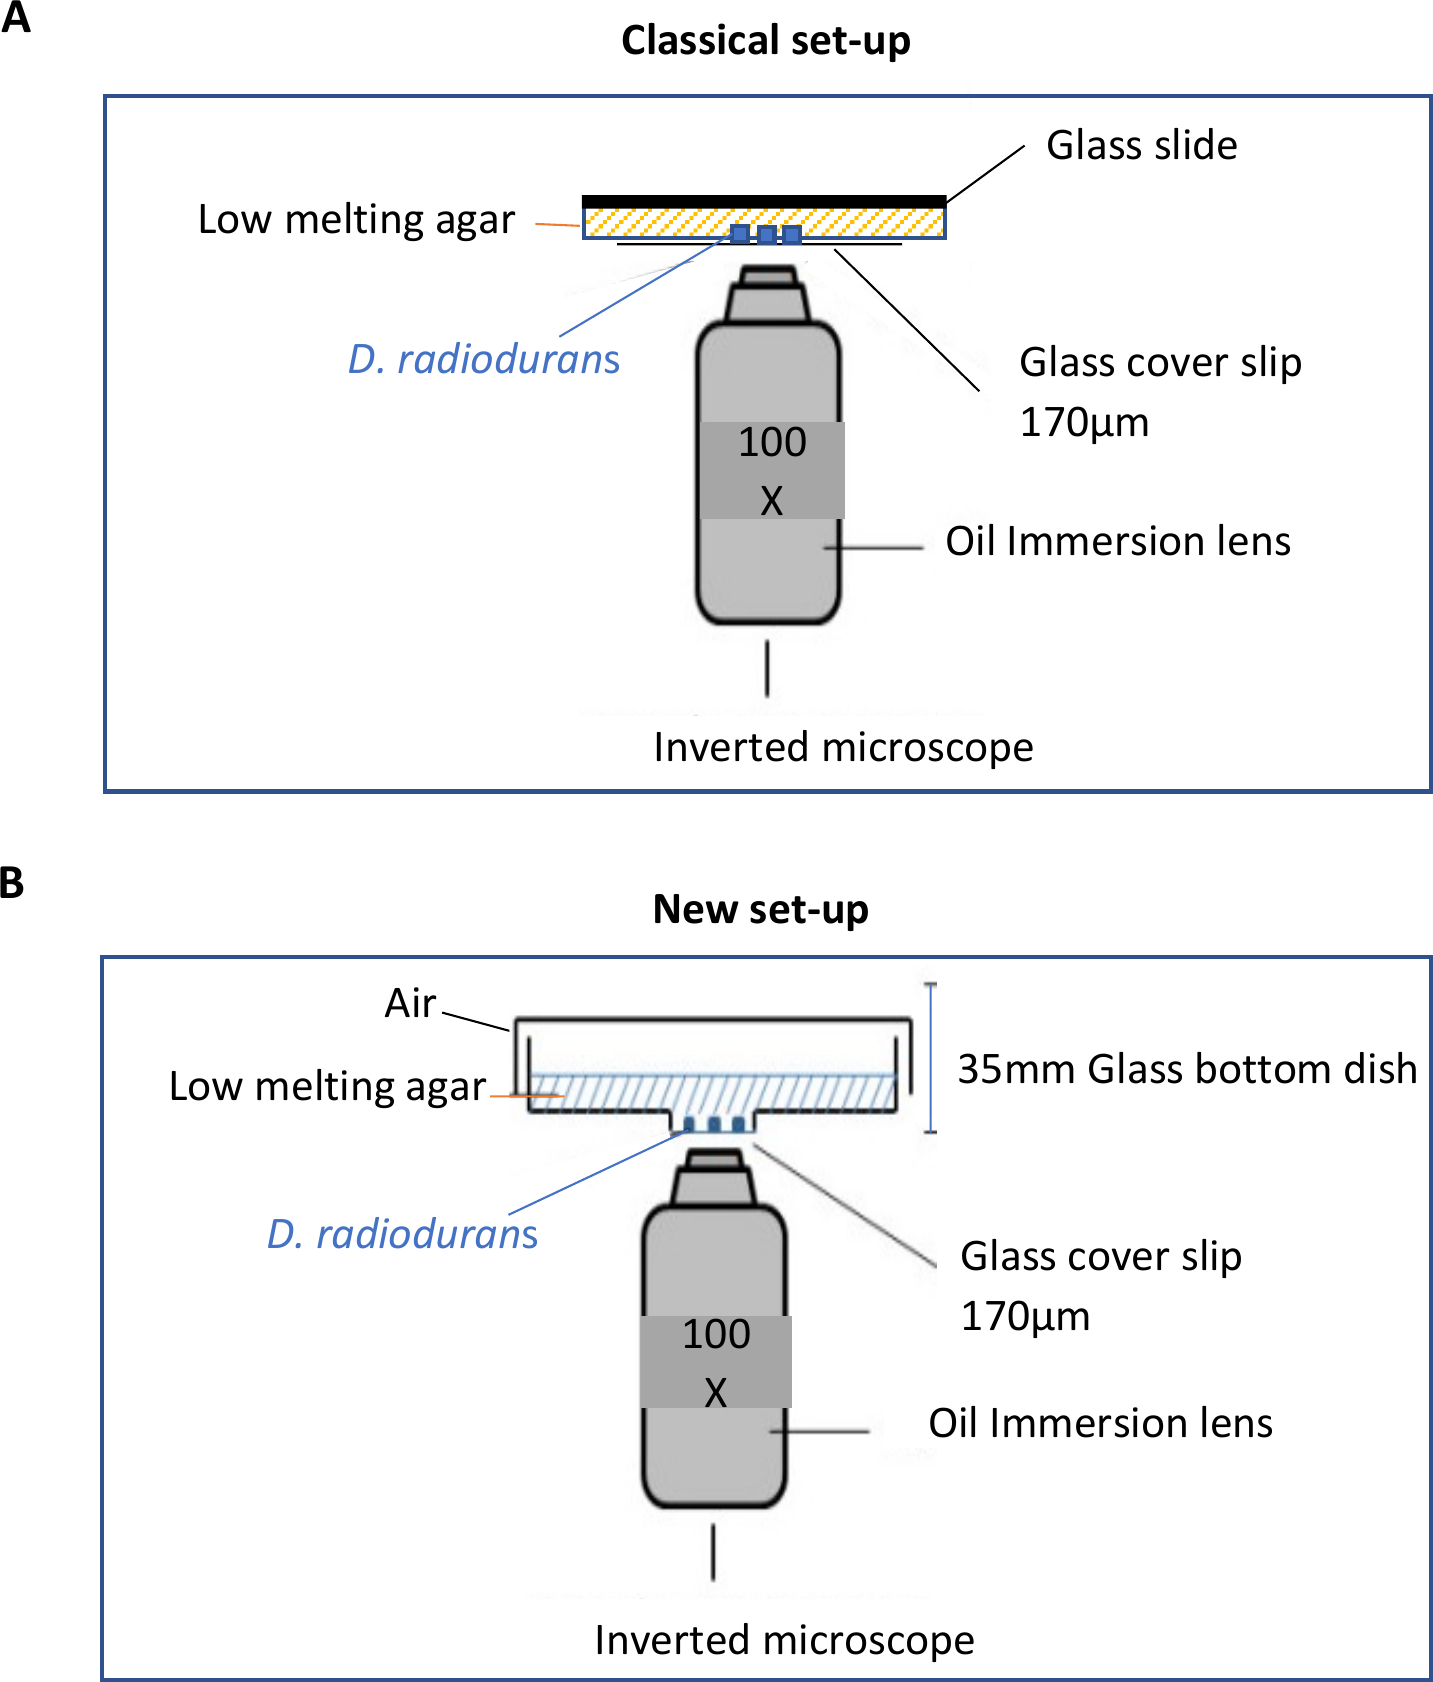
\includegraphics[width=\textwidth]{drad_paper/sfig3.png}
    \caption{TODO}
    \label{drad_sfig3}
\end{figure}

\begin{figure}[ht]
    \centering
    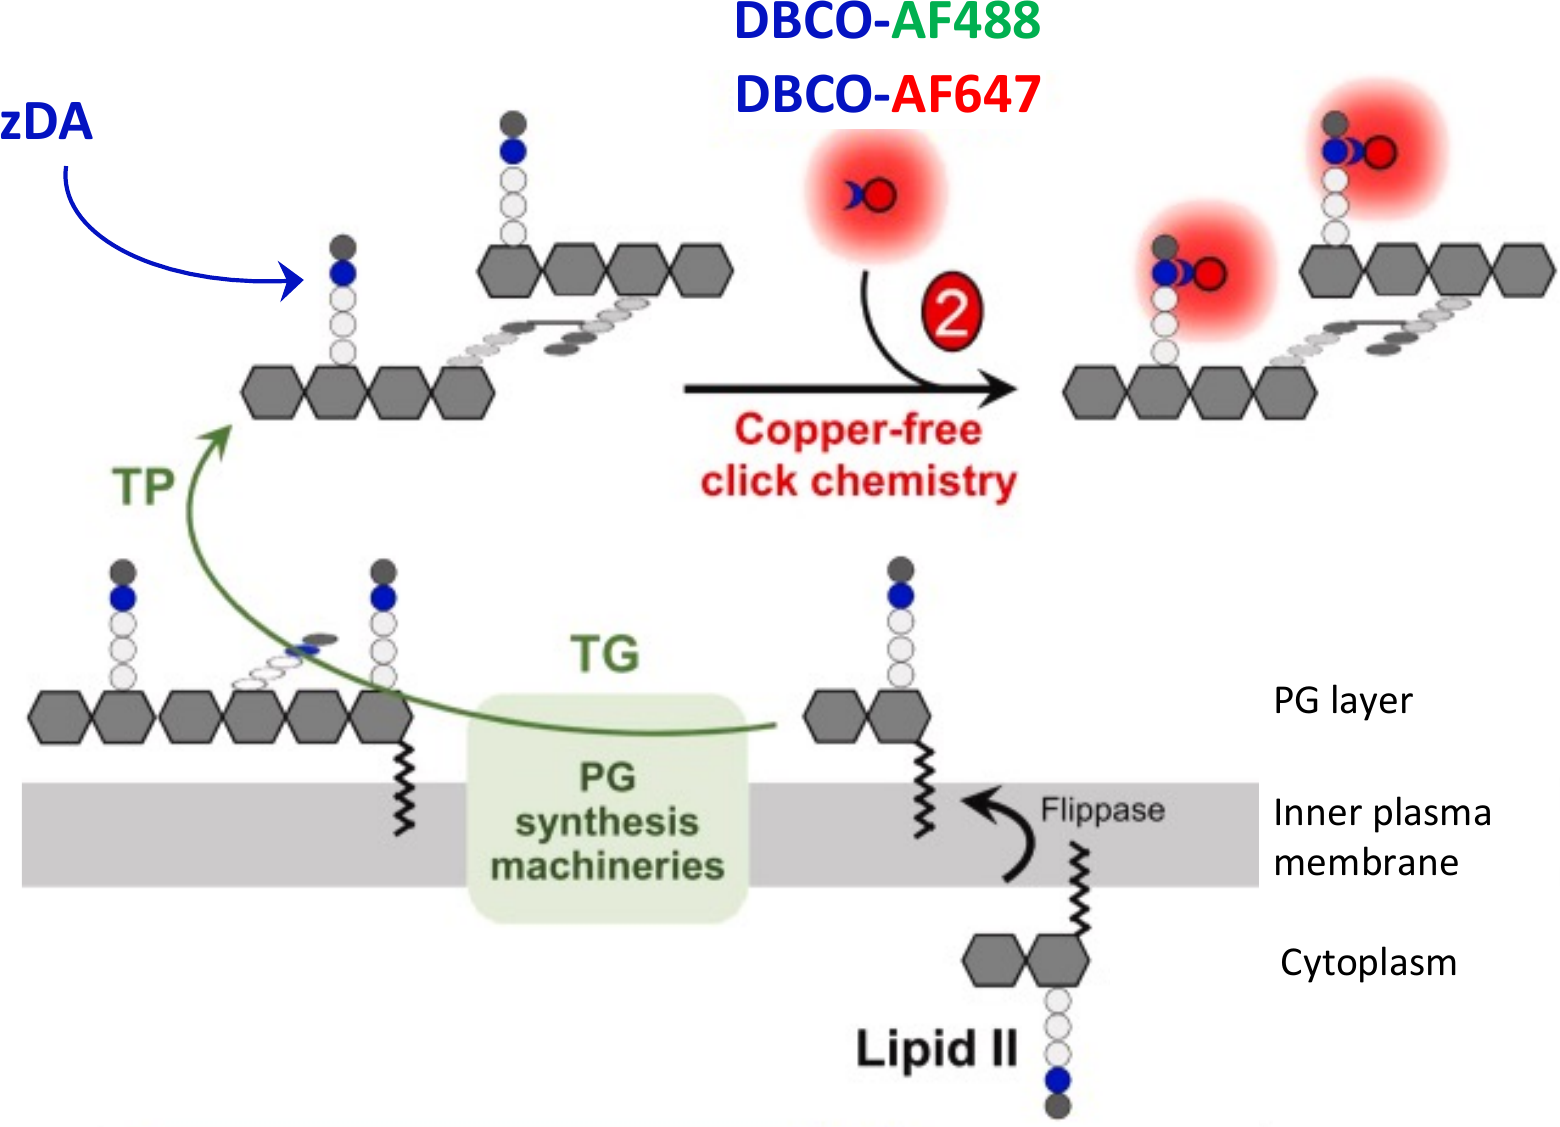
\includegraphics[width=\textwidth]{drad_paper/sfig4.png}
    \caption{TODO}
    \label{drad_sfig4}
\end{figure}

\begin{figure}[ht]
    \centering
    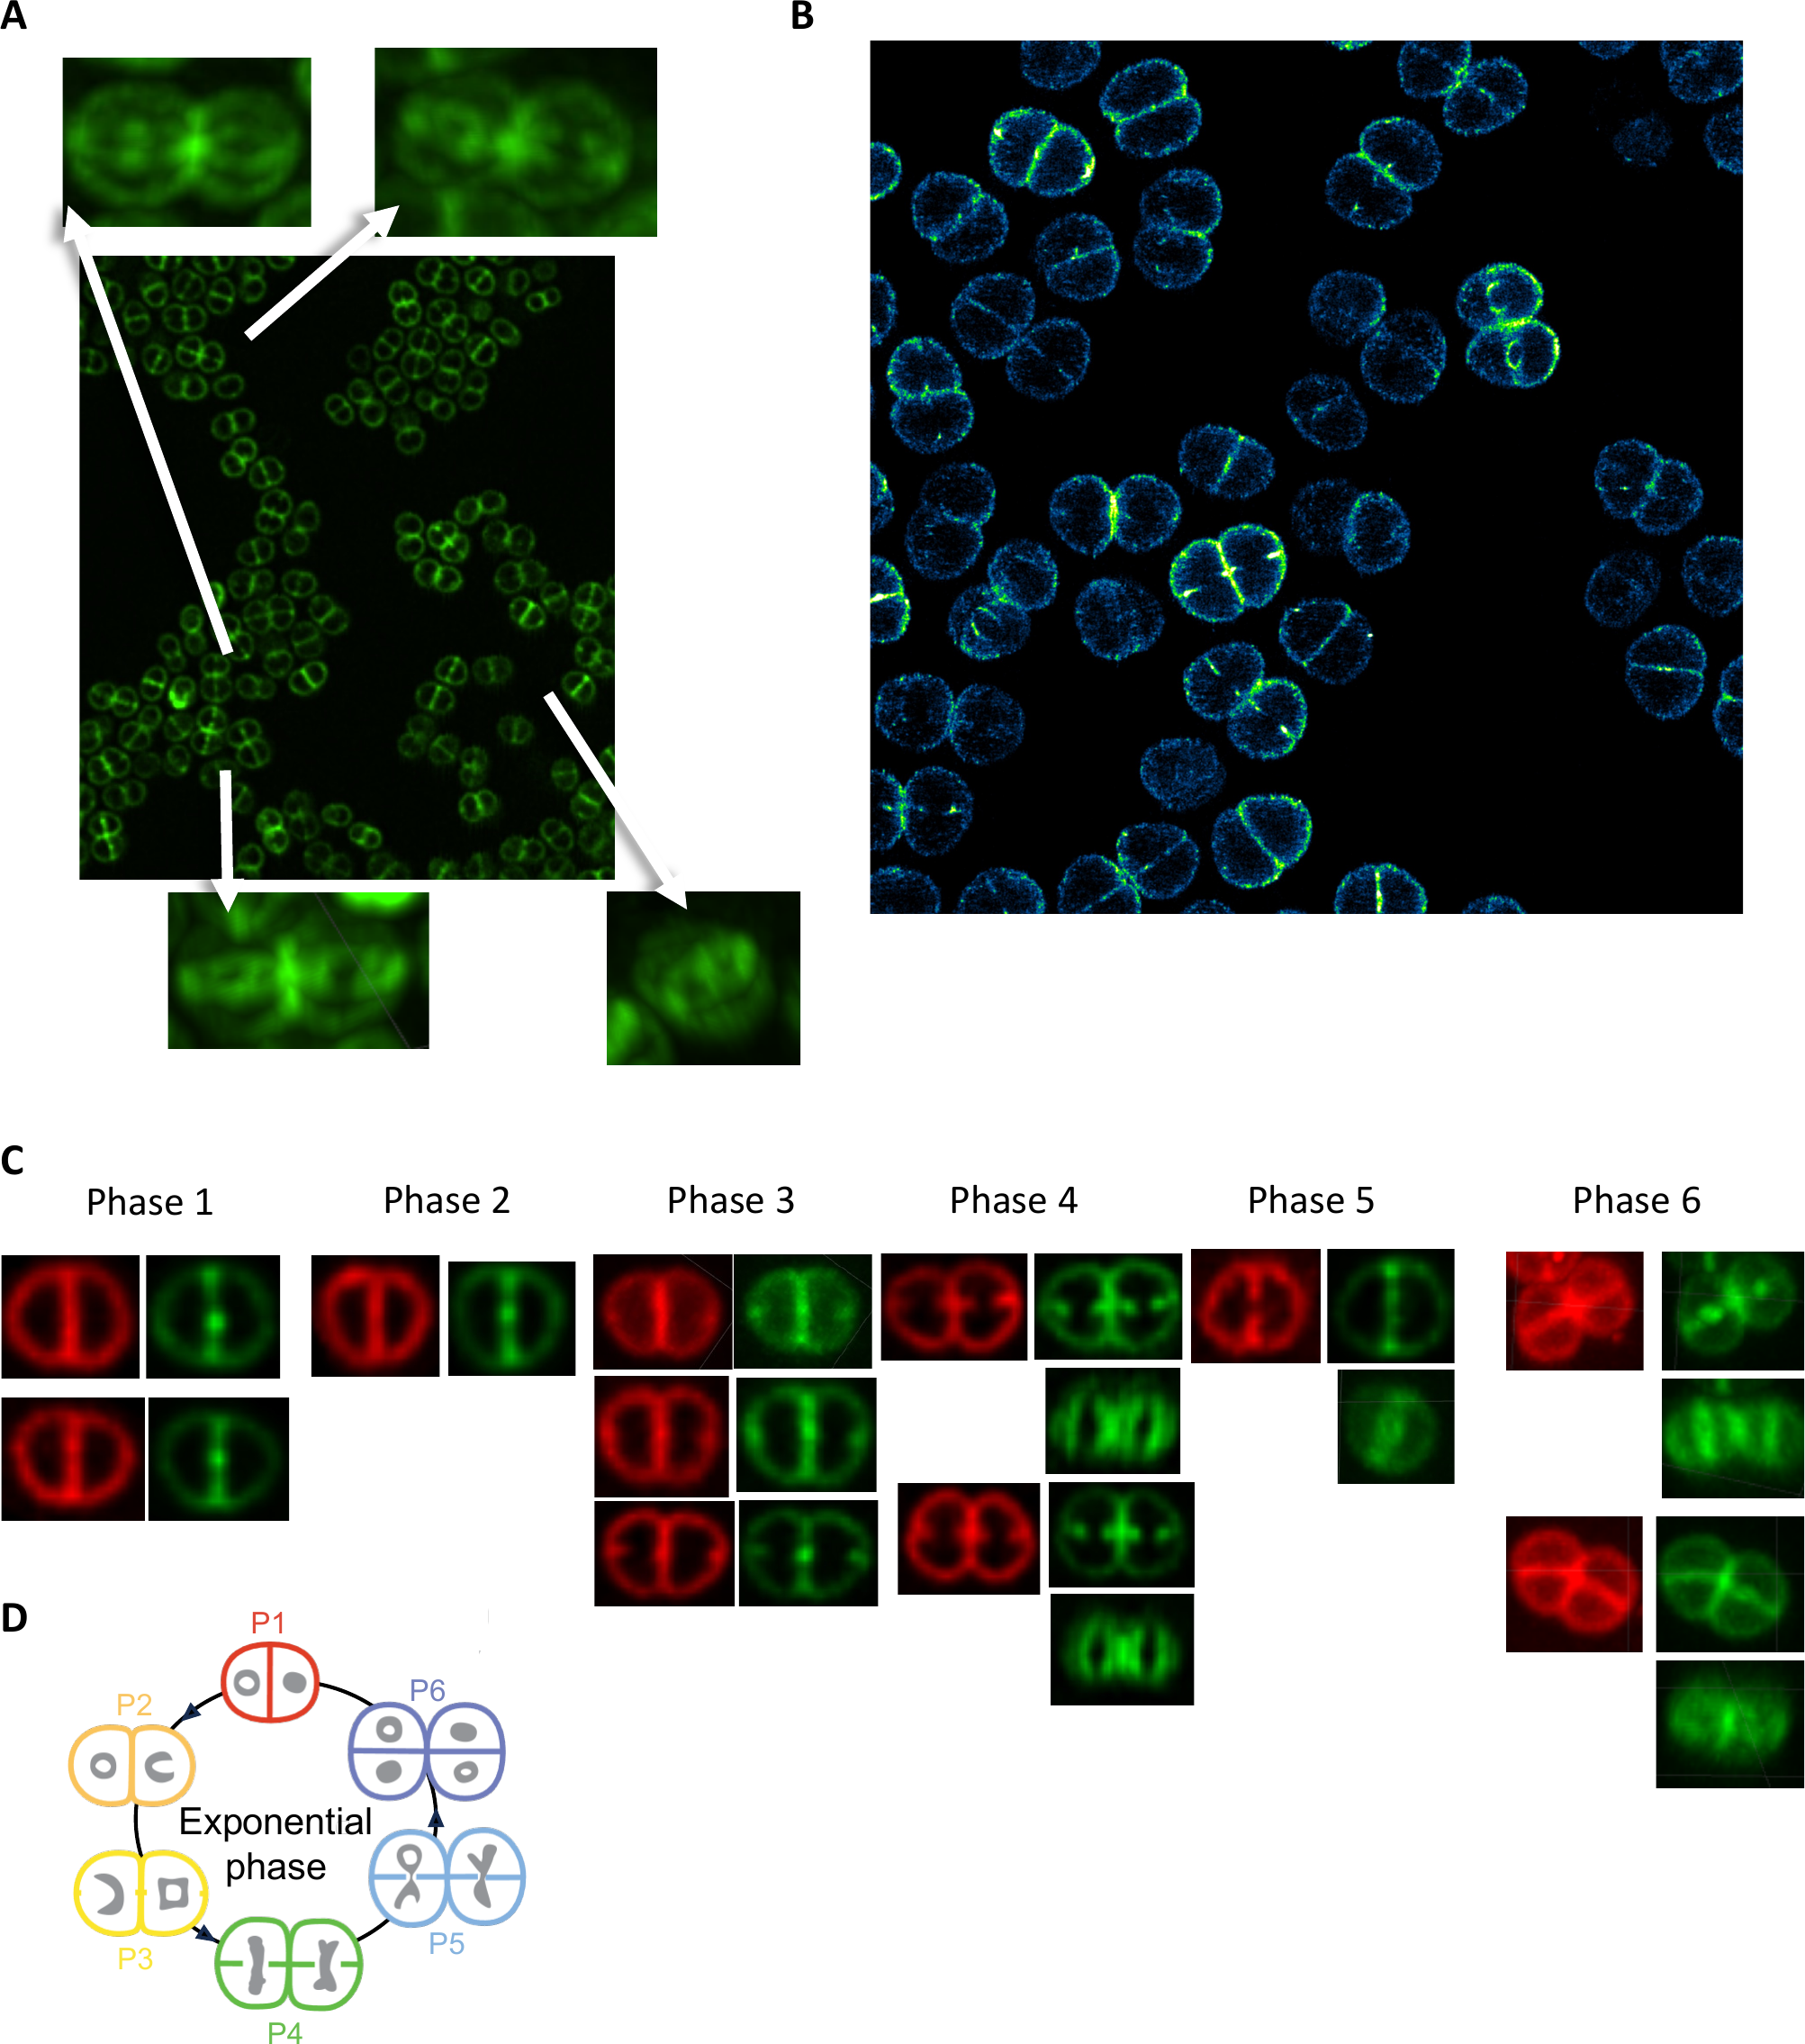
\includegraphics[width=\textwidth]{drad_paper/sfig5.png}
    \caption{TODO}
    \label{drad_sfig5}
\end{figure}

\begin{figure}[ht]
    \centering
    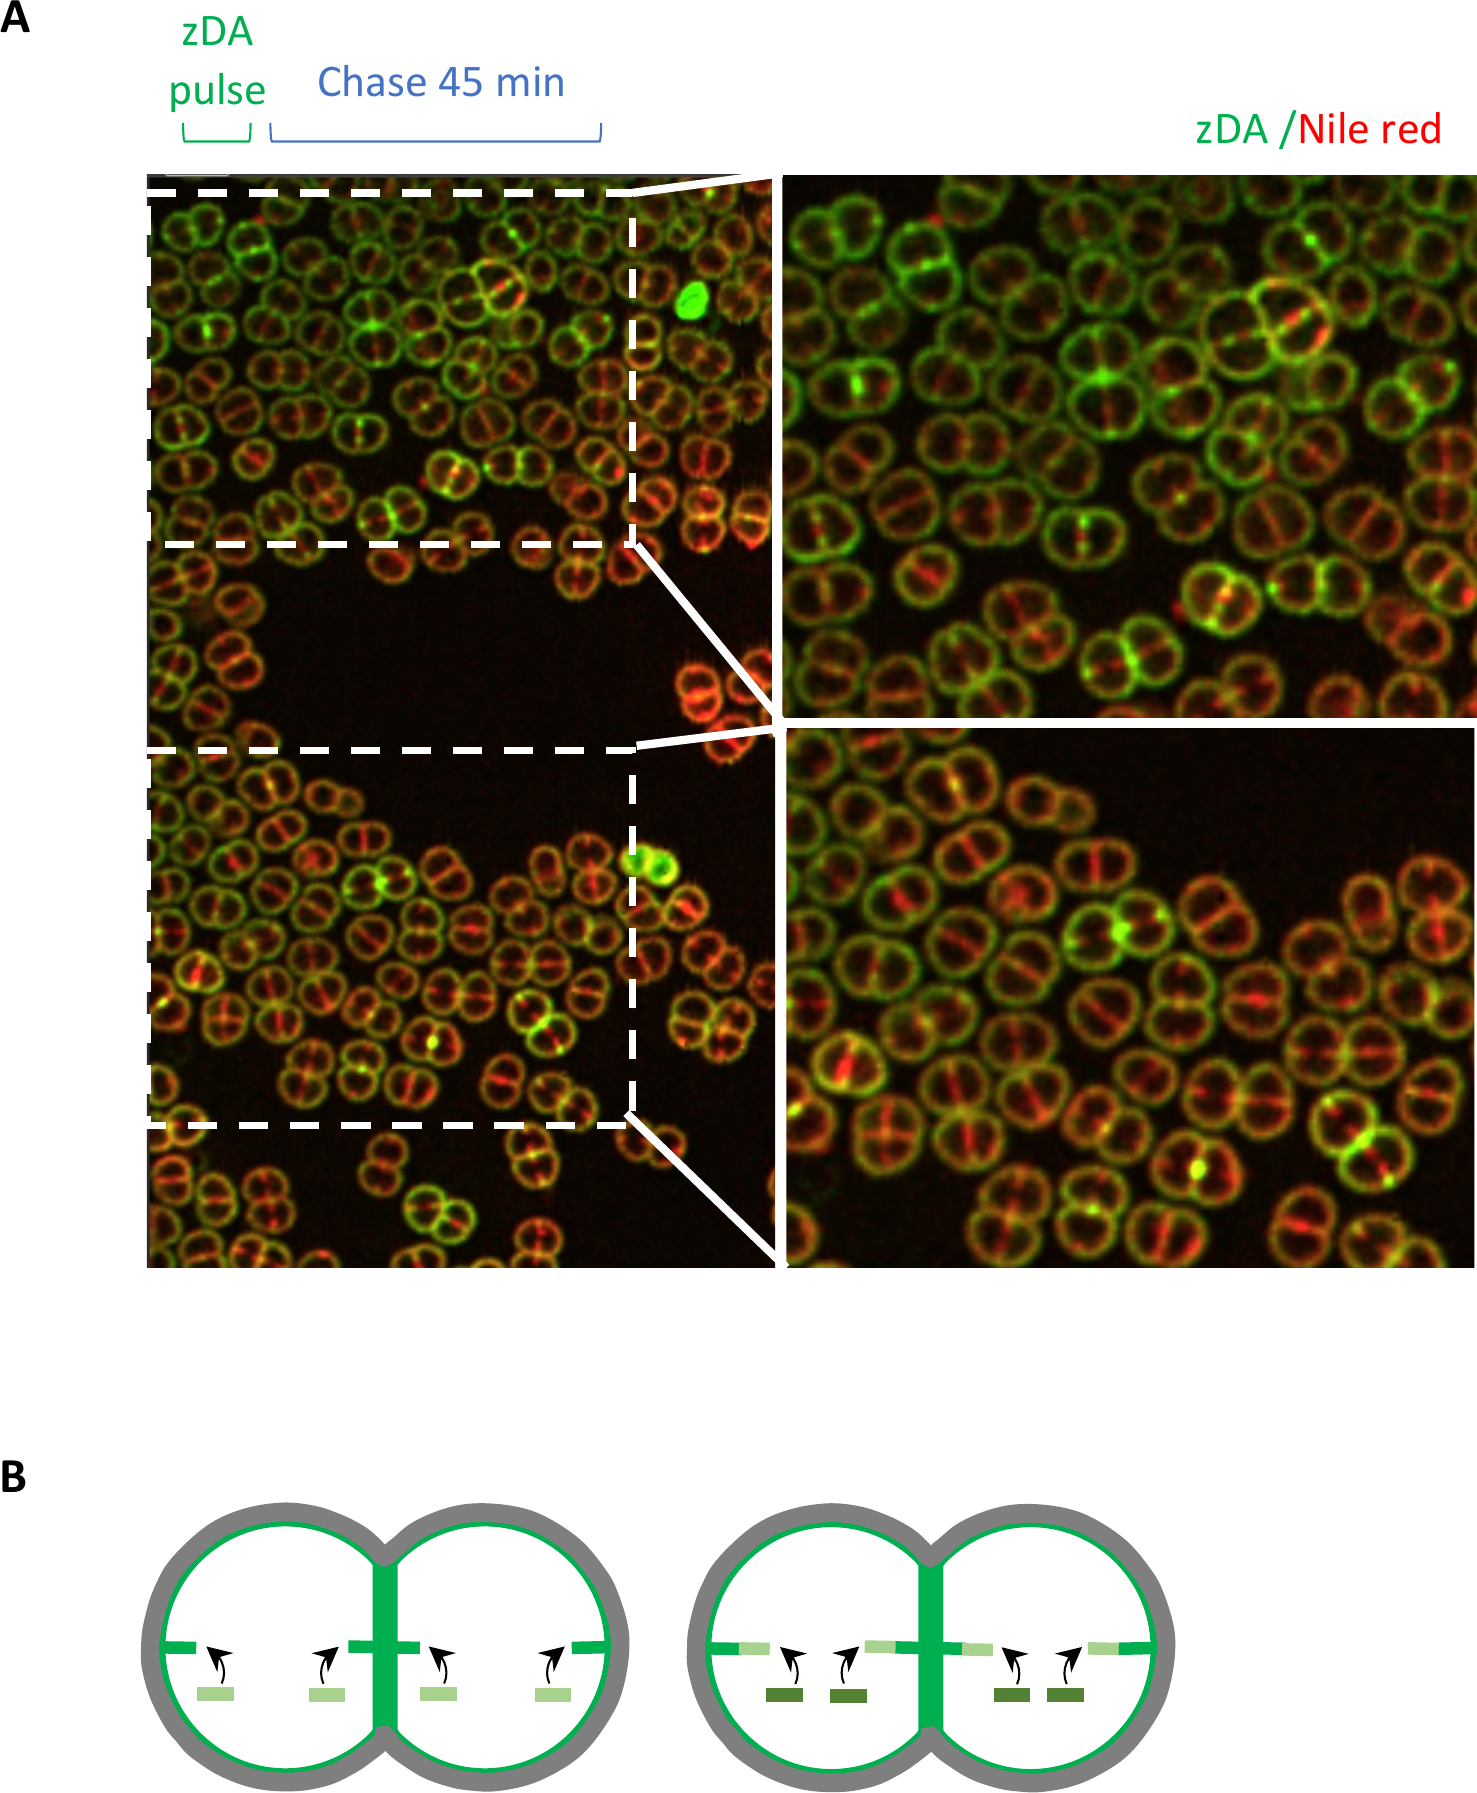
\includegraphics[width=\textwidth]{drad_paper/sfig6.png}
    \caption{TODO}
    \label{drad_sfig6}
\end{figure}

\begin{figure}[ht]
    \centering
    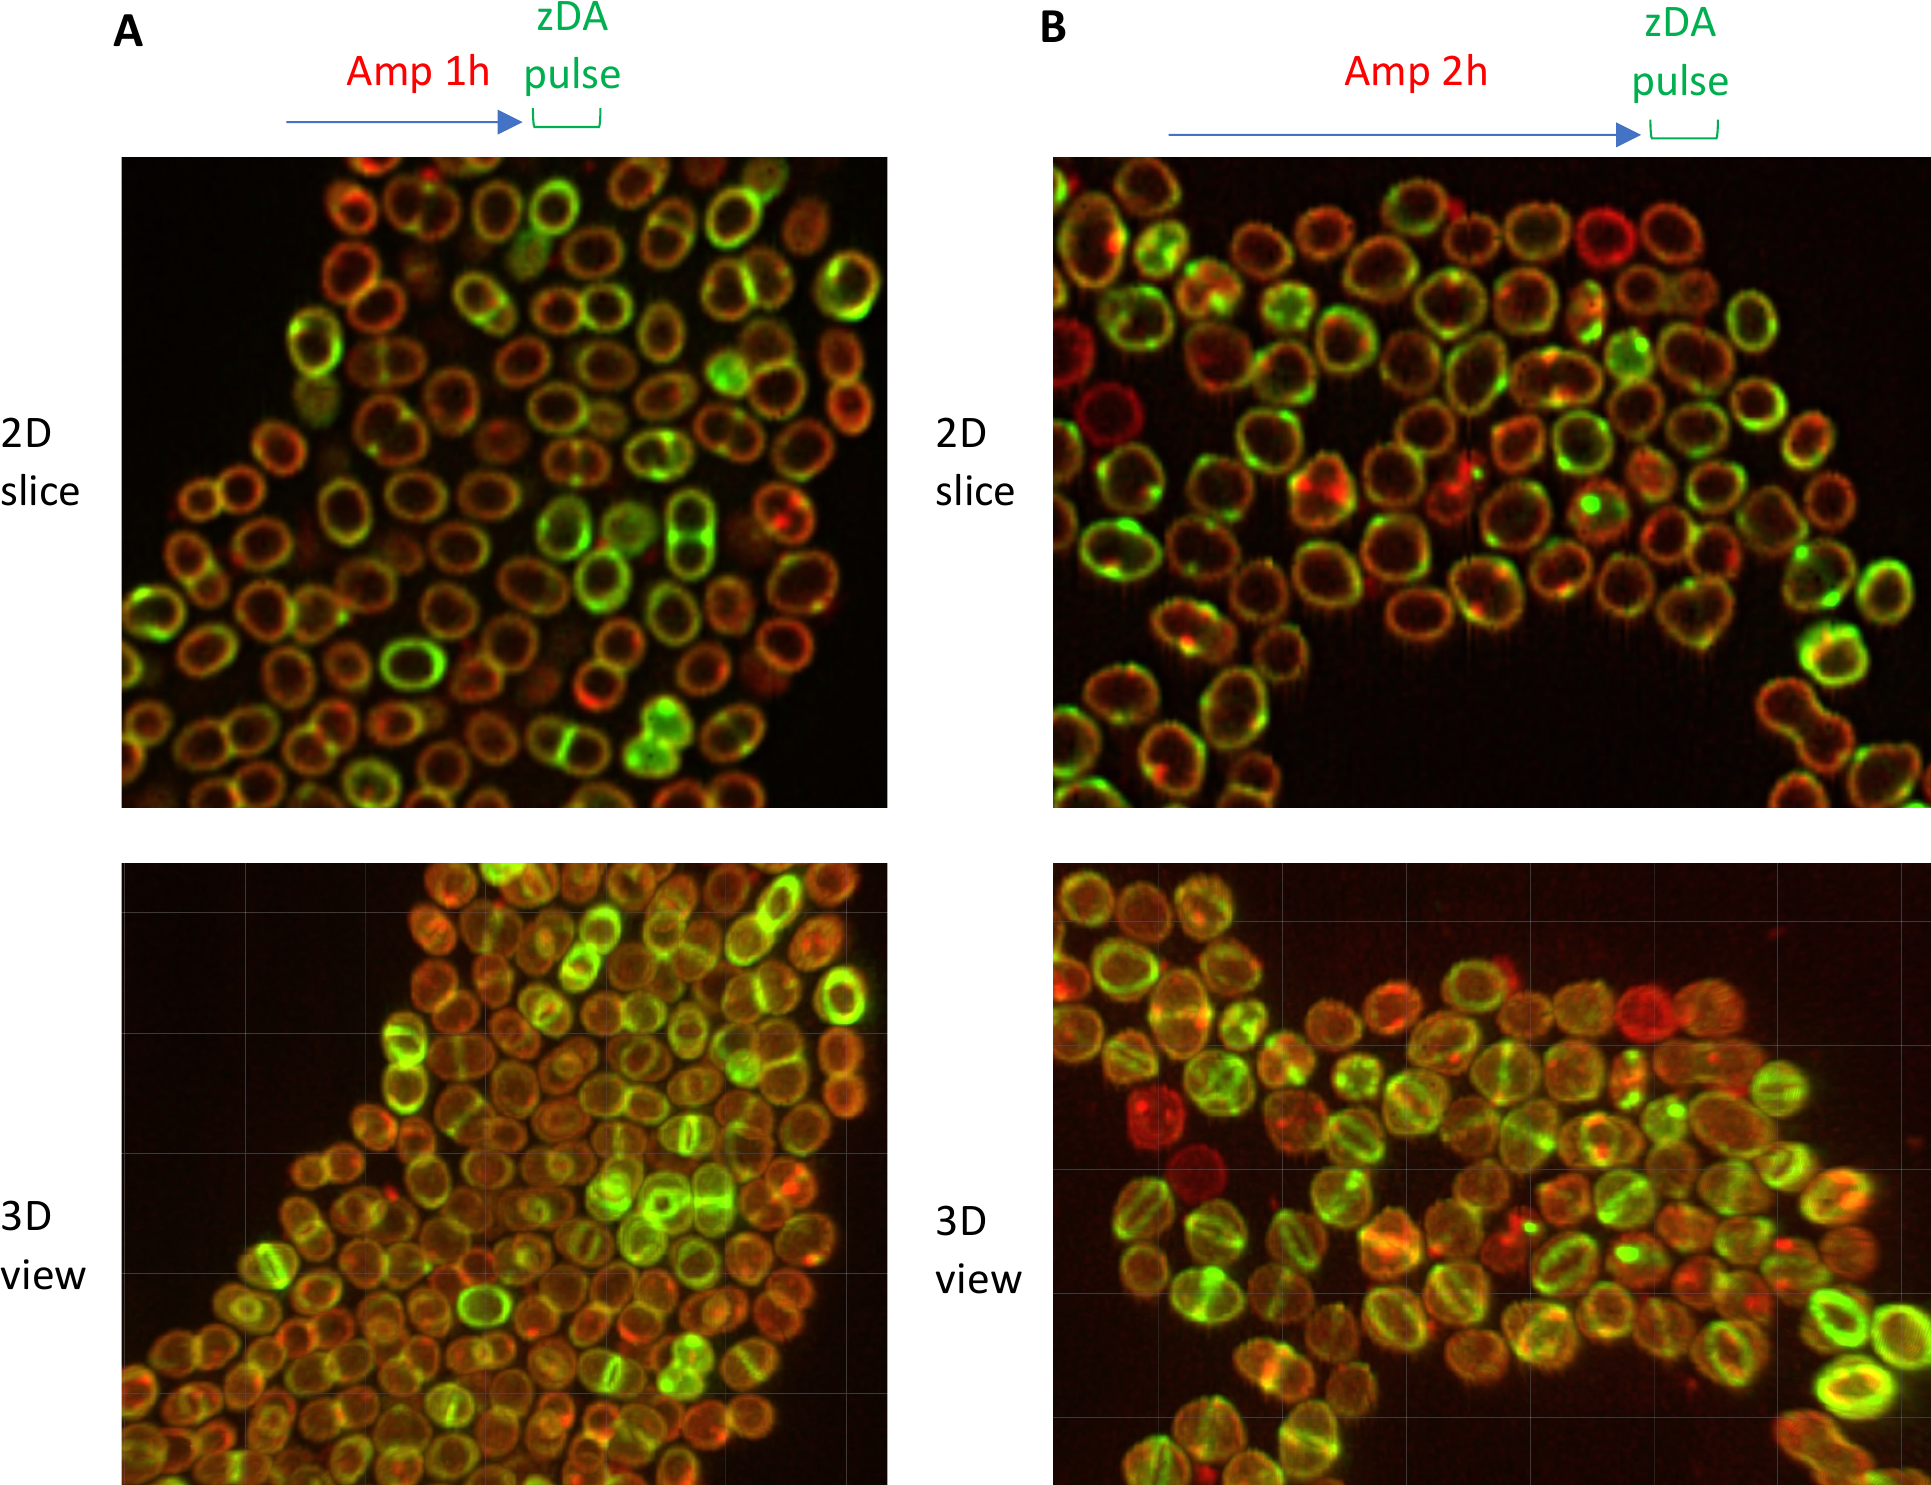
\includegraphics[width=\textwidth]{drad_paper/sfig7.png}
    \caption{TODO}
    \label{drad_sfig7}
\end{figure}

\FloatBarrier


\section{Addendum}

TODO: Some info on ftsz and so on.

        \chapter{FtsZ: function and structure}\label{ftsz}

To better understand the role of FtsZ in the septation of \textit{D. radiodurans}, we investigated its structure and superstructure using both single particle cryo-EM and \textit{in situ} cryo-ET.
This work is ongoing and not yet consolidated into a manuscript for publication.
Sample preparation and screening was performed by my supervisors Irina Gutsche and Joanna Timmins, while data collections were done partly by Irina, and partly commissioned to external facilities.
Data processing on the single particle and tomography data, and software tool development were performed by me, and progressively handed off to Harald Bernhard, a postdoc in the MICA group.

\localtableofcontents

\section{State of the art}

FtsZ is an extremely well conserved prokaryotic tubulin homologue, known to form ring-like structures (the Z-ring) at the septation site in most bacteria.
It polymerizes in a GTP-dependent fashion to form filaments and bundles, anchoring to the membrane via its partner FtsA, and interacting with several other partners in the cytokinesis and peptidoglycan (PG) synthesis machinery~\cite{barrowsFtsZDynamicsBacterial2021,mcquillenInsightsStructureFunction2020}.

Based on crystal structures, filaments have been shown to form through head-to-tail stacking of monomers CITE.
However, there is no structural information regarding the flexible C-terminal region, which is responsible for regulating its activity and interaction with its cellular partners, including FtsA.
It's also unclear how multiple filaments may assemble to form bundles at the structural level and even less so in vivo.
Thus --- while its key role in cell division is undisputed --- the exact mechanism and function of FtsZ are still unclear.
There is currently no consensus model that fully explains the function and mode of action of FtsZ in the division process in bacteria, as the current evidence is inconclusive, sometimes presenting significant variations between species --- likely ascribable to different shapes or membrane compositions between bacteria~\cite{barrowsFtsZDynamicsBacterial2021,mcquillenInsightsStructureFunction2020}.

\begin{figure}[ht]
    \centering
    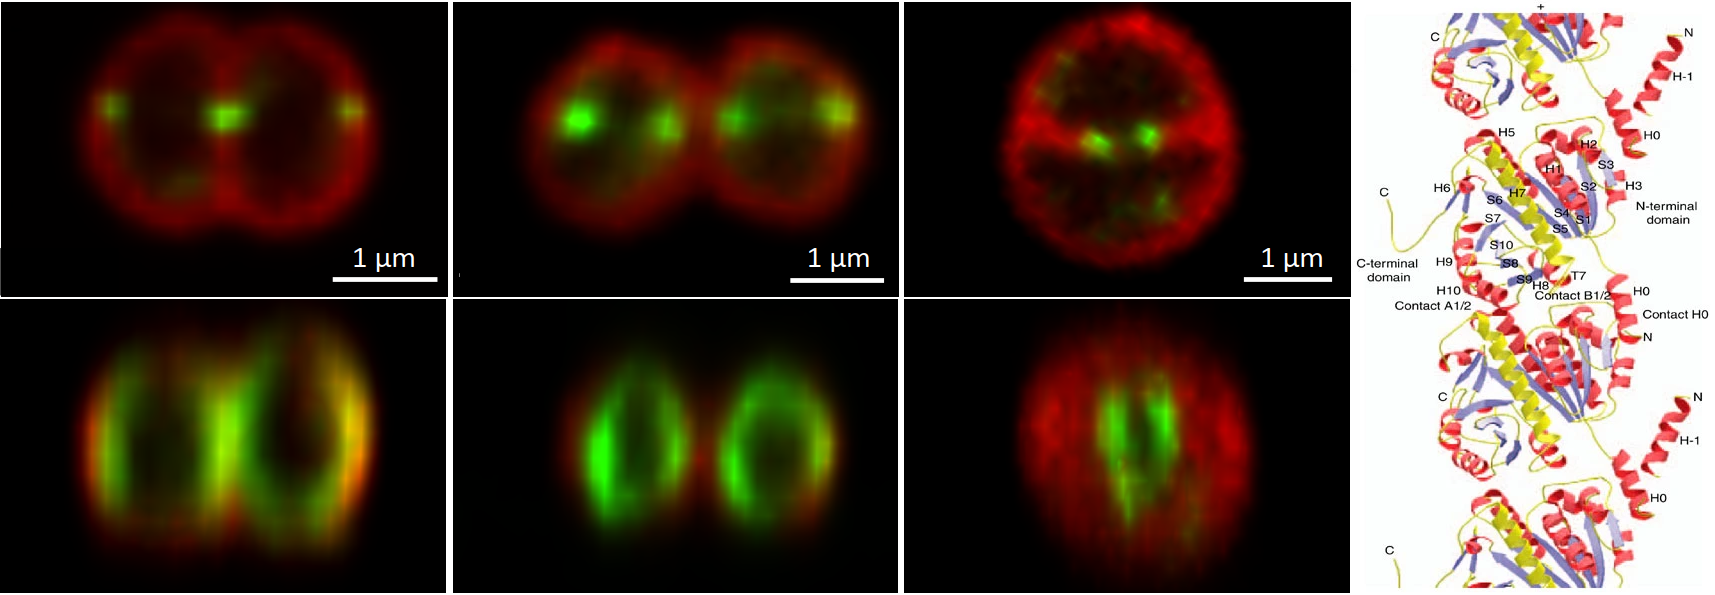
\includegraphics[width=\textwidth]{other/ftsz_ring.png}
    \titledcaption[FtsZ forms a ring \textit{in vivo} and filaments \textit{in vitro}]{During cell division, FtsZ is known to localize on a ring (termed Z-ring) corresponding to the tips of the septa (left, figure adapted from \autoref{drad_fig6}). Many structural studies were done on FtsZ, identifying the formation of protofilament via head-to-tail stacking (right, figure adapted from \citet{olivaStructuralInsightsFtsZ2004}.}
    \label{fig:ftsz_ring}
\end{figure}

Some studies have shown that FtsZ presents mechanical functions that may drive the septation process.
\textit{T. maritima} FtsZ+FtsA expressed in liposomes was shown to form coil-like structures, which can constrict the membrane via a "filament sliding" mechanism, creating a partial septum~\cite{szwedziakArchitectureRingFormed2014}.
In \textit{C. crescentus}, FtsZ may form short, loosely bundled filaments, which may drive constriction via an "iterative pinching" mechanism where repeated rounds of phosphorylation lightly bend the filament, thus slowly pinching the membrane~\cite{liStructureFtsZFilaments2007}.

Other publications investigated the recruitment and signalling role of FtsZ for downstream machinery such as PG synthesis.
FtsZ was shown to undergo plus-end polymerization and minus-end depolymerization, in a GTP-regulated process typical of cytoskeletal proteins called treadmilling~\cite{looseBacterialCellDivision2014}.
In \textit{B. subtilis}, this treadmilling is required to drive the movement along the septum of the PG synthesis centers~\cite{bisson-filhoTreadmillingFtsZFilaments2017}.
A "diffusion-and-capture" model was proposed, where the FtsZ ring performs a recruitment role by engaging in weak transient interactions with downstream machinery for PG synthesis~\cite{baranovaDiffusionCapturePermits2020}.
However, in \textit{S. aureus}, cytokinesis may actually occur in two separate steps: a slow, FtsZ-driven, treadmilling-dependent step which causes initial invagination, followed by a faster step where PG synthesis is the driving force for septation~\cite{monteiroPeptidoglycanSynthesisDrives2018}.

While FtsZ ring formation and PG synthesis are clearly linked, their precise interaction may differ between bacteria.
In \textit{E. coli}, GTP regulates FtsZ treadmilling, which in turn controls the movement of the synthesis machinery~\cite{yangGTPaseActivityCoupled2017}.
However, it does not appear to affect the rate of PG synthesis, as opposed to what happens in \textit{B. subtilis}, which suggest that the presence or absence of an outer membrane may change PG synthesis machinery regulation~\cite{yangGTPaseActivityCoupled2017}.
Indeed, in \textit{E. coli}, some additional proteins may help with a timely invagination of the outer membrane, although they are not needed for septation to occur~\cite{gerdingTransenvelopeTolPal2007}.
This is intriguing for \textit{D. radiodurans} which, despite staining gram-positive, presents an outer membrane.

The disordered C-terminal domain of FtsZ was found to be necessary both for the anchorage to the membrane via FtsA, and to regulate oligomerization as well as bundling with neighboring filaments~\cite{barrowsFtsZDynamicsBacterial2021}.

Collectively, the literature hints that FtsZ treadmilling is likely not the only factor that controls the dynamics of FtsZ and the Z-ring, and that variations across species may be explained by different divergent mechanisms, or some other underlying behavior not yet discovered~\cite{barrowsFtsZDynamicsBacterial2021}.

\section{Structural study by SPA}

We began our investigation of the structure of DrFtsZ filaments by doing SPA on \textit{in vitro} samples prepared with purified monomeric FtsZ from \textit{D. radiodurans}.
Since successful polymerization is highly sensitive to FtsZ concentration, temperature, concentration of GTP (or other nucleotide), and elongation time, my supervisors tested a variety of conditions, using both negative stain EM and cryo-EM for screening.
The selected preparation(\fullref{ftsz_methods}) resulted in FtsZ filaments long enough to allow filament picking and helical reconstruction, while avoiding an excess of filament bundles which make picking and refinement more difficult (\autoref{fig:ftsz_micrographs}).

\begin{figure}[ht]
    \centering
    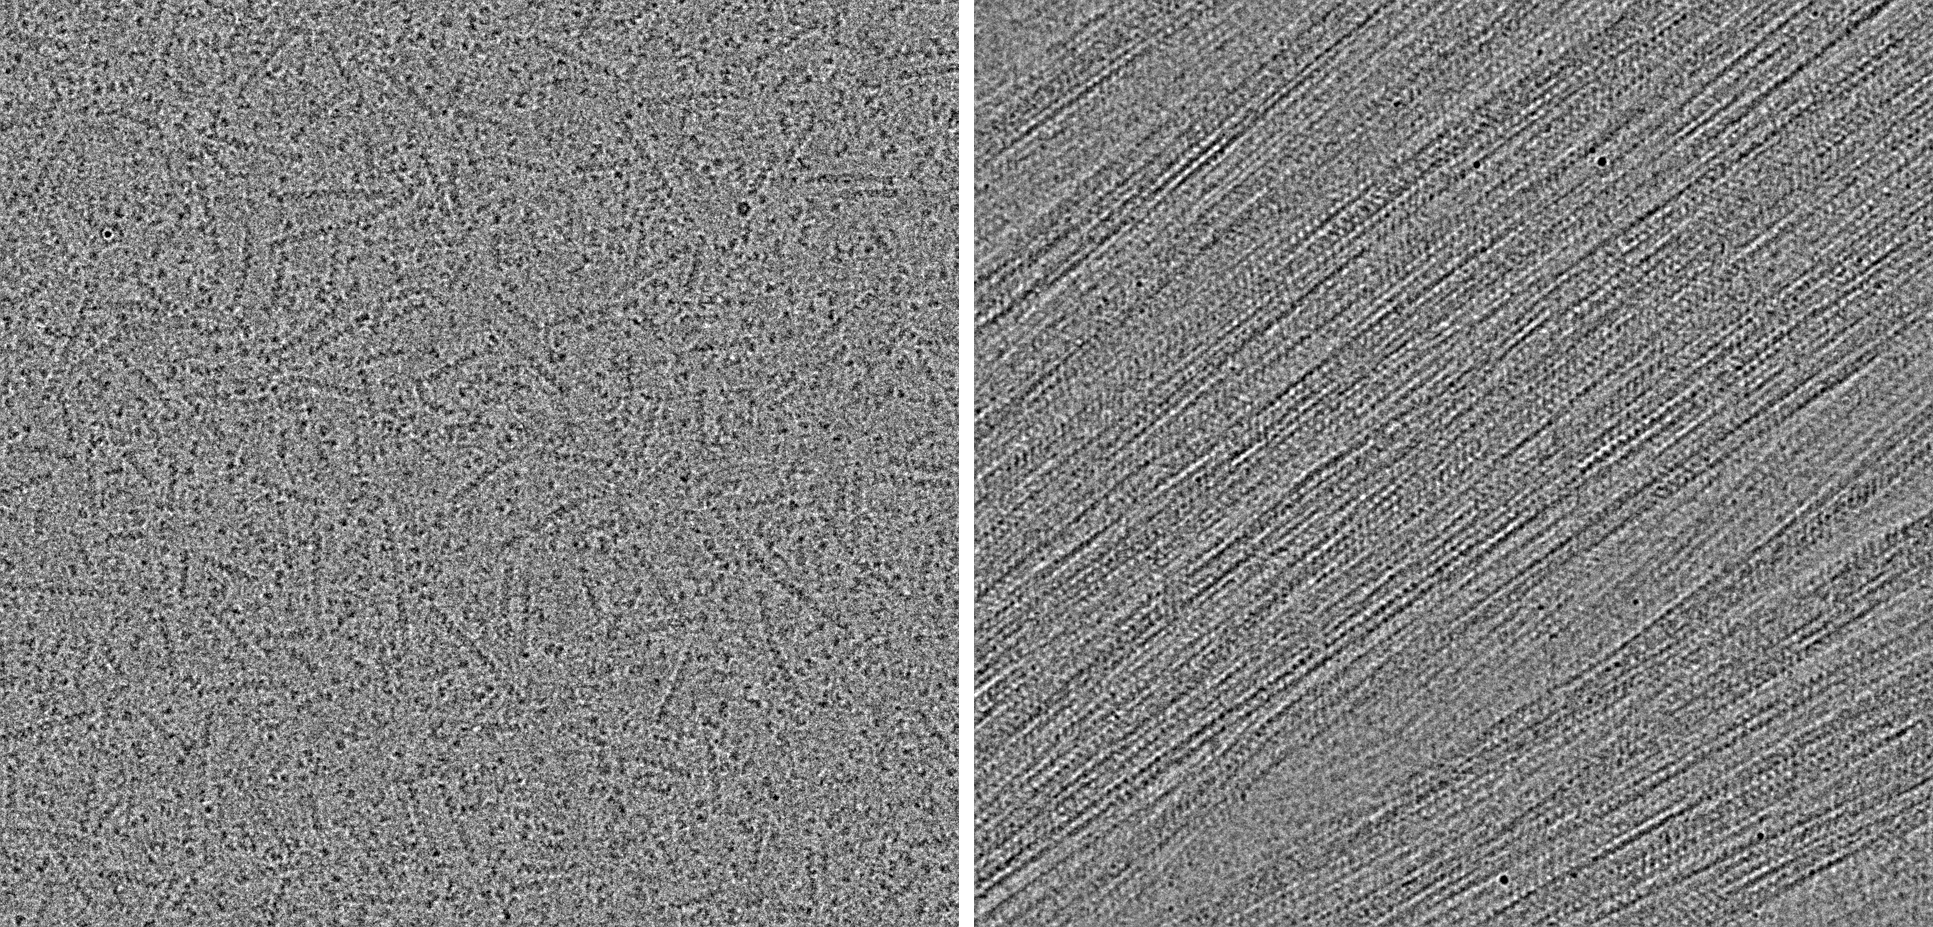
\includegraphics[width=\textwidth]{other/ftsz_mics.png}
    \titledcaption[Micrographs of FtsZ filaments]{Micrographs containing FtsZ filaments. When filaments are individual and well separated (left) they are ideal for picking and refinement. In some cases, FtsZ filaments form bundles (right) which are harder to pick, refine and classify due to the overlapping particles.}
    \label{fig:ftsz_micrographs}
\end{figure}

% TODO: data collection...?
We used CryoSPARC~\cite{punjaniCryoSPARCAlgorithmsRapid2017} for filament picking, which gave us a large amount of particles (>4M) to classify and clean up from spurious picks.
After cleaning, we ended up with about 2M particles, and very uniform classes with little variation (\autoref{fig:ftsz_classes}).
This is a typical symptom of strong preferential orientation due to the air-water interface (\fullref{em_pref_ori}), leading to a very limited range of views in the particle projections.
Although we saw hints of different views in the bundled filaments, they proved impossible to disentangle enough to obtain well-resolved classes.

\begin{figure}[ht]
    \centering
    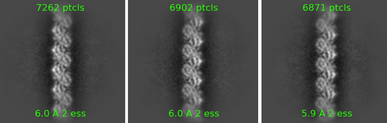
\includegraphics[width=\textwidth]{other/ftsz_classes_untilted.png}
    \titledcaption[FtsZ filament: 2D classes]{Classification results from particles with strong preferential orientation. All classes show very similar views of the FtsZ filaments, with minor variation in the out-of-plane angle.}
    \label{fig:ftsz_classes}
\end{figure}

Given the strong preferential orientation, it's unsurprising that 3D reconstructions from these particles showed very strong resolution anisotropy (while reporting \sim4 Å global resolution), so much so that we couldn't convincingly fit the monomeric model in the map (\autoref{fig:ftsz_map_bad}).

\begin{figure}[ht]
    \centering
    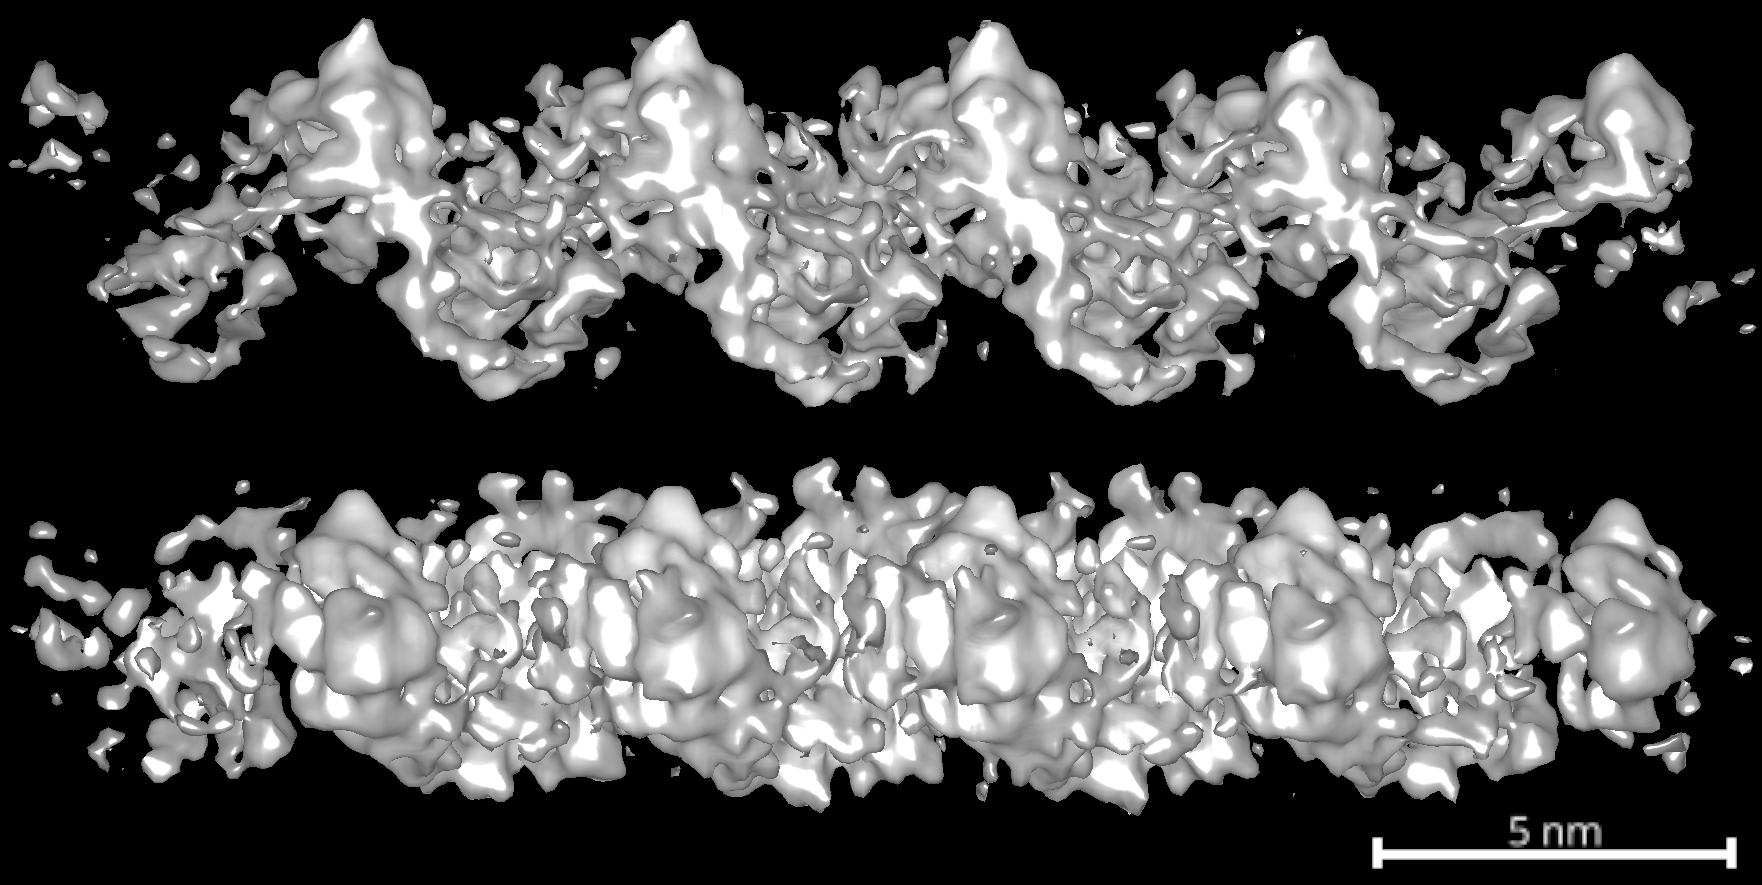
\includegraphics[width=\textwidth]{other/ftsz_map_bad.png}
    \titledcaption[FtsZ filament: anisotropic map]{FtsZ filament map affected by preferential orientation, viewed from the same direction as most 2D classes (top) and rotated by 90° (bottom) to highlight the streaking artifacts due to anisotropic orientation sampling.}
    \label{fig:ftsz_map_bad}
    % TODO: add pref orientation proof (orientation map or so)
\end{figure}

The best map currently available of FtsZ filaments (from \textit{Klebsiella pneumoniae}) also suffered from similar issues, despite the high reported resolution (\sim3 Å)~\cite{fujitaStructuresFtsZSingle2023}.

We attempted to address the issue of preferential orientation in two different ways: collecting a tilted dataset of the same samples, and preparing a new sample with methods that combat air-water interface effects.

\subsection{Graphene and streptavidin-coated grids}

We attempted to address the preferential orientation problem by using functionalized graphene grids~\cite{luFunctionalizedGrapheneGrids2022}, and streptavidin-coated affinity support grids~\cite{crucifixImmobilizationBiotinylatedDNA2004,hanLongShelflifeStreptavidin2016}.
While these approaches have been shown to work, we struggled to obtain usable grids; in the meantime, the sample prepared with the addition of detergent showed promising results, so we moved forward with it instead.

\subsection{Tilted data collection}\label{ftsz_tilted}

We prepared the sample in the same way, but this time the data collection was done with the grid at a 35° tilt.
Following the same workflow as with the untilted dataset, we then picked, classified and selected particles, obtaining a new set of class averages (\autoref{fig:ftsz_classes_tilted}).
These classes where immediately more promising than the ones from the untilted datasets, showing multiple views from the first round of classification, even in isolated filaments. % TODO: explain why these classes where better, did we get more, explain figure, what we were looking for, etc

\begin{figure}[ht]
    \centering
    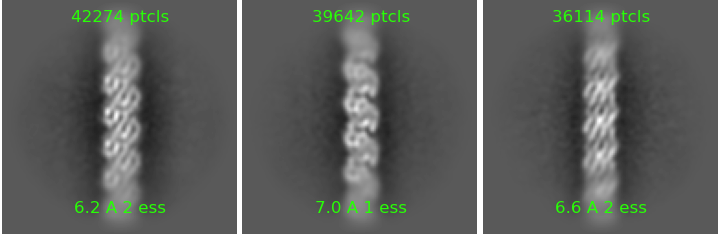
\includegraphics[width=\textwidth]{other/ftsz_classes_tilted.png}
    \titledcaption[FtsZ tilted dataset: 2D classes]{Classification results from the tilted dataset. Differently from the untilted classes, particles successfully classified into distinct views of the filament.}
    \label{fig:ftsz_classes_tilted}
\end{figure}

Despite the better view distribution of 2D classes, our 3D reconstructions had the same anisotropy issues as the untilted data.
Assuming a unform distribution of in-plane angles of the filaments (which we observed in the original dataset), a single, relatively high-tilt dataset should cover a higher portion of 3D fourier space during backprojection and thus significantly improve map isotropy~\cite{tanAddressingPreferredSpecimen2017}.

With preferentially oriented filaments collected at a fixed tilt angle, there should be a strong correlation between in-plane angle (easily identifiable from the micrograph) and the projection view (which is identified by classification). % TODO: show with synthetic dataset? Also, could it be that multiple euler combinations are redundant and correlation was just bad? How did I do this thing again?
Upon closer inspection of the picking data, however, we observed that the out-of-plane angles assigned to each particle showed no correlation with the assigned 2D class (\autoref{fig:ftsz_class_angles}).

\begin{figure}[ht]
    \centering
    \includegraphics[width=\textwidth]{example-image.png}
    \titledcaption[Out-of-plane angle by class in FtsZ titled dataset]{Out-of-plane angle plotted against the assigned 2D class. TODO}
    \label{fig:ftsz_class_angles}
\end{figure}

We soon realized that the 3D reconstruction routines of both Relion~\cite{scheresRELIONImplementationBayesian2012} and CryoSPARC~\cite{punjaniCryoSPARCAlgorithmsRapid2017} were struggling with assigning Euler angles, resulting in practically random orientations.
To impose more constraints on the refinement based on this prior knowledge on the geometry of the system, we calculated the theoretical orientation of each particle based on the in-plane angle (and assuming perfect preferential orientation), which we then used to initialize the particle poses (\fullref{stemia_angles}).

Unfortunately, this approach did not yet bear fruits: CryoSPARC does not provide fine control over angle priors and search patterns, and Relion's parameters for angle refinement proved tricky to control and resulted in orientations being either stuck in local minima, or fully randomized again (\autoref{fig:ftsz_angle_dist}).

\begin{figure}[ht]
    \centering
    \includegraphics[width=\textwidth]{example-image.png}
    \titledcaption[Angle distribution after 3D reconstruction in FtsZ tilted dataset]{TODO: angle distribution plot}
    \label{fig:ftsz_angle_dist}
\end{figure}



\subsection{Addition of detergent}

Detergent has long been used as a way to address preferential orientation and aggregation of proteins in the sample.
In our case, while it did not affect the orientation problem, it allowed FtsZ to polymerize into longer filaments without creating large bundles (\autoref{fig:ftsz_ddm_mics}).

\begin{figure}[ht]
    \centering
    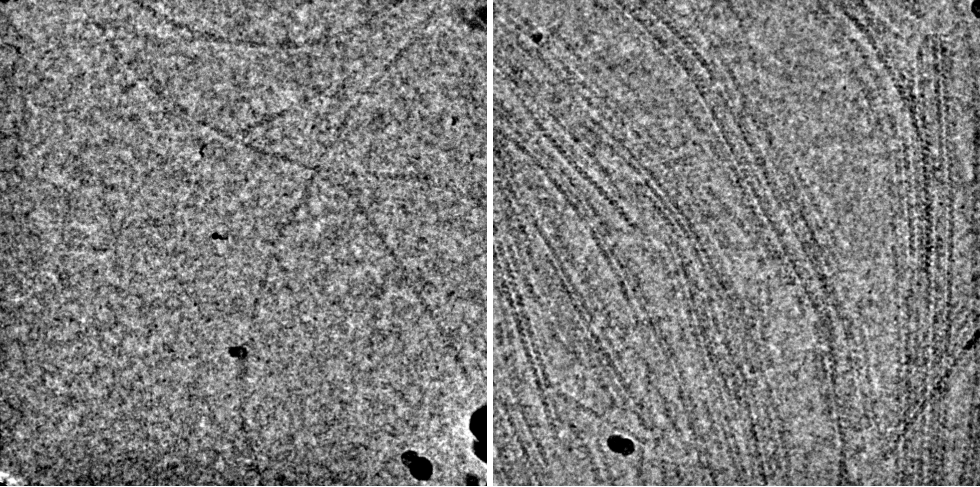
\includegraphics[width=\textwidth]{other/ftsz_mics_ddm.png}
    \titledcaption[Micrographs of FtsZ with detergent]{The addition of detergent allowed the FtsZ filaments to elongate further, without resulting in dense bundles (left). When bundles formed (right), they were often less densely packed than without detergent, opening up the possibility to pick bundled filaments in order to investigate side interactions.}
    \label{fig:ftsz_ddm_mics}
\end{figure}

The longer filaments and the very small helical twist (estimated at <1° with the previous samples), should result in different side views of the monomers being visible in the dataset.
Indeed, we observe a higher diversity in classification results, including classes with different views of single filaments (\autoref{fig:ftsz_ddm_classes_single}) and classes with two or three filaments interacting side-by-side (\autoref{fig:ftsz_ddm_classes_double}).

\begin{figure}[ht]
    \centering
    \begin{subfigure}[B]{.5\textwidth}
        \centering
        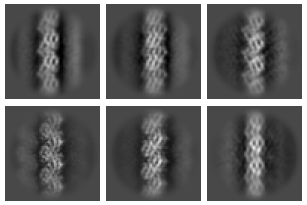
\includegraphics[width=\textwidth]{other/ftsz_classes_single.png}
        \caption{Classes with different views on single FtsZ filaments.}
        \label{fig:ftsz_ddm_classes_single}
    \end{subfigure}%
    \hfill
    \begin{subfigure}[B]{.5\textwidth}
        \centering
        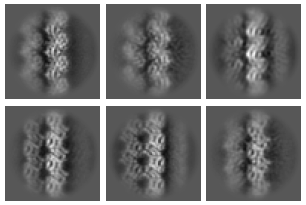
\includegraphics[width=\textwidth]{other/ftsz_classes_double.png}
        \caption{Classes with multiple interacting FtsZ filaments.}
        \label{fig:ftsz_ddm_classes_double}
    \end{subfigure}%
    \titledcaption[2D classes of FtsZ with detergent]{TODO: ftsz ddm classes}
    \label{fig:ftsz_ddm_classes}
\end{figure}

Preliminary data showed an improvement in the map interpretability, although the anisotropy due to preferential orientation is still present (\autoref{fig:ftsz_ddm_map}).

\begin{figure}[ht]
    \centering
    \includegraphics[width=\textwidth]{example-image.png}
    \titledcaption[3D map of FtsZ with detergent]{The presence of detergent helped with capturing different views of the filament, improving the orientation distribution.}
    \label{fig:ftsz_ddm_map}
\end{figure}

This project has now been taken over by Harald Bernhard, a postdoc in the MICA group, who already managed to further improve the map in a few ways.
With careful use of 2D and 3D classifications, it's possible to better isolate single filaments, which improves the initial model generation.
Balancing the different views by number of particles also improves the orientation distribution, reducing map artifacts at the cost of some global resolution.
Additionally, the use of a bigger box size in particle extraction has improved slightly the quality of the alignements and 2D class averages.
While the anisotropy issue remains, the new maps are much more interpretable, and match those by \citet{fujitaStructuresFtsZSingle2023} from \textit{K. pneumoniae} FtsZ (\autoref{fig:ftsz_hari_map}).

\begin{figure}[ht]
    \centering
    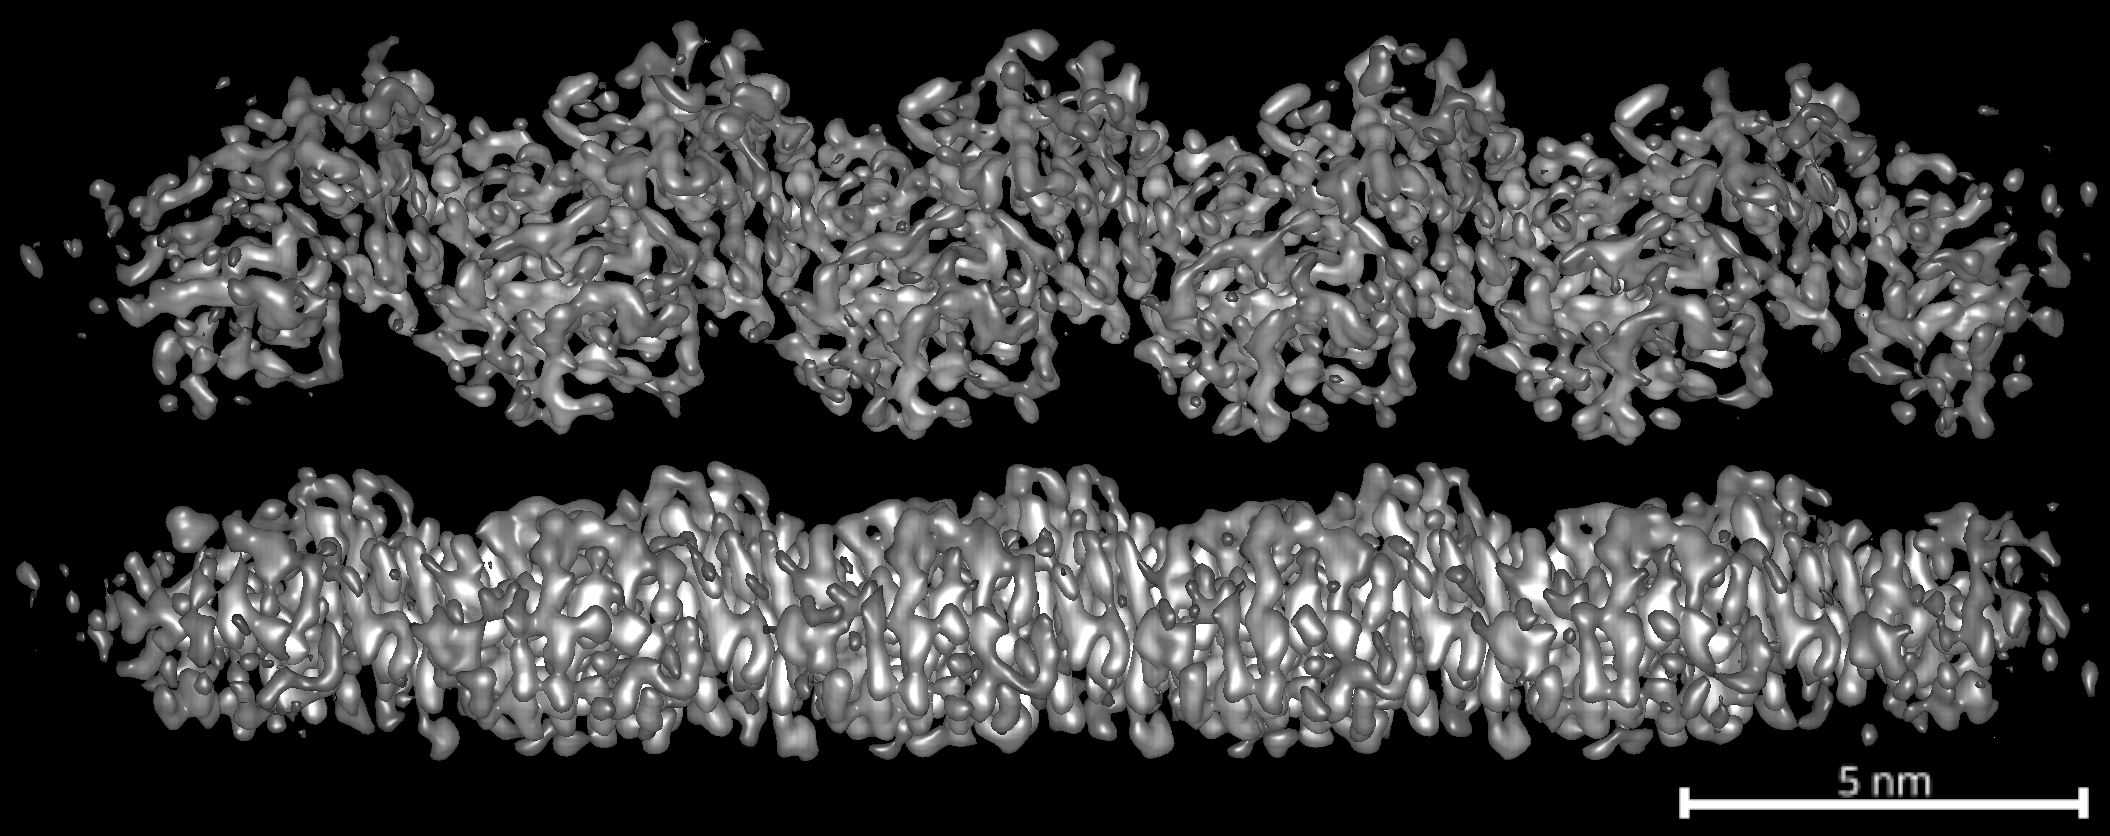
\includegraphics[width=\textwidth]{other/ftsz_map_good.png}
    \titledcaption[Our best DrFtsZ map so far]{Using the FtsZ+DDM dataset, and more careful 2D and 3D classifications to clean the dataset and better balance different views, Harald significantly improved on the FtsZ filament map. Preferential orientation is unfortunately still not fully solved, as evidenced by the streaking artifacts along one direction (bottom view), which are not present in the other (top view).}
    \label{fig:ftsz_hari_map}
\end{figure}

\section{Tomography and STA}

In parallel to the study of \textit{in vitro} FtsZ filament by SPA, we also investigated the FtsZ \textit{in situ} in the tomograms of \textit{D. radiodurans} lamellae.
Some of our findings and speculations about the 3D morphology of FtsZ are included in the \textit{D. radiodurans} manuscript (\fullref{drad_ftsz} and \fullref{ftsz_discussion}).

Our observations on the reconstructed tomograms matched those by \citet{sextonSuperresolutionConfocalCryoCLEM2022}, who also used tomography to look into D.rad and identified FtsZ and FtsA forming filaments just below the inner membrane of the septal tips (\autoref{fig:ftsz_tomo_slice}). % TODO: show more examples of this, how many have it, etc...

\begin{figure}[ht]
    \centering
    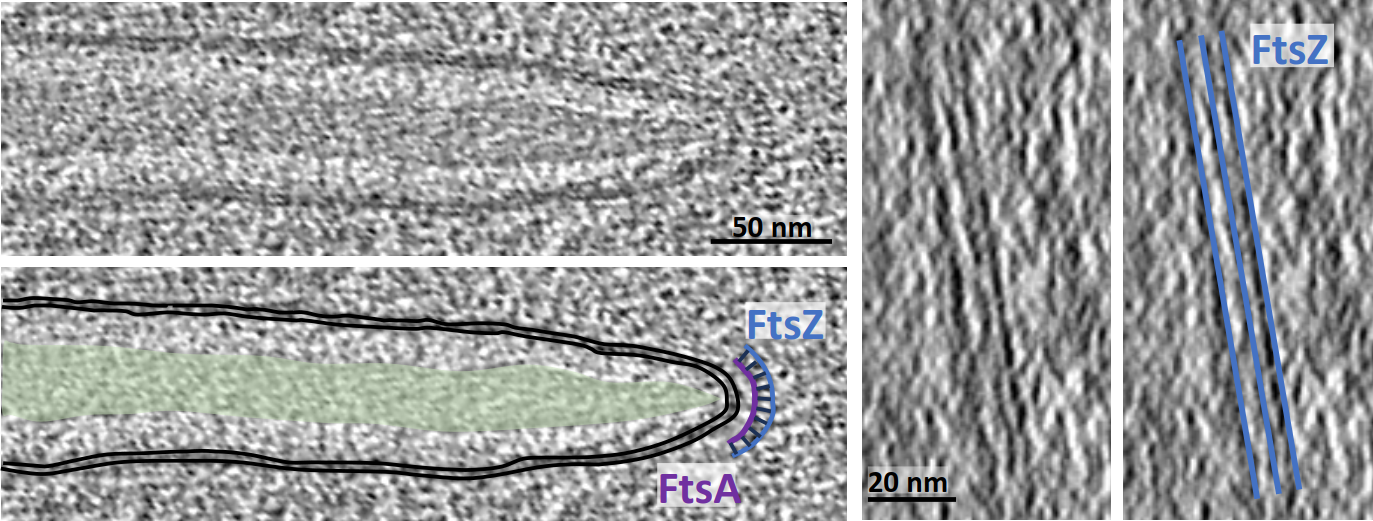
\includegraphics[width=\textwidth]{other/ftsz_slices.png}
    \titledcaption[FtsZ: tomogram slices from top and side view]{When viewing a cross-section of the bundle at the tip of the septa of \textit{D. radiodurans} (left), FtsZ is visible as a double arch separated by a gridded pattern. This is likely the result of a layer of FtsA bridging between the membrane and a layer of FtsZ filaments. (figure adapted from \autoref{drad_fig4}).}
    \label{fig:ftsz_tomo_slice}
\end{figure}

The size and spacing between FtsZ filaments is generally consistent with crystal structures and SPA studies on FtsZ filaments~\cite{mcquillenInsightsStructureFunction2020}.
the distance between FtsZ+FtsA filaments and the membrane in our tomograms is consistent with the expected \sim13-16~\cite{mcquillenInsightsStructureFunction2020}.
However, the width of the bundle appears to be smaller than the previously found 80-100 nm~\cite{mcquillenInsightsStructureFunction2020}, typically no wider than around 50-60 nm; this might be caused by differences in the thickess of the septa or modes of septation between different bacteria.

\subsection{Subtomogram averaging}

While it is clear that FtsZ and FtsA are forming filaments and bundles in vitro, and that they localize to the Z-ring in a bundle-like fashion, the details of this superstructural assembly are unknown.
To get a higher resolution view of this complex \textit{in situ}, we performed STA on particles picked from the FtsZ arches at the tips of the septa (\autoref{fig:ftsz_tomo_slice}).

Given the apparent regularity of the bundles (whose morphology appears unchanged across their length), we used blik's surface picking tool~\cite{gaifasBlikExtensible3D2024,gaifasBlikPythonTool2024}, which allows us to distribute regularly spaced particles on the sheet-like FtsZ bundles.
The inter-particle distance was chosen based on the smallest distance in the regular comb-like dark/light pattern along the FtsZ arches. % TODO: how many particles?
Two different sets of particles were thus generated: with inter-particle distance matching the visible pattern (\sim50 Å), and twice oversampled (\sim25 Å) (\autoref{fig:ftsz_tomo_picks}).

\begin{figure}[ht]
    \centering
    \begin{subfigure}[B]{.49\textwidth}
        \centering
        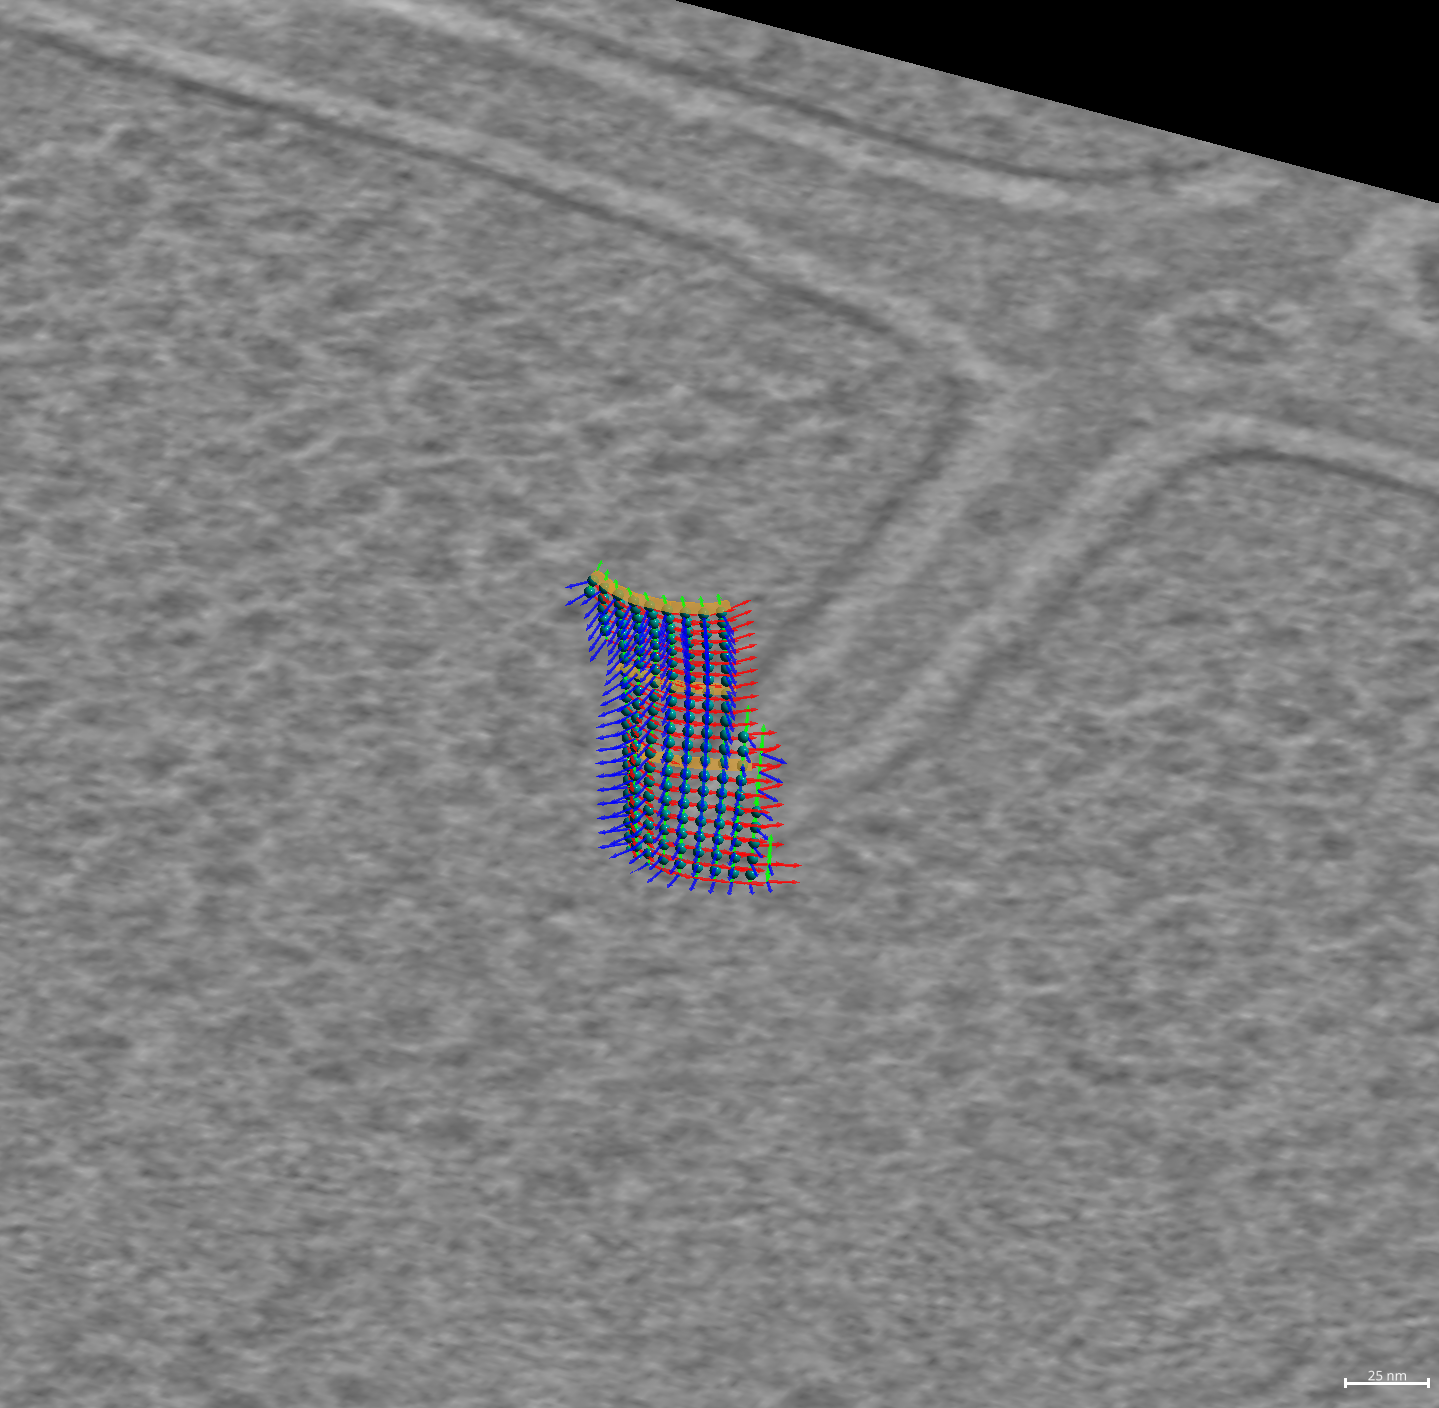
\includegraphics[width=\textwidth]{other/ftsz_particles_50A.png}
        \caption{Particle picks at 50 Å spacing.}
        \label{fig:ftsz_tomo_picks_50}
    \end{subfigure}%
    \hfill
    \begin{subfigure}[B]{.49\textwidth}
        \centering
        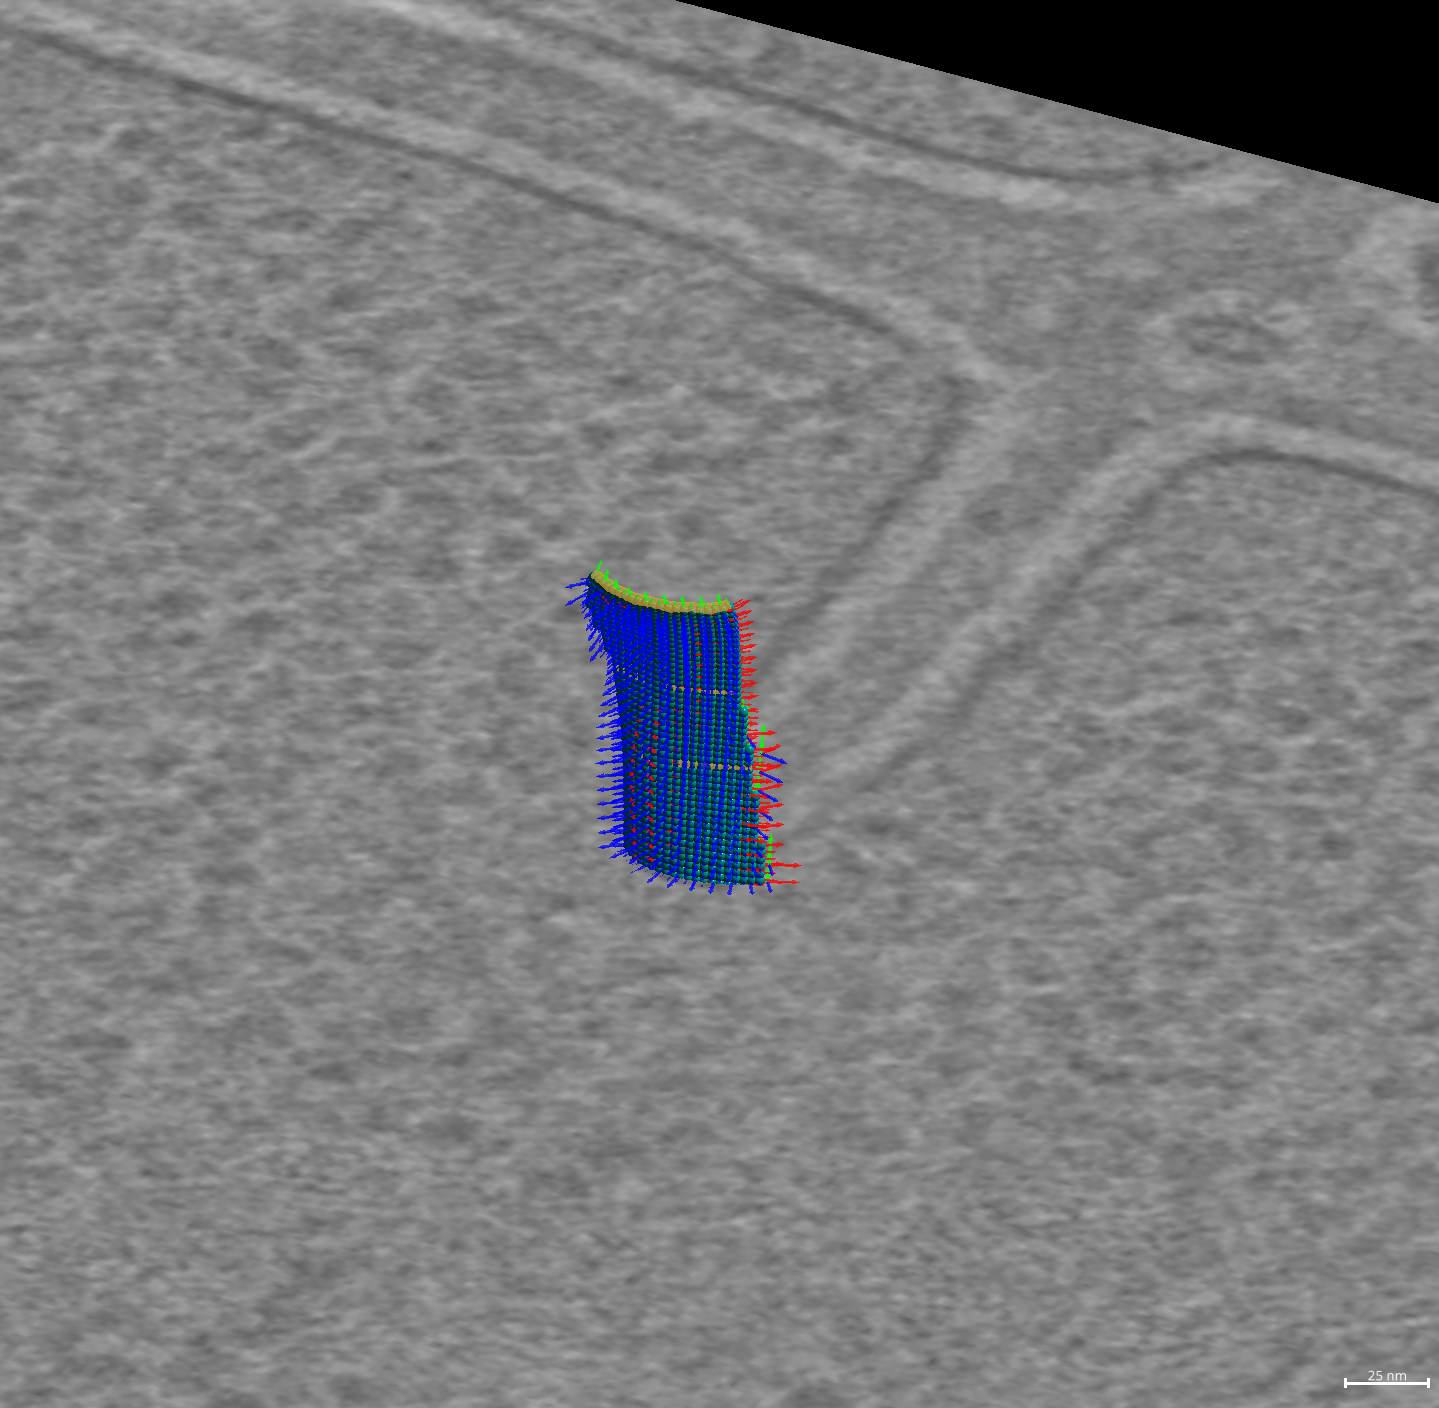
\includegraphics[width=\textwidth]{other/ftsz_particles_25A.png}
        \caption{Particle picks at 25 Å spacing.}
        \label{fig:ftsz_tomo_picks_25}
    \end{subfigure}%
    \titledcaption[Surface-based FtsZ particle picks for STA]{Particle picks on FtsZ at the tip of the septa in \textit{D. radiodurans} tomograms, generated with surface-based picking in blik~\cite{gaifasNaparipropertiesplotter2021,gaifasBlikPythonTool2024} at two different inter-particle spacings.}
    \label{fig:ftsz_tomo_picks}
\end{figure}

Subtomograms were reconstructed in Warp~\cite{tegunovRealtimeCryoelectronMicroscopy2019} using these particle picks, at different resolutions and with varying box sizes.
Using Relion~\cite{scheresRELIONImplementationBayesian2012,zivanovBayesianApproachSingleparticle2022,burtImageProcessingPipeline2024}, we performed subtomogram averaging and 3D classification to refine the positions and obtain a 3D map of the particles.
Due to the low magnification of the dataset (Nyquist \simeq9 Å), Relion was in most cases struggling to assign orientations.
The only refinement that resulted in consistent orientations and a reasonable map was with particles picked at 50 Å spacing, and subtomograms reconstructed at the highest resolution (4.346 Å/px) and with a large box size of 64 pixels, corresponding to \sim28 nm (\autoref{fig:ftsz_subtomo}).

\begin{figure}[ht]
    \centering
    \begin{subfigure}[B]{.49\textwidth}
        \centering
        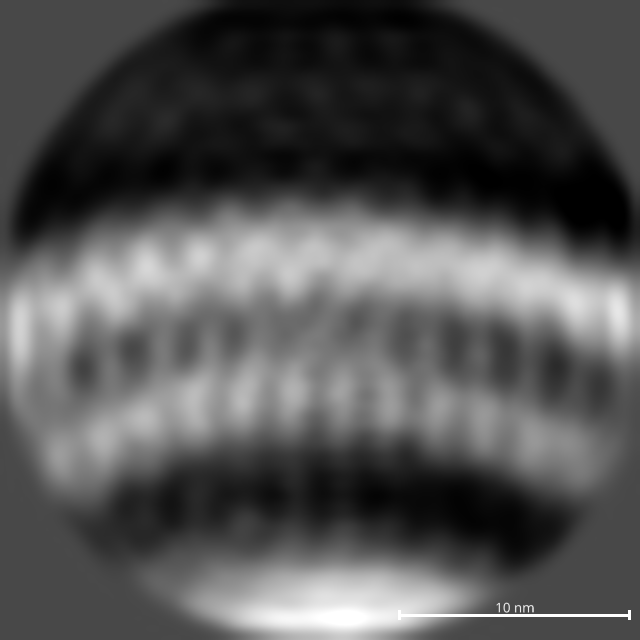
\includegraphics[width=\textwidth]{other/ftsz_subtomo_slice.png}
        \caption{Z-slice through the best FtsZ subtomogram.}
        \label{fig:ftsz_subtomo_slice}
    \end{subfigure}%
    \hfill
    \begin{subfigure}[B]{.49\textwidth}
        \centering
        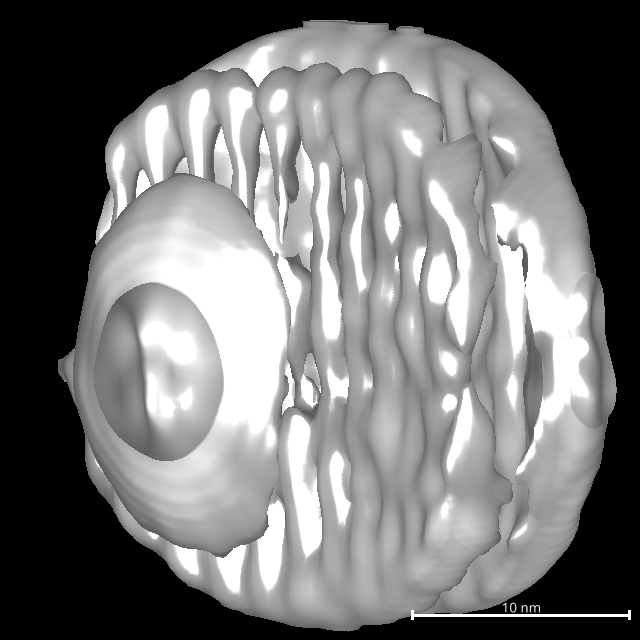
\includegraphics[width=\textwidth]{other/ftsz_subtomo_iso.png}
        \caption{Isosurface of the best FtsZ subtomogram.}
        \label{fig:ftsz_subtomo_iso}
    \end{subfigure}%
    \titledcaption[FtsZ STA preliminary results]{Subtomogram averaging results of the particle picks on FtsZ at the tip of the septa in \textit{D. radiodurans}. The grid-like pattern visible in the tomogram slices is captured by the subtomograms, but the resolution is too low for further interpretation.}
    \label{fig:ftsz_subtomo}
\end{figure}

It's worth noting that due to the nature of the division cycle of \textit{D. radiodurans}, the bacterium is generally found as a tetrad laying flat on the grid, which leads to a preferential orientation of the septa (and therefore the FtsZ filaments) along the Z axis on the tomograms.
Due to the missing wedge (\fullref{et_tomo_reconstruction}), along which the filaments are aligned, the information is blurred along the FtsZ filament axis, limiting for example the ability to distinguish individual FtsZ monomers.

\section{Discussion and future perspectives}

TODO

Ice thickness should be negligible if we do proper CTF and motion correction (iteratively)~\cite{aiyerOvercomingResolutionAttenuation2024}.

We encountered a major obstacle in the preferential orientation of filaments both in SPA and STA; the project is still ongoing and the new detergent data is currently being processed.

\section{Materials and Methods}\label{ftsz_methods}

\subsection{Sample preparation for SPA}

\subsubsection{FtsZ only}
5μl FtsZ at 12.5 mg/ml were diluted in 4 μl buffer (50 mM Tris-HCl pH 8.0, 200 mM NaCl), and 1 μl GpCpp at 10 mM.
Mix was then incubated at 25°C for 75 min to allow for filament elongation.
4μl of mix was then diluted in 16 μl of buffer (50 mM Tris-HCl pH 8.0, 200 mM NaCl), and 1 μl GpCpp at 10 mM.
The sample was then immediately frozen on R2/1 300mesh EM grids (blot time: 3.5 s).

\subsubsection{FtsZ+DDM}
2μl FtsZ at 12.5 mg/ml were diluted in 16 μl buffer (50 mM Tris-HCl pH 8.0, 200 mM NaCl), and 2 μl GpCpp at 10 mM.
Mix was then incubated at 25°C for 30 min to allow for filament elongation, after which 2μl DDM at 0.09\% was added.
Grids were frozen with and without further 5x dilution in buffer (50 mM Tris-HCl pH 8.0, 200 mM NaCl, 1 mM GpCpp, 0.009\% DDM: 2 μl mix + 8 μl buffer)

TODO: should we include details about reproducibility/elongation? I added some to the text above, but maybe we need more details here.

TODO: graphene and streptavidin grids

\subsection{Data Collection for SPA}

TODO: I need help here for the technical microscopy details...

\subsection{SPA processing}

filament picking (parameters, issues with length)

link to \fullref{stemia_angles}.

\subsection{\textit{D. radiodurans} lamellae and tomography data collection}

See \fullref{drad_lamellae_method} and \fullref{drad_tomo_method}.

\subsection{STA data processing}

blik, relion

        \chapter{Side projects}

\begin{outline}
\1 projection matching for eymi's work
\1 cs2star
\1 
\end{outline}

    \part{Discussion}
        \chapter{Conclusions, Discussion and Future Perspectives}

The hardest part...

\localtableofcontents

\begin{outline}
\1 usefulness of blik in working with data and developing new tools
    \2 especially good here to mention other projects that benefited from this work (either blik or related tools)
\1 new insights into D.rad
\1 evolution of field during thesis, new software, new people... new initiatives (some words on teamtomo maybe should go here as well!)
\1 scipion (need to finish that...)
\1 I'd like to have a general section about software practices, but not sure where
    \2 a case for user-friendliness (cryosparc > relion)
    \2 a case for open-source (relion > cryosparc)
    \2 a case for domain agnosticism (napari)
    \2 the benefits of modularity, "clean code", documentation, etc, to the research community
\end{outline}


\backmatter
    \bookmarksetup{startatroot}  % end \part in the bookmarks
    \listoffigures
    \listoftables
    \chapter{Glossary}

\renewcommand{\arraystretch}{1.5}

\begin{tabularx}{\linewidth}{>{\bf}l X}
Cryo-EM & Cryo-electron microscopy \\
Cryo-ET & Cryo-electron tomography \\
CTF & Contrast Transfer Function \\
PS & Power Spectrum \\
CC & Cross-correlation \\
SPA & Single particle analysis \\
STA & Subtomogram averaging \\
ND & N-dimensional \\
\end{tabularx}

% TODO: sort alphabetically

    \bibliography{./bibliography.bib}

\end{document}

% TODO: make sure chapter have short names for the header and TOCs in []
% TODO: same thing as above but for figures
% TODO: add CV at the end?
% TODO: should introduction be a brief thing at the beginning, or include everything up to the bil_paper?
% TODO: use tikz for diagram describing blik stuff (surfaces and such)
% TODO: take care of all the overfull/underfull nonsense
% TODO: add quotes for chapters/sections
% TODO: check spelling and maybe run a grammar/syntax checker too.
% TODO: add code to generate figures when possible
